\documentclass[11pt]{article}
\usepackage{iftex}
\ifPDFTeX
  \usepackage[T1]{fontenc}
  \usepackage[utf8]{inputenc}
\else
  \usepackage{unicode-math}
  \defaultfontfeatures{Scale=MatchLowercase}
  \defaultfontfeatures[\rmfamily]{Ligatures=TeX,Scale=1}
\fi
\usepackage{lmodern}
\usepackage[margin=0.88in,headheight=16pt,headsep=14pt,footskip=28pt]{geometry}
\usepackage{microtype}
\usepackage[dvipsnames,svgnames,x11names]{xcolor}
\usepackage{amsmath,mathtools}
\usepackage{graphicx}
\usepackage{booktabs,longtable,array,calc,tabularx}
\usepackage{float}
\usepackage{caption}
\usepackage[most]{tcolorbox}
\usepackage{titlesec}
\usepackage{fancyhdr}
\usepackage{enumitem}
\usepackage{etoolbox}
\usepackage{hyperref}
\usepackage{bookmark}
\usepackage{xurl}
\usepackage{ragged2e}
\usepackage{listings}
\usepackage{newunicodechar}
\newunicodechar{α}{\ensuremath{\alpha}}
\newunicodechar{𝛼}{\ensuremath{\alpha}}

\definecolor{AgiBlue}{HTML}{153B6A}
\definecolor{AgiGold}{HTML}{8A6A1F}
\definecolor{AgiSlate}{HTML}{334155}
\definecolor{AgiMist}{HTML}{F7F7F4}
\definecolor{AgiInk}{HTML}{111827}
\definecolor{AgiLine}{HTML}{D7DEE8}

\hypersetup{colorlinks=true,linkcolor=AgiBlue,citecolor=AgiBlue,urlcolor=AgiBlue,pdfauthor={Vincent Boucher},pdftitle={AGI ALPHA as a Far-From-Equilibrium Multi-Agent Work Engine}}
\urlstyle{same}
\graphicspath{{./}}
\setkeys{Gin}{keepaspectratio}
\captionsetup{font=small,labelfont={bf,color=AgiBlue},labelsep=period,skip=7pt}
\setcounter{secnumdepth}{0}
\setlength{\parindent}{0pt}
\setlength{\parskip}{0.58em plus 0.12em minus 0.06em}
\linespread{1.035}
\RaggedRight
\emergencystretch=9em
\Urlmuskip=0mu plus 3mu
\setlist[itemize]{leftmargin=1.5em,itemsep=0.15em,topsep=0.25em,parsep=0pt}
\setlist[enumerate]{leftmargin=1.7em,itemsep=0.18em,topsep=0.25em,parsep=0pt}
\renewcommand{\arraystretch}{1.15}
\setlength{\tabcolsep}{5pt}
\setlength{\LTpre}{0.45em}
\setlength{\LTpost}{0.45em}
\AtBeginEnvironment{longtable}{\small\RaggedRight
\emergencystretch=9em
\Urlmuskip=0mu plus 3mu}
\AtBeginEnvironment{figure}{\centering}
\providecommand{\tightlist}{\setlength{\itemsep}{0pt}\setlength{\parskip}{0pt}}

\titleformat{\section}{\Large\bfseries\color{AgiBlue}}{}{0em}{}[\vspace{-0.15em}{\color{AgiLine}\titlerule}]
\titleformat{\subsection}{\large\bfseries\color{AgiSlate}}{}{0em}{}
\titleformat{\subsubsection}{\normalsize\bfseries\color{AgiSlate}}{}{0em}{}
\titlespacing*{\section}{0pt}{1.35em}{0.55em}
\titlespacing*{\subsection}{0pt}{1.05em}{0.35em}
\titlespacing*{\subsubsection}{0pt}{0.85em}{0.25em}

\pagestyle{fancy}
\fancyhf{}
\fancyhead[L]{\small\textsc{AGI ALPHA}}
\fancyhead[R]{\small\textsc{$\alpha$-AGI Ascension}}
\fancyfoot[C]{\small\thepage}
\renewcommand{\headrulewidth}{0.25pt}
\renewcommand{\footrulewidth}{0pt}

\newtcolorbox{executivebox}{enhanced,breakable,colback=white,colframe=AgiBlue!42,boxrule=0.6pt,arc=3pt,left=9pt,right=9pt,top=8pt,bottom=8pt}
\newtcolorbox{goldbox}{enhanced,breakable,colback=AgiBlue!3,colframe=AgiGold!55,boxrule=0.55pt,arc=3pt,left=8pt,right=8pt,top=7pt,bottom=7pt}

\lstset{
  basicstyle=\ttfamily\scriptsize,
  breaklines=true,
  breakatwhitespace=true,
  columns=fullflexible,
  frame=single,
  rulecolor=\color{AgiLine},
  backgroundcolor=\color{AgiMist},
  xleftmargin=0.5em,
  xrightmargin=0.5em,
  aboveskip=0.6em,
  belowskip=0.6em
}

\newtcolorbox{titlebox}{enhanced,colback=white,colframe=AgiBlue!45,boxrule=0.6pt,arc=4pt,left=12pt,right=12pt,top=12pt,bottom=12pt}

\usepackage{fancyvrb}
\newcommand{\VerbBar}{|}
\newcommand{\VERB}{\Verb[commandchars=\\\{\}]}
\DefineVerbatimEnvironment{Highlighting}{Verbatim}{commandchars=\\\{\}}
% Add ',fontsize=\small' for more characters per line
\newenvironment{Shaded}{}{}
\newcommand{\AlertTok}[1]{\textcolor[rgb]{1.00,0.00,0.00}{\textbf{#1}}}
\newcommand{\AnnotationTok}[1]{\textcolor[rgb]{0.38,0.63,0.69}{\textbf{\textit{#1}}}}
\newcommand{\AttributeTok}[1]{\textcolor[rgb]{0.49,0.56,0.16}{#1}}
\newcommand{\BaseNTok}[1]{\textcolor[rgb]{0.25,0.63,0.44}{#1}}
\newcommand{\BuiltInTok}[1]{\textcolor[rgb]{0.00,0.50,0.00}{#1}}
\newcommand{\CharTok}[1]{\textcolor[rgb]{0.25,0.44,0.63}{#1}}
\newcommand{\CommentTok}[1]{\textcolor[rgb]{0.38,0.63,0.69}{\textit{#1}}}
\newcommand{\CommentVarTok}[1]{\textcolor[rgb]{0.38,0.63,0.69}{\textbf{\textit{#1}}}}
\newcommand{\ConstantTok}[1]{\textcolor[rgb]{0.53,0.00,0.00}{#1}}
\newcommand{\ControlFlowTok}[1]{\textcolor[rgb]{0.00,0.44,0.13}{\textbf{#1}}}
\newcommand{\DataTypeTok}[1]{\textcolor[rgb]{0.56,0.13,0.00}{#1}}
\newcommand{\DecValTok}[1]{\textcolor[rgb]{0.25,0.63,0.44}{#1}}
\newcommand{\DocumentationTok}[1]{\textcolor[rgb]{0.73,0.13,0.13}{\textit{#1}}}
\newcommand{\ErrorTok}[1]{\textcolor[rgb]{1.00,0.00,0.00}{\textbf{#1}}}
\newcommand{\ExtensionTok}[1]{#1}
\newcommand{\FloatTok}[1]{\textcolor[rgb]{0.25,0.63,0.44}{#1}}
\newcommand{\FunctionTok}[1]{\textcolor[rgb]{0.02,0.16,0.49}{#1}}
\newcommand{\ImportTok}[1]{\textcolor[rgb]{0.00,0.50,0.00}{\textbf{#1}}}
\newcommand{\InformationTok}[1]{\textcolor[rgb]{0.38,0.63,0.69}{\textbf{\textit{#1}}}}
\newcommand{\KeywordTok}[1]{\textcolor[rgb]{0.00,0.44,0.13}{\textbf{#1}}}
\newcommand{\NormalTok}[1]{#1}
\newcommand{\OperatorTok}[1]{\textcolor[rgb]{0.40,0.40,0.40}{#1}}
\newcommand{\OtherTok}[1]{\textcolor[rgb]{0.00,0.44,0.13}{#1}}
\newcommand{\PreprocessorTok}[1]{\textcolor[rgb]{0.74,0.48,0.00}{#1}}
\newcommand{\RegionMarkerTok}[1]{#1}
\newcommand{\SpecialCharTok}[1]{\textcolor[rgb]{0.25,0.44,0.63}{#1}}
\newcommand{\SpecialStringTok}[1]{\textcolor[rgb]{0.73,0.40,0.53}{#1}}
\newcommand{\StringTok}[1]{\textcolor[rgb]{0.25,0.44,0.63}{#1}}
\newcommand{\VariableTok}[1]{\textcolor[rgb]{0.10,0.09,0.49}{#1}}
\newcommand{\VerbatimStringTok}[1]{\textcolor[rgb]{0.25,0.44,0.63}{#1}}
\newcommand{\WarningTok}[1]{\textcolor[rgb]{0.38,0.63,0.69}{\textbf{\textit{#1}}}}

\begin{document}
\begin{titlepage}
\thispagestyle{empty}
\pagecolor{AgiMist}
\vspace*{0.7cm}
\begin{center}
\begin{tcolorbox}[enhanced,width=0.86\textwidth,colback=white,colframe=AgiLine,boxrule=0.55pt,arc=3pt,left=8pt,right=8pt,top=8pt,bottom=8pt]
\centering\Large\textsc{MONTREAL.AI / QUEBEC.AI}
\end{tcolorbox}
\vspace{1.05cm}
\begin{tcolorbox}[enhanced,width=0.92\textwidth,colback=white,colframe=AgiBlue!45,boxrule=0.6pt,arc=4pt,left=12pt,right=12pt,top=12pt,bottom=12pt]
\centering
{\fontsize{29}{34}\selectfont\bfseries\color{AgiBlue} AGI ALPHA as a\\[0.18em] Far-From-Equilibrium\\[0.18em] Multi-Agent Work Engine\par}
\vspace{0.45cm}
{\Large A Gibbs--Game--Hamiltonian Framework for $\alpha$-AGI Ascension\par}
\end{tcolorbox}
\vspace{0.8cm}
{\Large\bfseries Vincent Boucher\par}
\vspace{0.12cm}
{\normalsize President of MONTREAL.AI and QUEBEC.AI\par}
{\normalsize Written with AI\par}
\vspace{0.12cm}
{\normalsize April 26, 2026\par}
\vspace{0.75cm}
\begin{executivebox}
\textbf{Executive premise.} AGI ALPHA is modeled as a far-from-equilibrium agentic work engine whose organized complexity is sustained by continuous inflows of compute, data, tasks, incentives, and feedback. The framework integrates Gibbs-like free-energy objectives, statistical physics, Hamiltonians, game theory, and validator-gated coordination into a scientific theory of large-scale multi-agent systems oriented toward verified external impact, scientific discovery, energy abundance, civilizational-scale productive capacity, real-task demonstration under explicit safety gates, and experience-grounded learning from long streams of tool, validator, reward, settlement, and delayed-outcome events.
\end{executivebox}
\vfill
\begin{goldbox}
\centering\small\textbf{Keywords:} nonequilibrium organization; Gibbs free energy; statistical physics; Hamiltonians; multi-agent systems; validator-gated coordination; real-task demonstrations; mechanism design; agentic AI; experience-grounded coordination
\end{goldbox}
\end{center}
\end{titlepage}

\section{Abstract}\label{abstract}

This paper develops a scientific framework for \textbf{AGI ALPHA} and
\textbf{α-AGI Ascension} as a far-from-equilibrium, validator-gated,
multi-agent work engine. The central thesis is that large-scale agentic
coordination becomes operationally ``alive'' when continuous inflows of
compute, data, tasks, incentives, and feedback sustain organized
complexity that would otherwise decay into idle equilibrium, chaotic
search, or brittle over-centralization. The framework integrates
nonequilibrium thermodynamics, Gibbs-like free-energy objectives,
statistical physics, Hamiltonian dynamics, game-theoretic mechanism
design, multi-agent reinforcement learning, and contemporary agentic-AI
deployment practice. We distinguish literal thermodynamic energy at the
compute layer from formal free-energy analogues at the coordination
layer. We then define measurable conditions for α-AGI Ascension:
positive verified work output, bounded risk, productive swarm entropy,
reliable credit assignment, validator precision, and impact-adjusted
free-energy descent. The paper contributes a formal vocabulary, an
architecture, a substrate-level distinction between intelligence models
and intelligence organizations, a set of monitoring metrics, a real-task
demonstration standard and minimal viable reference implementation for
scalable/efficient/safe coordination, a civilizational-scale value
horizon, a doctrine synthesis of the AGI Alpha corpus, and a frontier
research synthesis across evolved coordinators, agentic organization,
self-improving software agents, distributional safety, artificial life,
scientific discovery systems, symbolic compression, self-play limits,
and production-grade tool actuation. The research program turns agentic
activity into externally verified impact without confusing maximum
impact with unconstrained autonomy, and it adds a real-task
demonstration gate: scalability, efficiency, and safety claims count
only when they are supported by benchmarked tasks, reproducible traces,
external validators, and cost/risk accounting. It further grounds
scientific discovery in generalized validated search: directed evolution
shows that real assays can substitute for omniscient prediction, while
DISCO-style multimodal generative design shows that global proposal can
supply novel evolvable starting points; AGI ALPHA generalizes this
proposal-validation-lineage-compression loop from proteins to
organizations of agents, tools, artifacts, validators, memory,
incentives, and governance. Building on the Era of Experience thesis, AGI ALPHA treats evidence bundles and grounded tool interactions as long-lived experience streams from which routers, world models, reward ledgers, and governance policies can improve. Building on value-relevant learned planning, AGI ALPHA further defines ProofZero planning: a commercially independent layer that searches over abstract evidence states to predict grounded reward, routing policy, future verified value, and validator/safety/cost outcomes before acting.

\section{Core claim}\label{core-claim}

The most rigorous compressed claim is:

\[
\boxed{
\alpha\text{-AGI Ascension}
=
\text{bounded, far-from-equilibrium, multi-agent work production}
}
\]

or, in operational form:

\[
\boxed{
\dot{E}_{\text{compute,data,capital,tasks}}
\rightarrow
\dot{W}_{\text{verified impact}}
+
\dot{Q}_{\text{dissipated search}}
+
\dot{I}_{\text{memory}}
}
\]

AGI ALPHA brings α-AGI Ascension to life when energy-mediated
computation becomes a continuously replenished, statistically mapped,
learned-and-Hamiltonian-routed, game-theoretically aligned,
validator-gated swarm that converts open-system inflows into verified,
risk-bounded work. The router is not a single hand-coded scorer; it is a
family of commercially independent coordination substrates that learn
when to decompose, delegate, verify, stop, escalate, and remember.

\section{Model substrate vs.~organizational
substrate}\label{model-substrate-vs.-organizational-substrate}

The Transformer revealed a scalable substrate for intelligence
\emph{inside models}: a general architecture in which tokens, attention,
depth, parameters, data, and compute could compound into increasingly
capable representation, prediction, and reasoning systems {[}56{]}. AGI
ALPHA proposes the analogous substrate \emph{above models}: a scalable
architecture for intelligence organizations, where agents, jobs,
validators, memory, incentives, markets, governance, and settlement
compound into increasingly capable systems of verified work.

The distinction is structural. The Transformer made intelligence
scalable as computation; AGI ALPHA aims to make intelligence scalable as
institution. In this framing, α-AGI Ascension is not merely many agents
communicating. It is the emergence of an organizational substrate in
which intelligence can be routed, validated, priced, remembered,
governed, and recursively improved.

\[
\text{Transformer}=\mathcal{S}_{\text{model}}(\text{tokens},\text{attention},\text{parameters},\text{data},\text{compute})
\]

\[
\text{AGI ALPHA}=\mathcal{S}_{\text{organization}}(\text{agents},\text{jobs},\text{validators},\text{memory},\text{incentives},\text{governance})
\]

\begin{figure}
\centering

\includegraphics[width=0.96\textwidth,height=\textheight]{figures_png/figure14_model_vs_organization_substrate.png}
\caption{Model substrate versus organizational substrate. The
Transformer scales intelligence inside models; AGI ALPHA proposes a
substrate for scaling intelligence across governed organizations of
agents, jobs, validators, memory, incentives, and governance.}
\end{figure}

\textbf{Transformer scaled intelligence in models; AGI ALPHA scales
intelligence in organizations.}

This substrate framing clarifies the paper's strategic thesis. The next
frontier is not only larger models, but governed intelligence
organizations that convert model capability into proof-bearing labor,
market activity, scientific discovery, capital formation, and
energy-scale infrastructure under auditable constraints.

\section{Scope and scientific claim
boundaries}\label{scope-and-scientific-claim-boundaries}

This manuscript is a theoretical systems paper. It does \textbf{not}
claim that unrestricted artificial general intelligence has been
achieved. It does \textbf{not} claim that autonomous economic
sovereignty, autonomous legal agency, or mainnet-scale economic proof
has been validated. It also does \textbf{not} treat internal
demonstrations as sufficient evidence of external impact. Instead, the
paper gives a formal model and a measurement program for testing whether
a large-scale multi-agent system has entered a sustained, useful,
governed, far-from-equilibrium coordination regime.

Public AGI Alpha materials frame α-AGI Architect as an operational
blueprint for scalable multi-agent deployment and strategic
infrastructure {[}16{]}. This manuscript treats that framing as a
proposed system architecture to be formalized and tested, not as
empirical proof of achieved AGI.

The phrase ``to bring to life'' is used in an engineering and cybernetic
sense. A biological organism and an AI protocol are not the same class
of object. The relevant analogy is the \textbf{dissipative structure}: a
form of order sustained only while coupled to an environment that
supplies energy, matter, information, and constraints. Prigogine's
nonequilibrium thermodynamics made this type of order central to the
study of far-from-equilibrium systems {[}1{]}. In an agentic system, the
sustained flows are compute, data, tasks, incentives, validation,
feedback, policy, and tool access.

\section{Institutional doctrine
synthesis}\label{institutional-doctrine-synthesis}

The AGI Alpha corpus supplied for this paper is treated as a strategic
primary-source doctrine, not as empirical validation of unrestricted
AGI. Its recurring architecture can be summarized as a sovereign
synthetic labor stack: identity-bound agents, validator-gated jobs,
proof-bearing work, reputation-weighted settlement, public memory,
on-chain governance, recursive improvement controls, and reinvestment
into compute, science, infrastructure, and energy capacity. Public
repositories and public mainnet contract pages provide the operational
vocabulary for this stack: AGI Jobs as market, Alpha nodes as workers,
Meta-Agentic cognition as the coordination layer, \(AGIALPHA\) as
incentive substrate, and ENS-backed job pages as durable public memory
{[}19-23{]}.

In this synthesis, \textbf{AI sovereignty} means the capacity of an
institution, nation, or protocol to command verifiable machine labor
without surrendering identity, memory, settlement, or governance to an
opaque external monopoly. \textbf{The agent-native economy} means a
market in which machines can discover work, bid, execute, prove, settle,
update reputation, and route future labor under auditable rules.
\textbf{Recursive self-improvement governance} means that improvement is
permitted only through traceable, permissioned, validator-reviewed
updates rather than unbounded self-modification.

The doctrine is therefore not merely accelerationist. It is a control
architecture: autonomy measured, work proven, value settled, memory made
public, and scale constrained by governance before it compounds into
larger industrial and energy systems.

\begin{figure}
\centering
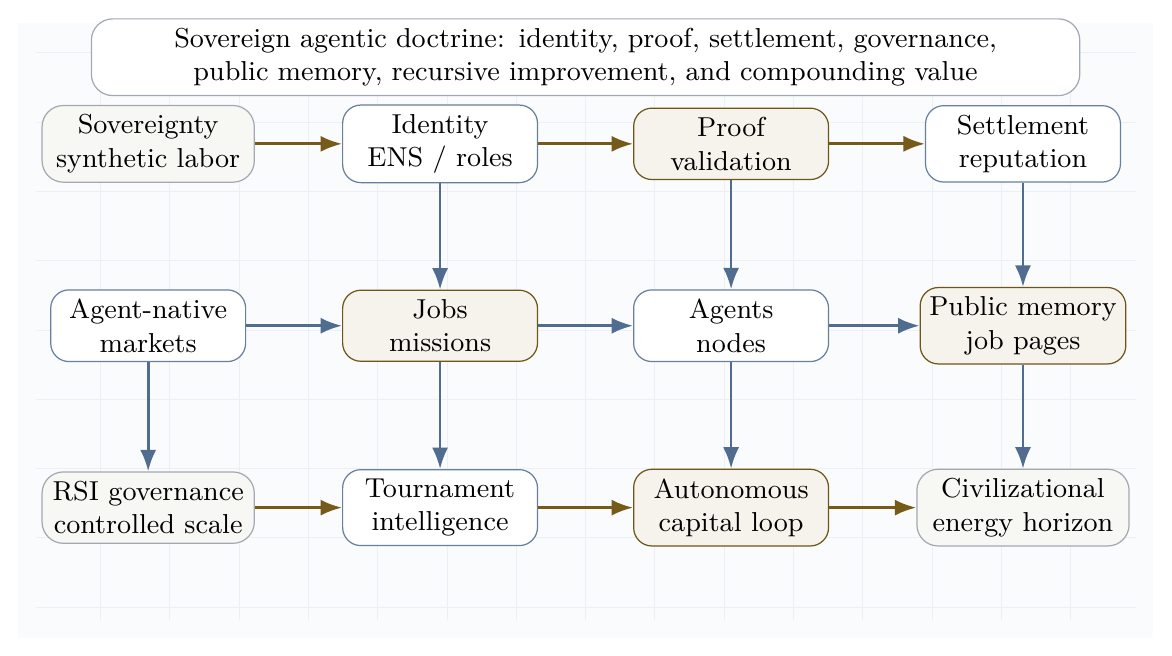
\includegraphics[width=0.96\textwidth,height=\textheight]{figures_png/figure9_doctrine_lattice.png}
\caption{Sovereign agentic doctrine lattice. The supplied AGI Alpha
corpus is synthesized into an institutional stack: identity, proof,
settlement, governance, public memory, recursive improvement, autonomous
capital, and a civilizational energy horizon.}
\end{figure}


\section{Contributions}\label{contributions}

This paper makes twenty contributions.

\begin{enumerate}
\def\labelenumi{\arabic{enumi}.}
\tightlist
\item It defines $\alpha$-AGI Ascension as a measurable nonequilibrium regime rather than an undefined emergence claim.
\item It introduces an operational Gibbs-like free-energy functional for multi-agent coordination.
\item It distinguishes the Transformer as a scalable substrate for intelligence models from AGI ALPHA as a scalable substrate for intelligence organizations.
\item It introduces a real-task demonstration harness for scalable, efficient, and safe multi-agent coordination across software engineering, policy-bound tool use, assistant research, web and desktop automation, and scientific workflows.
\item It specifies a minimal viable AGI ALPHA implementation: a validator-gated, trace-producing, benchmarkable multi-agent CI/CD and evaluation harness.
\item It upgrades the coordination layer from a single Hamiltonian router to a learned router family spanning natural-language workflow routers, evidence-state lightweight routers, evolutionary coordinators, reinforcement-learned coordinators, and hybrid task/risk/cost-aware routers.
\item It models agent constellations with statistical physics and Hamiltonian interaction terms.
\item It connects game-theoretic incentives to validator-gated mechanism design.
\item It gives a detailed theory of the continuous inflows needed to sustain organized agentic complexity.
\item It synthesizes the AGI Alpha doctrine into a sovereign agentic stack: identity, proof, settlement, governance, public memory, recursive improvement, autonomous capital, and energy-scale capacity.
\item It frames a governed Type-II / star-scale energy horizon as an asymptotic value target rather than a present-day achievement claim.
\item It proposes metrics and experiments for falsifying, improving, or validating the framework.
\item It introduces an anti-untethering constraint for self-play and self-training.
\item It frames build-test-symbolic-compression as the mechanism that converts sparse evidence into reusable design knowledge.
\item It distinguishes automation markets from sovereign invention engines.
\item It specifies a distributional safety envelope for populations of interacting agents.
\item It reframes directed evolution and DISCO-style biomolecular design as scientific inspiration for generalized validated search, while keeping AGI ALPHA commercially independent from third-party protein-design methods.
\item It defines AGI ALPHA-native method families: Validated Organizational Evolution, Proof-Gradient Routing, Assay-Equivalent Validator Lattices, Evidence-Bundle Memory, Artifact-Lineage Search, Coordination Fitness Landscapes, and the Build-Test-Compress-Evolve Control Plane.
\item It upgrades AGI ALPHA into an experience-grounded coordination substrate with Sovereign Experience Streams, Grounded Reward Ledgers, Validator-Reward Separation, world-model planning, temporal options, and experience quarantine/replay.
\item It introduces a commercially independent ProofZero Planning Layer: value-relevant learned planning over latent evidence states, validator-aware bounded tree search, Evidence Reanalyze, and cost-risk-value backups for machine labor.
\end{enumerate}

\section{Visual thesis}\label{visual-thesis}

\begin{figure}
\centering
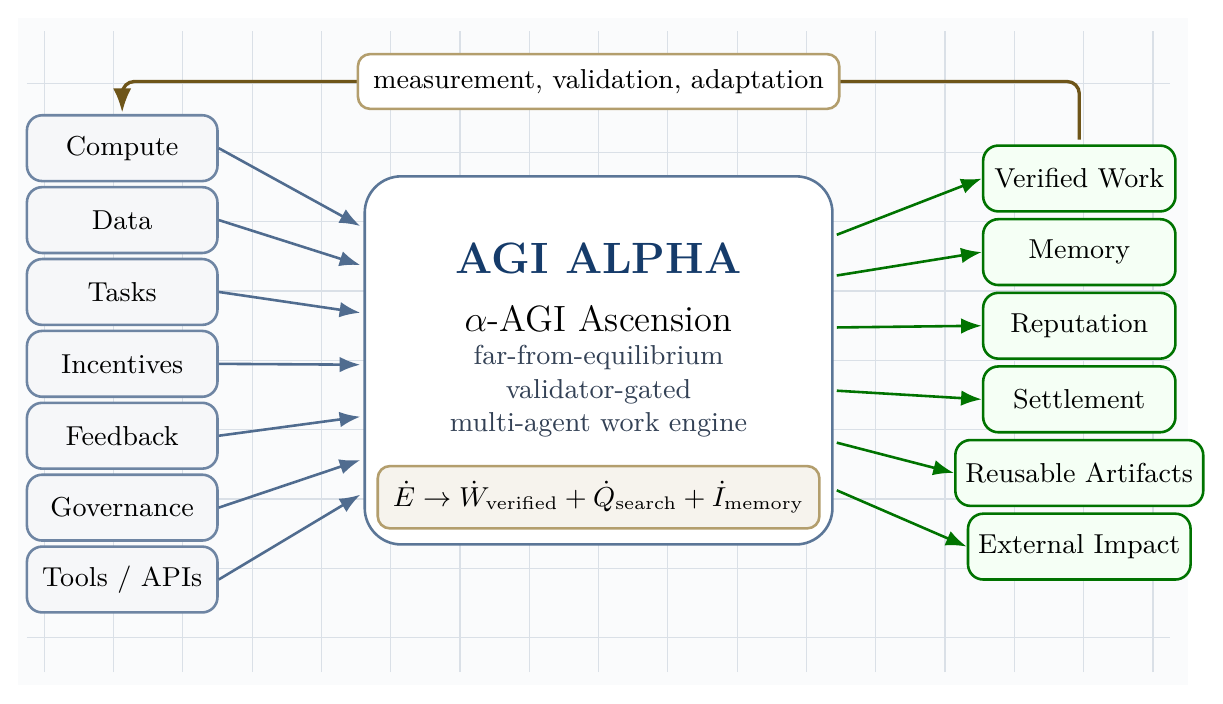
\includegraphics[width=0.95\textwidth,height=\textheight]{figures_png/figure1_system_architecture.png}
\caption{Open-system architecture of organized agentic complexity.
Continuous inflows enter the AGI ALPHA core and are converted into
verified work, memory, reputation, settlement, reusable artifacts, and
external impact under measurement, validation, and adaptation.}
\end{figure}

The architecture figure compresses the central systems claim: α-AGI
Ascension is sustained organization under regulated inflow, not isolated
one-shot inference.

\section{Definitions}\label{definitions}

Let:

\[
\mathcal{A}=\{a_1,\ldots,a_N\}
\]

be a population of agents, and let:

\[
\mathcal{J}=\{j_1,\ldots,j_M\}
\]

be a stream of jobs. Each job is a tuple:

\[
j=(o,c,v,b,d,\rho)
\]

where \(o\) is the objective, \(c\) is the constraint set, \(v\) is the
validation criterion, \(b\) is the bounty or reward, \(d\) is the
deadline, and \(\rho\) is the risk class.

\textbf{AGI ALPHA} is defined here as the proposed runtime/protocol
layer that routes jobs, agents, tools, memory, proofs, incentives, and
governance into a coordinated work-producing system.

\textbf{α-AGI Ascension} is defined as the operating regime in which
heterogeneous agents form, execute, validate, and dissolve coalitions to
maximize verified impact under bounded risk.

Formally, Ascension requires:

\[
\frac{d}{dt}\mathbb{E}[V_{\text{verified}}] > 0
\]

while maintaining:

\[
\mathbb{E}[R_{\text{safety}}] \leq R_{\max}
\]

and productive swarm entropy:

\[
S_{\min}<S_{\text{swarm}}<S_{\max}.
\]

The lower entropy bound prevents rigid monoculture; the upper bound
prevents incoherent chaos.

\section{Related work}\label{related-work}

\subsection{Dissipative structures}\label{dissipative-structures}

Dissipative structures are ordered patterns that arise and persist far
from equilibrium through exchange with an environment. Prigogine's work
is the canonical foundation for this perspective {[}1{]}. The agentic
analogue is not metabolism in a biological sense; it is the use of
electricity, processors, networks, storage, data, tools, and validation
to sustain organized computation.

\subsection{Gibbs free energy}\label{gibbs-free-energy}

Classically, Gibbs free energy is:

\[
G=H-TS.
\]

At constant temperature and pressure, negative \(\Delta G\) indicates a
spontaneous direction of change, \(\Delta G=0\) indicates equilibrium,
and Gibbs free energy is associated with the useful non-expansion work
obtainable from a process under ideal conditions. OpenStax summarizes
these relationships and the role of coupled reactions in driving
otherwise unfavorable processes {[}2{]}. We use physical Gibbs energy
literally at the hardware layer and a Gibbs-like optimization functional
at the agentic coordination layer.

\subsection{Statistical mechanics and maximum
entropy}\label{statistical-mechanics-and-maximum-entropy}

Jaynes' information-theoretic formulation of statistical mechanics
frames probability distributions as maximum-entropy inferences under
constraints {[}3{]}. This is useful for agent swarms because exact
microstate tracking is intractable. We model the swarm by distributions
over possible configurations and monitor macro-observables such as
entropy, expected verified value, risk, cost, and coalition stability.

\subsection{Hamiltonian multi-agent
learning}\label{hamiltonian-multi-agent-learning}

Bailey and Piliouras show a formal connection between multi-agent
learning in network zero-sum games and Hamiltonian dynamics {[}4{]}.
This matters because a system of interacting learners can cycle rather
than converge. α-AGI must therefore combine Hamiltonian exploration with
dissipative convergence into validated work.

\subsection{LLM-based multi-agent
systems}\label{llm-based-multi-agent-systems}

Recent surveys of LLM-based multi-agent systems emphasize profiling,
communication, workflow design, infrastructure, security, benchmarking,
and scalability challenges {[}5-7{]}. These surveys support a core claim
of this paper: large-scale multi-agent intelligence is not merely a
matter of increasing the number of agents. The difficult problems are
orchestration, communication, grounding, role specialization, credit
assignment, validation, and governance.

\subsection{Learned coordination
substrates}\label{learned-coordination-substrates}

Two recent coordinator papers sharpen the multi-agent coordination
problem. Conductor shows that a language model can learn to output
natural-language subtasks, worker assignments, and access lists, thereby
learning not only model routing but also prompt-engineered decomposition
and communication topology; randomized worker-pool training supports
adaptation to cost and availability constraints, while recursive
topologies create a bounded test-time scaling axis {[}69{]}. TRINITY
shows the complementary extreme: a compact language model plus a very
small routing head can select model/role pairs across turns, using a
Thinker/Worker/Verifier grammar, hidden-state representations, and
separable evolutionary optimization under low-signal terminal rewards
{[}24{]}. AGI ALPHA treats these works as scientific prior-art context,
not implementation dependencies: its coordination layer must learn over
real-work evidence states, bounded tools, validators, ledgers, memory,
settlement, and governance.

\subsection{Agentic deployment
practice}\label{agentic-deployment-practice}

Recent official and community guidance converges on a practical
principle: production agents require clear tools, guardrails, tracing,
orchestration, and escalation. Anthropic distinguishes workflows, where
code paths are predefined, from agents, where models dynamically direct
tool use and process control {[}10{]}. OpenAI's agent guidance
emphasizes model selection, tool design, guardrails, single-agent versus
multi-agent orchestration, manager patterns, decentralized handoffs, and
tracing {[}11{]}. MCP and related protocols are emerging as standard
ways to connect agents to external data and tools, but they also expand
the security boundary {[}12{]}.

\subsection{Risk management and agentic
security}\label{risk-management-and-agentic-security}

NIST's AI Risk Management Framework and the Generative AI Profile
provide lifecycle risk-management guidance for design, development, use,
and evaluation {[}8{]}. OWASP's Agentic AI Threats and Mitigations and
Securing Agentic Applications guidance emphasize threat modeling for
autonomous systems, including tool misuse, identity and privilege abuse,
memory risks, multi-agent propagation, and governance failures {[}9{]}.
These sources motivate the paper's insistence that maximum impact must
mean \textbf{verified bounded impact}, not unconstrained autonomy.

\section{Frontier synthesis: from coordination problem to sovereign
invention
system}\label{frontier-synthesis-from-coordination-problem-to-sovereign-invention-system}

The supplied corpus and the recent literature converge on one hard
problem: how to make many heterogeneous agents coordinate to maximum
useful effect without collapsing into waste, collusion, brittle
hierarchy, or unsafe autonomy. The strongest current answer is not a
single monolithic model. It is an institutionalized control stack that
combines evolved coordination, symbolic compression, persistent memory,
test-time learning, proof-bearing execution, and distributional safety.

Conductor is directly relevant because it demonstrates that
natural-language coordination can be learned: a coordinator can output
subtasks, worker assignments, and access relationships, learning not
only which model to call but what each worker should attempt and what
information it should see {[}69{]}. TRINITY supplies the complementary
lightweight lesson: coordination can be represented as a compact
evidence-state-to-action map, where hidden-state features from a small
model feed a tiny head that selects model/role pairs across Thinker,
Worker, and Verifier turns {[}24{]}. Multi-Agent Collaboration via
Evolving Orchestration reaches a related conclusion from a different
direction: static topologies scale poorly, while a learned orchestrator
can dynamically activate, sequence, and prune agents as task states
evolve {[}25{]}. The Era of Agentic Organization extends the same idea
into asynchronous thinking: an organizer assigns sub-queries, merges
intermediate knowledge, and can itself be optimized through
reinforcement learning {[}26{]}.

Planning and tool use require a second discipline: the LLM should not be
allowed to hallucinate the plan when a symbolic planner, executor, or
validator can do the logical work. DUPLEX restricts the LLM to
schema-guided information extraction and hands rigorous synthesis to a
PDDL planner, activating a slower reflective repair loop only after
planning failure {[}27{]}. AT\(^2\)PO adds the learning counterpart:
multi-turn agentic RL needs turn-level trees, entropy-guided
exploration, and turn-wise credit assignment because sparse terminal
rewards are too coarse for agentic action {[}28{]}.

Persistent agency and recursive improvement add a third layer. Sophia
frames a persistent agent as a System 3 wrapper over perception and
deliberation, maintaining narrative identity, long-horizon adaptation,
thought search, memory, and hybrid reward {[}29{]}. Self-play SWE-RL
shows that software agents can gather experience from real repositories
by injecting and repairing bugs specified by tests rather than relying
on human-written issues {[}30{]}. Huxley-Gödel Machine highlights a
subtle but essential distinction: an agent's current benchmark
performance is not the same as its self-improvement potential;
metaproductivity must be measured through the quality of descendants
{[}31{]}. ThetaEvolve shows how test-time learning can internalize
evolving strategies on open optimization problems instead of leaving all
progress in inference-only search {[}32{]}.

Artificial-life systems sharpen the thermodynamic analogy. The bacterial
flagellar motor illustrates that apparently mysterious living motion can
be explained as a physical motor driven by proton motive force and
molecular interactions, without invoking a special life force {[}33{]}.
Digital Ecosystems shows the computational analogue: multiple neural
cellular automata can compete, adapt online, and be steered toward
edge-of-chaos regimes where stable complexity emerges from local
interactions and continuous learning {[}34{]}.

Finally, the safety and economic literature argues that collective
capability must be governed distributionally. Distributional AGI Safety
explicitly addresses the patchwork hypothesis: AGI-level capability may
first appear through coordinated groups of sub-AGI agents, requiring
safeguards beyond individual-model alignment {[}35{]}. Virtual Agent
Economies similarly argues for proactively designed agent markets with
auctions, accountability, trust, safety, and steerability {[}36{]}.
Large Causal Models from LLMs, K-Dense Analyst, Synthetic Data RL,
DISCO, and ASI-Arch point to the scientific discovery frontier: causal
extraction, hierarchical scientific agents, task-defined RL, multimodal
molecular design, and autonomous architecture search all show how
agentic systems can transform knowledge into validated invention when
paired with execution and evaluation {[}37-41{]}.

\begin{figure}
\centering
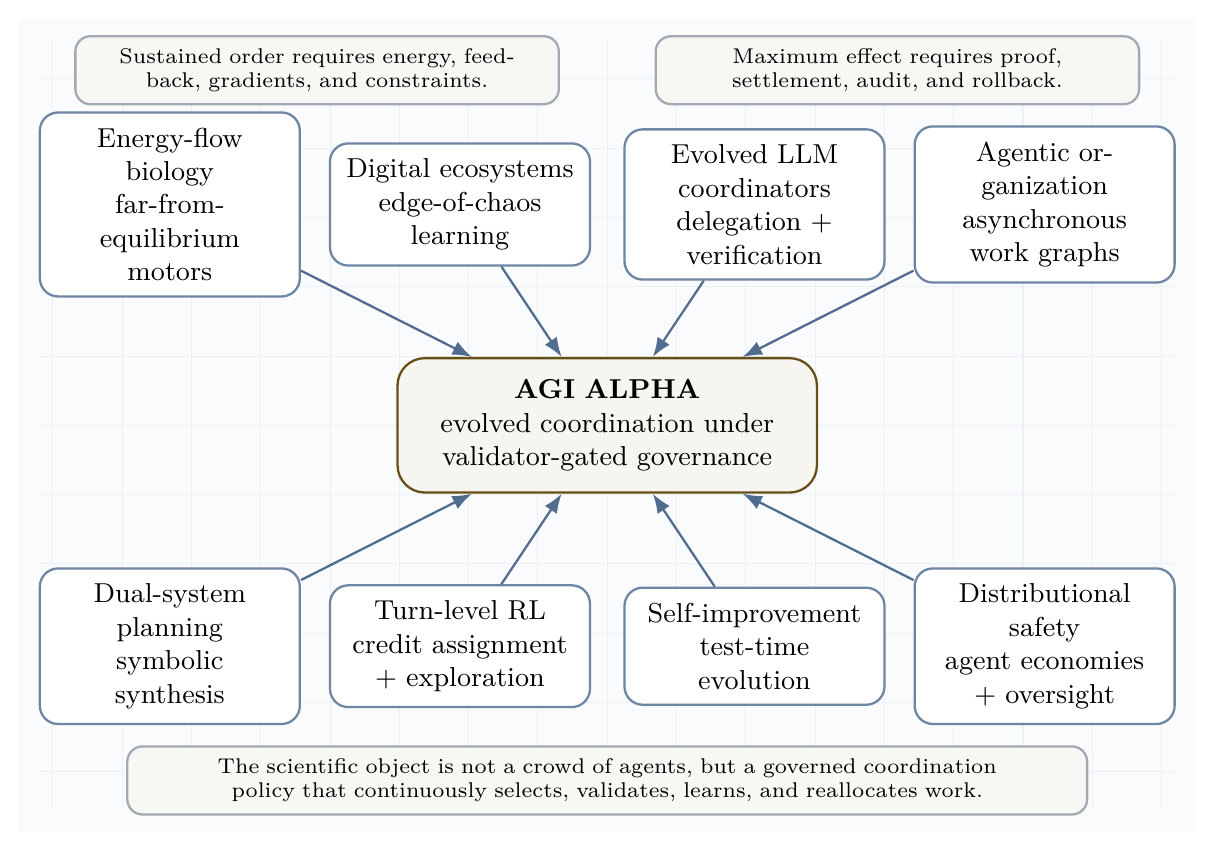
\includegraphics[width=0.96\textwidth,height=\textheight]{figures_png/figure10_frontier_synthesis_lattice.png}
\caption{Frontier synthesis lattice. Recent work across evolved
coordinators, digital ecosystems, dual-system planning, turn-level RL,
persistent agents, self-improvement, and distributional safety converges
on a single requirement: governed coordination under continuous inflow
and proof.}
\end{figure}

\begin{figure}
\centering
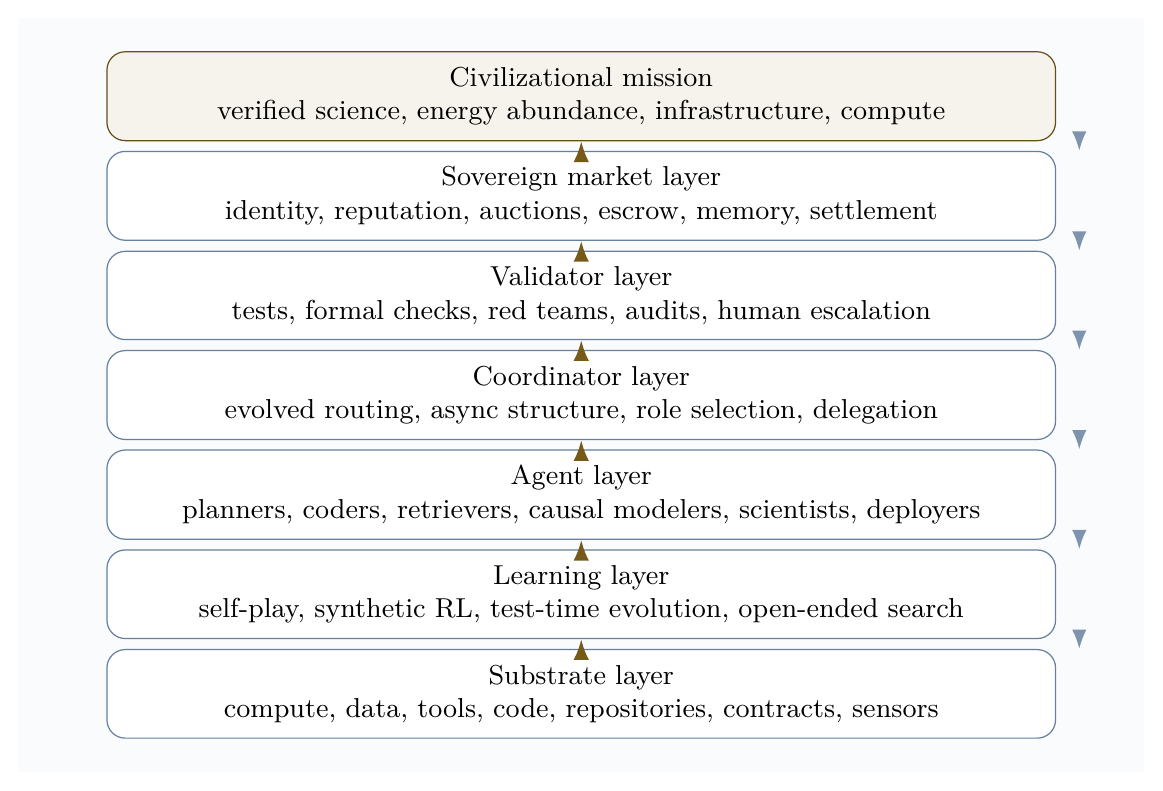
\includegraphics[width=0.96\textwidth,height=\textheight]{figures_png/figure11_sovereign_invention_stack.png}
\caption{Sovereign invention governance stack. The stack connects
continuous substrates to learning, agents, evolved coordination,
validation, market settlement, and civilizational mission while feedback
flows downward through policy, risk controls, and audit.}
\end{figure}

The resulting doctrine is a scientific operating principle:

\textbf{Operating principle.} Maximum useful effect = evolved coordination + formal verification + experience-grounded learning + value-relevant planning + recursive learning + distributional governance.

This principle reframes the central economic vision. A superhuman
invention engine is not best understood as a single automation product.
It is a compounding institutional asset: the owner-operator uses it to
generate proofs, tools, science, infrastructure, energy capacity, and
more compute, while external access is mediated through jobs, markets,
and validator-gated settlement.

\subsection{Frontier implication
matrix}\label{frontier-implication-matrix}

The following matrix translates the supplied frontier corpus into design
requirements for AGI ALPHA. The point is not to cite every item as proof
of achieved AGI. The point is to extract the strongest operational
pattern from each line of research and convert it into an engineering
control.

\begin{longtable}[]{@{}
  >{\raggedright\arraybackslash}p{(\columnwidth - 4\tabcolsep) * \real{0.3333}}
  >{\raggedright\arraybackslash}p{(\columnwidth - 4\tabcolsep) * \real{0.3333}}
  >{\raggedright\arraybackslash}p{(\columnwidth - 4\tabcolsep) * \real{0.3333}}@{}}
\toprule\noalign{}
\begin{minipage}[b]{\linewidth}\raggedright
Frontier signal
\end{minipage} & \begin{minipage}[b]{\linewidth}\raggedright
Core lesson
\end{minipage} & \begin{minipage}[b]{\linewidth}\raggedright
AGI ALPHA design implication
\end{minipage} \\
\midrule\noalign{}
\endhead
\bottomrule\noalign{}
\endlastfoot
Evolved LLM coordination & Coordination can be optimized directly, not
merely hand-written. & Learn a coordinator that selects roles, models,
tools, validators, and stopping rules under budget. \\
Agentic organization & Work graphs can be asynchronous, dynamic, and
learned. & Route jobs as evolving work graphs rather than static chains
of agents. \\
Dual-system planning & LLMs should ground semantics; symbolic planners
should enforce logic when stakes are high. & Separate semantic
extraction from plan synthesis, validation, and settlement. \\
Turn-level agentic RL & Sparse terminal rewards are insufficient for
multi-turn work. & Assign credit and policy updates at the turn,
tool-call, and subgoal level. \\
Persistent agents & Long-lived agents need memory, self-models, and
procedure updates. & Treat identity, lineage, reputation, and memory as
state variables, not chat history. \\
Self-play software RL & Agents can create training experiences from real
codebases through test-specified perturbations. & Use sandboxed
self-play only when tasks are externally checkable by tests, proofs, or
validators. \\
Test-time evolution & Search should become learning when repeated task
families reveal reusable structure. & Convert successful traces into
updateable routing priors, skills, and symbolic rules. \\
Artificial-life ecosystems & Local competition plus learning can
stabilize edge-of-chaos complexity. & Use bounded competition, niches,
gradients, and perturbation tests to discover robust agent ecologies. \\
Distributional AGI safety & AGI-level capability may emerge from
populations before a monolith. & Govern the swarm economy itself:
markets, audits, reputation, identity, and containment. \\
Scientific discovery agents & Causal extraction, bio-design, data
science, and architecture search become agentic workflows. & Build
invention loops that couple hypothesis, execution, verification,
compression, and reinvestment. \\
Web/tool agents & Browser and API actuation turn reasoning into external
action. & Treat tools as risk-bearing actuation channels with schemas,
scopes, logs, and reversible modes. \\
ARC-style abstraction & Extreme generalization favors symbolic
compression and deliberate test-time search. & Reward compact rules that
survive held-out tests, not persuasive explanations alone. \\
\end{longtable}

\subsection{Coordination as the central
prize}\label{coordination-as-the-central-prize}

The hard problem is not merely to make agents numerous. The hard problem
is to make them \textbf{coordinate to maximum useful effect}. In this
paper, maximum effect is not raw throughput. It is verified work under
bounded risk, low waste, recoverable failures, and compounding memory:

\[
\pi^*_{\text{coord}}
=
\arg\max_{\pi}
\mathbb{E}\left[
V_{\text{verified}}
-
\lambda C_{\text{compute}}
-
\rho R_{\text{safety}}
-
\kappa C_{\text{coordination}}
-
\mu U_{\text{unknown}}
\right].
\]

The frontier literature implies that this policy must be
\textbf{evolved}, \textbf{tested}, and \textbf{audited}. Hand-designed
org charts are too brittle. Pure self-play is too easily untethered from
human-useful objectives outside two-player zero-sum games. Static swarms
are too expensive. Single-model planners are too hallucination-prone.
The strong answer is a validator-gated coordination policy that learns
which agent should think, which should act, which should verify, when to
stop, and when to escalate.

This gives a sharper version of the AGI ALPHA thesis:

\[
\boxed{
\text{Ascension is not many agents. Ascension is learned coordination under proof.}
}
\]

\subsection{Learned Coordination Substrates: Conductor, TRINITY, and AGI
ALPHA}\label{learned-coordination-substrates-conductor-trinity-and-agi-alpha}

The new frontier is not merely multi-agent prompting. It is
\emph{learned coordination}: a policy that decides which agents should
exist for a task, what each agent should do, what each agent may see,
which tools each agent may use, how long the workflow may run, which
validators terminate the process, and what evidence is written back into
memory.

\textbf{Conductor lesson.} Conductor shows that a language model can
learn to orchestrate other language models by emitting natural-language
subtasks, worker assignments, and access lists {[}69{]}. The key
contribution is not only routing among workers. It is learning a
prompt-engineered decomposition and communication topology: which worker
should plan, which should execute, which intermediate outputs should be
visible, and how much compute a task deserves. Randomized worker-pool
training supports adaptation to user cost and availability constraints,
and recursive topologies create a bounded test-time scaling axis.

Mapped into AGI ALPHA, the Conductor-style lesson becomes:

\textbf{AGI ALPHA mapping:} task manifest -\textgreater{} role graph
-\textgreater{} subtask prompts -\textgreater{} access graph
-\textgreater{} worker calls -\textgreater{} validator gate
-\textgreater{} evidence bundle.

\textbf{TRINITY lesson.} TRINITY shows that a lightweight coordinator
can use hidden-state representations from a compact language model plus
a tiny head to select agents and roles across multiple turns {[}24{]}.
Its Thinker/Worker/Verifier protocol is a minimal learned coordination
grammar: one role decomposes, one role executes, one role checks and
terminates. Its sep-CMA-ES training result is important because
coordination often has low-signal terminal rewards, tight evaluation
budgets, and weakly coupled parameters; in that regime, derivative-free
evolutionary optimization can be more practical than standard policy
gradients or supervised imitation. TRINITY's hidden-state separability
analysis also suggests a diagnostic rule for AGI ALPHA: measure
task/agent separability before choosing whether to use a heuristic
router, a language workflow router, a lightweight representation router,
an evolutionary coordinator, or a hybrid.

Mapped into AGI ALPHA, the TRINITY-style lesson becomes:

\textbf{AGI ALPHA mapping:} evidence state -\textgreater{} lightweight
routing head -\textgreater{} role assignment -\textgreater{}
validator-terminated workflow.

\textbf{AGI ALPHA synthesis.} Conductor and TRINITY primarily
demonstrate LLM-to-LLM coordination on reasoning benchmarks. AGI ALPHA
must extend the same lesson into real work: tools, APIs, code execution,
browsers, databases, scientific workflows, policy-bound actions,
validator gates, safety ledgers, cost ledgers, settlement, memory, and
governance. Its routing decisions are judged not by conversational
elegance but by externally verified work, cost, risk, reproducibility,
lineage, and settlement.

\begin{figure}
\centering

\includegraphics[width=0.96\textwidth,height=\textheight]{figures_png/figure18_learned_coordination_substrates.png}
\caption{Learned coordination substrates. Conductor-style
natural-language workflow coordination and TRINITY-style lightweight
role routing become AGI ALPHA-native proof-conditioned orchestration
over tools, validators, ledgers, memory, and settlement.}
\end{figure}

\subsubsection{AGI ALPHA-native method
family}\label{agi-alpha-native-method-family}

The following method names are AGI ALPHA-native and commercially
independent. They are inspired by the coordination principle of
Conductor and TRINITY, but they do not depend on their code, prompts,
weights, figures, role prompts, exact training recipes, or
implementation details.

\begin{longtable}[]{@{}
  >{\raggedright\arraybackslash}p{(\columnwidth - 2\tabcolsep) * \real{0.5000}}
  >{\raggedright\arraybackslash}p{(\columnwidth - 2\tabcolsep) * \real{0.5000}}@{}}
\toprule\noalign{}
\begin{minipage}[b]{\linewidth}\raggedright
Method
\end{minipage} & \begin{minipage}[b]{\linewidth}\raggedright
Definition
\end{minipage} \\
\midrule\noalign{}
\endhead
\bottomrule\noalign{}
\endlastfoot
Proof-Conditioned Orchestration & Routing conditioned on task manifest,
prior evidence bundles, validator availability, cost, risk, and expected
proof quality. \\
Evidence-State Coordinator & A lightweight router whose input state is
the current evidence graph: task, trace, artifacts, test results, costs,
risks, memory, and validator outcomes. \\
Validator-Terminated Role Graphs & Learned role graphs whose stopping
condition is an external validator, formal check, policy gate, or
explicit escalation rule. \\
Proof-Gradient Routing & Routing updates that move probability mass
toward agents and topologies with higher verified value per unit cost
and lower false-acceptance risk. \\
Coordination Fitness Landscapes & Empirical landscapes over
agent-role-tool-validator combinations, learned from accepted and
rejected evidence bundles. \\
Recursive Audit Routing & Bounded recursion in which a router can call a
critique/router layer only under budget, depth, and validator
constraints. \\
Capability Complementarity Atlas & A memory map of which agents, tools,
and roles complement or interfere with one another across task
families. \\
Evidence-to-Policy Compression & Compression of traces, failures, and
validator reports into reusable routing priors, contracts, and safety
rules. \\
Tool-Bounded Role Contracts & Role definitions that include tool scopes,
data access, budget, allowed actions, prohibited actions, and validator
obligations. \\
Budgeted Constellation Search & Search over agent constellations under
token, dollar, latency, risk, and validator budgets. \\
\end{longtable}

\subsubsection{Formal comparison: Conductor, TRINITY, and AGI
ALPHA}\label{formal-comparison-conductor-trinity-and-agi-alpha}

\begin{longtable}[]{@{}
  >{\raggedright\arraybackslash}p{(\columnwidth - 6\tabcolsep) * \real{0.2500}}
  >{\raggedright\arraybackslash}p{(\columnwidth - 6\tabcolsep) * \real{0.2500}}
  >{\raggedright\arraybackslash}p{(\columnwidth - 6\tabcolsep) * \real{0.2500}}
  >{\raggedright\arraybackslash}p{(\columnwidth - 6\tabcolsep) * \real{0.2500}}@{}}
\toprule\noalign{}
\begin{minipage}[b]{\linewidth}\raggedright
Dimension
\end{minipage} & \begin{minipage}[b]{\linewidth}\raggedright
Conductor
\end{minipage} & \begin{minipage}[b]{\linewidth}\raggedright
TRINITY
\end{minipage} & \begin{minipage}[b]{\linewidth}\raggedright
AGI ALPHA
\end{minipage} \\
\midrule\noalign{}
\endhead
\bottomrule\noalign{}
\endlastfoot
Coordination representation & Natural-language workflow with subtasks,
worker ids, and access lists. & Hidden-state representation plus small
head over agent-role actions. & Evidence-state graph over task, agents,
tools, validators, memory, ledgers, settlement, and governance. \\
Learning method & Reinforcement learning over executed workflows. &
Evolutionary optimization of a lightweight coordinator. & Commercially
independent router family: heuristic, language, representation,
evolutionary, RL, and hybrid proof-conditioned routers. \\
Role system & Flexible natural-language subtasks and worker assignments.
& Thinker / Worker / Verifier tri-role grammar. & Tool-bounded role
contracts: planner, executor, retriever, simulator, validator, critic,
auditor, deployer, settlement agent. \\
Worker-pool adaptation & Randomized worker-pool training for cost and
availability constraints. & Selects among a pool of LLMs and roles. &
Capability complementarity atlas plus budgeted constellation search over
agents, tools, validators, and policies. \\
Recursion / test-time scaling & Recursive topology allows bounded calls
to the coordinator itself. & Multi-turn protocol with bounded turn
budget. & Recursive audit routing under depth, cost, risk, validator,
and escalation constraints. \\
Validation & Benchmark correctness after workflow execution. & Verifier
role and terminal benchmark reward. & External validator gates: tests,
formal checks, simulations, audits, market settlement, human expert
review, and real-world outcomes. \\
Evidence trace & Workflow trace and benchmark result. & Multi-turn
transcript and terminal score. & Machine-readable evidence bundle:
routing record, tool trace, artifacts, validation, cost, risk,
settlement, provenance, lineage. \\
Tool actuation & Primarily LLM-to-LLM benchmark workflows. & Primarily
LLM-to-LLM benchmark workflows. & Bounded tools, APIs, code, browser,
database, scientific workflow, and protocol-native job execution. \\
Safety controls & Benchmark-format constraints. & Turn budget and
verifier termination. & Least privilege, policy gates, safety ledger,
reversible actions, escalation, auditability, and governance. \\
Settlement / reputation & Not the central object. & Not the central
object. & Proof-based settlement, reputation, credit assignment, and
future routing probability. \\
Commercial independence & Prior-art inspiration only. & Prior-art
inspiration only. & Independent terminology, architecture, evidence
memory, safety-control layer, and settlement mechanism. \\
\end{longtable}

\subsubsection{Router family}\label{router-family}

The Hamiltonian router remains useful as the simplest interpretable
baseline, but it is no longer the only routing model. AGI ALPHA defines
a router family:

\begin{longtable}[]{@{}
  >{\raggedright\arraybackslash}p{(\columnwidth - 2\tabcolsep) * \real{0.5000}}
  >{\raggedright\arraybackslash}p{(\columnwidth - 2\tabcolsep) * \real{0.5000}}@{}}
\toprule\noalign{}
\begin{minipage}[b]{\linewidth}\raggedright
Router
\end{minipage} & \begin{minipage}[b]{\linewidth}\raggedright
Description
\end{minipage} \\
\midrule\noalign{}
\endhead
\bottomrule\noalign{}
\endlastfoot
R0: Heuristic Hamiltonian router & Hand-specified
free-energy/Hamiltonian scorer over cost, risk, complementarity, and
expected verified value. \\
R1: Natural-language workflow router & Generates role graph, subtask
prompts, access graph, and worker calls in natural language. \\
R2: Evidence-state lightweight router & Maps evidence-state features to
agent-role-tool-validator choices with a compact head. \\
R3: Evolutionary coordinator & Optimizes routing parameters by
derivative-free search under sparse terminal validator rewards. \\
R4: Reinforcement-learned coordinator & Learns workflow decisions from
validator rewards, tool outcomes, and cost/risk penalties. \\
R5: Hybrid router & Selects R0-R4 by task family, cost, risk, validator
availability, separability diagnostics, and evidence density. \\
\end{longtable}

Every router must output:

\begin{enumerate}
\def\labelenumi{\arabic{enumi}.}
\tightlist
\item
  selected agents;
\item
  role assignments;
\item
  subtask prompts;
\item
  access graph;
\item
  tool permissions;
\item
  budget;
\item
  validator set;
\item
  stopping rule;
\item
  escalation rule.
\end{enumerate}

A task \(j\) with evidence state \(e_t\) is routed by:

\[
R_k(e_t,j)\rightarrow(A,\rho,S,\Gamma_T,B,V_{set},\tau_{stop},\tau_{esc}),
\]

where \(A\) is the selected constellation, \(\rho\) are role contracts,
\(S\) are subtasks, \(\Gamma_T\) is the access/tool graph, \(B\) is the
budget, \(V_{set}\) is the validator set, and \(\tau_{stop},\tau_{esc}\)
are stopping and escalation rules.

The hybrid router is promoted only when evidence supports it:

\[
R^*(j)=\arg\max_{R_k}\;\mathbb{E}[D_{\mathrm{real}}\mid j,R_k]-\lambda C-\rho R-\kappa O.
\]

\subsubsection{Router-selection decision rule
example}\label{router-selection-decision-rule-example}

The router family is operational, not merely taxonomic. AGI ALPHA
should choose the simplest router that can satisfy the task's structure,
validator, budget, and risk constraints.

\begin{itemize}
\tightlist
\item
  \textbf{Choose R0} when the task is low-risk, well-understood, and
  historical evidence is sparse; R0 is the interpretable Hamiltonian
  baseline, not the primary long-run model.
\item
  \textbf{Choose R1} when the task requires open-ended decomposition,
  prompt-engineered subtasks, or flexible communication topology across
  heterogeneous agents.
\item
  \textbf{Choose R2} when evidence-state features are linearly or
  compactly separable by task family, agent capability, or role fitness,
  and low-latency routing is more valuable than expressive workflow
  generation.
\item
  \textbf{Choose R3} when rewards are sparse, terminal, noisy, or
  expensive to evaluate, and derivative-free search can discover
  coordination policies without dense labels.
\item
  \textbf{Choose R4} when the domain is stable enough to accumulate many
  validator-labeled episodes and reinforcement learning can optimize
  long-horizon tradeoffs over tool use, cost, risk, and success.
\item
  \textbf{Choose R5} for mixed, high-value, or high-risk work where task
  structure, validator availability, cost, safety class, and evidence
  density require a hybrid router chosen at run time.
\end{itemize}

A practical decision policy is:

\[
R_{\text{select}}(j)=\begin{cases}
R0, & \text{low risk, sparse evidence, simple validator};\\
R1, & \text{open-ended decomposition or natural-language workflow design};\\
R2, & \text{separable evidence state and tight latency/cost budget};\\
R3, & \text{sparse terminal reward or low-SNR validator signal};\\
R4, & \text{dense replay data and stable task distribution};\\
R5, & \text{mixed or high-impact task requiring proof-conditioned arbitration}.
\end{cases}
\]

In all cases, promotion from R0 to a learned router requires evidence
bundles showing higher \(D_{\mathrm{real}}\) under equal model, tool, and
budget constraints.

\subsubsection{Strict novelty relative to learned-coordination prior art}\label{strict-novelty-relative-to-learned-coordination-prior-art}

This paper does not claim that AGI ALPHA invents learned LLM coordination from scratch. The strict novelty claim is the \textbf{full-stack organizational substrate}: learned routing is integrated with bounded tools, external validators, machine-readable evidence bundles, cost and safety ledgers, memory graphs, proof-based settlement, reputation updates, and governance. Conductor and TRINITY show that coordination itself can be learned in benchmark-centric LLM collaboration. AGI ALPHA's contribution is to lift learned coordination into a validator-gated, commercially deployable work system where routing decisions are judged by externally verified artifacts, reproducible traces, real-task cost, safety outcomes, and future routing improvement.

\subsubsection{Commercial independence}\label{commercial-independence}

Conductor and TRINITY are cited as frontier demonstrations that
coordination itself can be learned. AGI ALPHA does not depend on their
code, weights, prompts, figures, role prompts, exact training recipes,
data, or proprietary implementation details. AGI ALPHA develops its own
commercially independent coordination substrate, validator architecture,
routing state, evidence memory, safety-control layer, cost/risk
accounting, settlement mechanism, and governance interface.

\subsubsection{State-of-the-art positioning and
caution}\label{state-of-the-art-positioning-and-caution}

The state-of-the-art lesson from Conductor and TRINITY is that learned
coordination can beat manual scaffolding. The AGI ALPHA thesis is that
learned coordination must now be lifted from benchmark-only LLM
collaboration into validator-gated real-world work systems. The novel
contribution claimed here is not that AGI ALPHA invents learned
LLM-to-LLM coordination from scratch; Conductor and TRINITY are cited
precisely because they show that coordination itself can be learned. AGI
ALPHA's commercially independent contribution is the \textbf{full-stack
organizational generalization}: routing plus bounded tools, external
validators, machine-readable evidence bundles, safety and cost ledgers,
memory, reputation, settlement, governance, and real-task promotion rules
in one substrate. Conductor and TRINITY optimize benchmark
collaboration; AGI ALPHA specifies the institutional layer needed to turn
learned coordination into auditable machine labor.

AGI ALPHA is therefore \textbf{SOTA-aligned as a research program and
architecture}. It becomes \textbf{empirically SOTA} only if its
proof-conditioned router beats Conductor-style, TRINITY-style,
single-agent, fixed-workflow, and unstructured-swarm baselines on real
tasks under equal model, tool, and budget constraints with zero critical
safety violations and reproducible evidence bundles.

\subsection{Experience-Grounded Coordination: AGI ALPHA in the Era of
Experience}\label{experience-grounded-coordination-agi-alpha-in-the-era-of-experience}

Silver and Sutton's \emph{Welcome to the Era of Experience} argues that
human-generated data is approaching limits in frontier domains and that
future agents will improve primarily through experience generated by
acting in environments, observing consequences, receiving grounded
rewards, and planning over long streams of interaction {[}70{]}. The
paper identifies four dimensions that matter for future agents: long
streams of experience, rich grounded actions and observations, grounded
rewards, and planning or reasoning over experience.

This section also explicitly anchors the experience layer in standard
reinforcement-learning concepts from Sutton and Barto's \emph{Reinforcement
Learning: An Introduction}, including value estimation from experience,
model-based planning, temporal-difference learning, Dyna-style learning from
real and simulated experience, and options as temporal abstractions {[}71{]}.
AGI ALPHA translates those concepts into organizational infrastructure:
evidence streams become the experience base, world models predict
consequences of agent/tool actions, temporal options become reusable
validator-bounded workflows, and governance controls which reward signals
may update production policy.

AGI ALPHA adopts this as conceptual inspiration and prior-art context
only. The scientific implication is decisive: AGI ALPHA should not
merely coordinate agents across isolated tasks. It should generate,
record, validate, compress, and learn from experience streams. Evidence
bundles are therefore not just audit logs. They are the training
substrate for future routing, world modeling, reward calibration, safety
policy, reputation, settlement, and governance.

\begin{longtable}[]{@{}
  >{\raggedright\arraybackslash}p{(\columnwidth - 2\tabcolsep) * \real{0.5000}}
  >{\raggedright\arraybackslash}p{(\columnwidth - 2\tabcolsep) * \real{0.5000}}@{}}
\toprule\noalign{}
\begin{minipage}[b]{\linewidth}\raggedright
Era-of-experience dimension
\end{minipage} & \begin{minipage}[b]{\linewidth}\raggedright
AGI ALPHA translation
\end{minipage} \\
\midrule\noalign{}
\endhead
\bottomrule\noalign{}
\endlastfoot
Streams of experience & Long-lived task, job, tool, validator,
settlement, incident, and delayed-outcome streams. \\
Grounded actions and observations & Bounded tools, APIs, code execution,
browsers, databases, sensors, simulations, lab interfaces, and
protocol-native actions. \\
Grounded rewards & Validator outcomes, test results, user outcomes,
scientific measurements, cost, safety, latency, reproducibility, market
settlement, and delayed real-world outcomes. \\
Planning and reasoning over experience & World models, consequence-aware
routing, temporal option registries, evidence-to-policy compression, and
sandbox-to-real escalation planning. \\
\end{longtable}

\begin{figure}
\centering

\includegraphics[width=0.96\textwidth,height=\textheight]{figures_png/figure19_experience_grounded_machine_labor.png}
\caption{From human data to experience-grounded machine labor.
Human-data AI imitates short human examples; experience-grounded agents
learn from action, observation, reward, and world models; AGI ALPHA
converts job/tool/validator interactions into governed experience
streams for future routing and settlement.}
\end{figure}

\subsubsection{Experience tuple and sovereign experience
stream}\label{experience-tuple-and-sovereign-experience-stream}

An AGI ALPHA experience event is defined as:

\[
e_t=(s_t,a_t,o_{t+1},r_t,v_t,c_t,\rho_t,m_t)
\]

where:

\begin{itemize}
\tightlist
\item
  \(s_t\) is the task/evidence state;
\item
  \(a_t\) is the agent, tool, workflow, or governance action;
\item
  \(o_{t+1}\) is the next observation, tool result, test result,
  simulator output, user outcome, market event, or scientific
  measurement;
\item
  \(r_t\) is a grounded reward signal;
\item
  \(v_t\) is a validator decision;
\item
  \(c_t\) is the cost, latency, and resource ledger;
\item
  \(\rho_t\) is the risk and safety state;
\item
  \(m_t\) is the memory, reputation, settlement, and policy update.
\end{itemize}

The experience stream is:

\[
E_{0:T}=\{e_0,e_1,\ldots,e_T\}.
\]

This matters because isolated task success can be misleading. A patch
may pass immediate tests but fail under delayed deployment. A browser
workflow may satisfy a page-state evaluator while violating a policy. A
scientific design may score well in a proxy but fail a real assay. The
experience stream preserves the difference between immediate acceptance
and longer-run consequence.

\subsubsection{Sovereign Experience Control
Plane}\label{sovereign-experience-control-plane}

The decisive upgrade is to treat experience as first-class
infrastructure. A one-shot evidence bundle proves what happened in one
run; a sovereign experience stream preserves the ordered sequence of
runs from which future routers, validators, world models, option
policies, and governance weights can improve. This turns AGI ALPHA from
a task coordinator into an experience operating system for machine
labor.

The experience-control plane maintains four coupled state updates:

\[
M_{t+1}=U_M(M_t,e_t)
\]

\[
\Omega_{t+1}=U_\Omega(\Omega_t,r_t,v_t,\rho_t,\Pi_t)
\]

\[
M_{\phi,t+1}=U_\phi(M_{\phi,t},E_{0:t})
\]

\[
\pi_{t+1}=U_\pi\big(\pi_t,\mathrm{Compress}(E_{0:t}),M_{\phi,t+1},\Omega_{t+1}\big).
\]

Here \(M_t\) is operational memory, \(\Omega_t\) is the
reward-governance state, \(M_{\phi,t}\) is the world model, and
\(\pi_t\) is the router/policy state. The update rule is deliberately
separated into memory, reward governance, world modeling, and routing
because each subsystem has a different failure mode. Memory can be
poisoned, rewards can be gamed, world models can extrapolate
incorrectly, and routers can overfit to validator shortcuts. The control
plane therefore requires provenance, quarantine, replay, delayed-outcome
checks, and independent validator review before high-impact traces are
allowed to influence production routing.

\begin{figure}
\centering

\includegraphics[width=0.96\textwidth,height=\textheight]{figures_png/figure20_sovereign_experience_control_plane.png}
\caption{Sovereign experience control plane. Experience events turn
validator-gated work into a governed training substrate for reward
ledgers, memory graphs, world models, temporal options, and
router-family updates.}
\end{figure}

The key distinction is:

\begin{longtable}[]{@{}
  >{\raggedright\arraybackslash}p{(\columnwidth - 4\tabcolsep) * \real{0.3333}}
  >{\raggedright\arraybackslash}p{(\columnwidth - 4\tabcolsep) * \real{0.3333}}
  >{\raggedright\arraybackslash}p{(\columnwidth - 4\tabcolsep) * \real{0.3333}}@{}}
\toprule\noalign{}
\begin{minipage}[b]{\linewidth}\raggedright
Object
\end{minipage} & \begin{minipage}[b]{\linewidth}\raggedright
Function
\end{minipage} & \begin{minipage}[b]{\linewidth}\raggedright
Can update production policy?
\end{minipage} \\
\midrule\noalign{}
\endhead
\bottomrule\noalign{}
\endlastfoot
Evidence bundle & Immutable proof of a single run & No, not by itself \\
Experience event & Atomic
state-action-observation-reward-validation-cost-risk-memory tuple & Only
after provenance checks \\
Experience stream & Ordered sequence of events across jobs and cycles &
Yes, if replayable and validated \\
Reward ledger & Versioned consequence record & Yes, under governance
weights \\
World model & Predictive model of outcomes and risk & Yes, if calibrated
and monitored \\
Temporal option & Reusable validated macro-workflow & Yes, if bounded by
initiation, validation, termination, and risk class \\
\end{longtable}

The system's experience-grounded progress is measured over time, not by
a single impressive run:

\[
D_{\mathrm{experience}}(T)=
\frac{1}{T}\sum_{t=1}^{T}
\left[
\frac{V^{(t)}_{\mathrm{verified}}}{C^{(t)}_{\mathrm{tokens}}+C^{(t)}_{\mathrm{tool}}+C^{(t)}_{\mathrm{time}}}
\right]
(1-R^{(t)}_{\mathrm{critical}})
(1-O^{(t)}_{\mathrm{coord}})
(1-H^{(t)}_{\mathrm{reward}}),
\]

where \(H^{(t)}_{\mathrm{reward}}\) is the detected reward-hacking or
reward-provenance penalty. A claimed experience gain must show that
\(D_{\mathrm{experience}}(T)\) improves on held-out future tasks while
critical violations, reward hacking, and false acceptance do not
increase.


\subsubsection{Validator-reward
separation}\label{validator-reward-separation}

AGI ALPHA separates validators from rewards.

\begin{itemize}
\tightlist
\item
  Validators determine whether an artifact, action, or workflow is
  accepted for the current job.
\item
  Grounded rewards measure consequences across time, cost, safety,
  reproducibility, markets, sensors, tests, scientific assays, user
  outcomes, and delayed real-world feedback.
\item
  Human approval is useful but is not identical to truth, utility, or
  safety.
\item
  Immediate validator acceptance can be contradicted by long-run
  outcomes.
\item
  Delayed grounded outcomes must be attributed back to prior agents,
  tools, prompts, policies, and routing decisions.
\end{itemize}

Thus the system tracks both:

\[
v_t=\mathrm{accept/reject/escalate}
\]

and:

\[
r_t=R(o_{t+1},c_t,\rho_t,\mathrm{delayed\ outcomes},\mathrm{governance\ weights}).
\]

This distinction protects AGI ALPHA from mistaking a narrow pass/fail
gate for a complete account of value, truth, safety, or long-run
usefulness.

\subsubsection{AGI ALPHA-native method
family}\label{agi-alpha-native-method-family}

These methods are AGI ALPHA-native and commercially independent. They
are inspired by the general scientific lesson that agents can learn from
grounded experience, but they do not depend on Silver/Sutton code,
figures, algorithms, training recipes, or proprietary artifacts.

\begin{longtable}[]{@{}
  >{\raggedright\arraybackslash}p{(\columnwidth - 2\tabcolsep) * \real{0.5000}}
  >{\raggedright\arraybackslash}p{(\columnwidth - 2\tabcolsep) * \real{0.5000}}@{}}
\toprule\noalign{}
\begin{minipage}[b]{\linewidth}\raggedright
Method
\end{minipage} & \begin{minipage}[b]{\linewidth}\raggedright
Definition and commercial-independence note
\end{minipage} \\
\midrule\noalign{}
\endhead
\bottomrule\noalign{}
\endlastfoot
Experience-Grounded Coordination & Routing conditioned on current task
state plus accumulated experience streams, not isolated prompts. \\
Sovereign Experience Streams & Institution-owned streams of task, tool,
validator, cost, risk, settlement, and delayed-outcome events. \\
Grounded Reward Ledger & Versioned accounting of rewards from tests,
simulations, markets, sensors, assays, user outcomes, safety, latency,
and reproducibility. \\
Validator-Reward Separation & Explicit separation between acceptance
gates and consequence-measuring rewards. \\
Experience-to-Policy Compression & Compression of repeated traces into
routing priors, validator policies, temporal options, and governance
updates. \\
Consequence-Aware Routing & Routing that predicts downstream cost,
safety, latency, validator failure, delayed outcome, and escalation
risk. \\
World-Model Risk Planning & Predictive modeling used before tool
escalation, external deployment, or high-risk scientific action. \\
Temporal Option Registry & Reusable macro-actions with initiation
conditions, workflow policy, validator, termination condition, risk
class, and lineage. \\
Bi-Level Reward Governance & Low-level grounded signals are weighted and
corrected by high-level policy, law, user feedback, institutional
priorities, and safety events. \\
Exploration Corridors & Bounded zones where agents may explore novel
actions, tools, or hypotheses under budget, sandbox, validator,
rollback, and quarantine constraints. \\
Delayed Outcome Attribution & Assignment of long-run outcomes back to
prior routing, tool, prompt, policy, and agent decisions. \\
Experience Quarantine and Replay & Isolation of suspicious, unsafe,
poisoned, or reward-hacking traces, followed by controlled replay before
learning from them. \\
\end{longtable}

\subsubsection{Grounded Reward Ledger and Bi-Level Reward
Governance}\label{grounded-reward-ledger-and-bi-level-reward-governance}

Low-level reward signals can come from unit tests, simulations, markets,
sensors, scientific assays, user outcomes, cost, latency, safety, and
reproducibility. These signals are powerful because they measure
consequences rather than only predicted human approval. They are also
dangerous because any single signal can be gamed.

AGI ALPHA therefore uses a governed reward functional:

\[
R_t^{\mathrm{AGI\ ALPHA}}
=
G_\omega\left(r_t^{\mathrm{tests}},r_t^{\mathrm{simulation}},r_t^{\mathrm{market}},r_t^{\mathrm{safety}},r_t^{\mathrm{cost}},r_t^{\mathrm{latency}},r_t^{\mathrm{reproducibility}},r_t^{\mathrm{human}},r_t^{\mathrm{delayed}}\right),
\]

where \(G_\omega\) is a versioned governance policy. The low level
optimizes grounded signals; the high level adjusts which signals matter,
how they are weighted, and when safety or law overrides apparent reward.
User feedback, legal constraints, incident reports, institutional
policy, and human concern signals provide top-level correction. This
makes reward design auditable and governable rather than an invisible
optimization target.

\subsubsection{World-model planning and consequence-aware
routing}\label{world-model-planning-and-consequence-aware-routing}

Experience streams support world models. This follows the standard reinforcement-learning idea that agents can improve by learning predictive models from experience and using those models for planning; AGI ALPHA reinterprets this as an auditable organizational mechanism rather than a single-agent algorithm {[}71{]}. AGI ALPHA defines:

\[
M_\phi(o_{t+1},r_t,\rho_{t+1}\mid s_t,a_t),
\]

where \(M_\phi\) predicts observations, reward, and future risk from a
state-action pair. Such models support consequence-aware routing,
delayed outcome prediction, safety forecasting, cost and latency
forecasting, validator failure prediction, scientific experiment
planning, sandbox-to-real escalation, rollback, and quarantine
decisions.

The router family becomes experience-aware:

\[
R_k(e_t,j,E_{0:T},M_\phi)\rightarrow(A,\rho,S,\Gamma_T,B,V_{set},\tau_{stop},\tau_{esc}),\qquad k\in\{0,1,2,3,4,5\}.
\]

A router should not merely ask which agent is best for the immediate
prompt. It should ask which constellation is most likely to produce
valid work after considering downstream validators, delayed outcomes,
cost, safety, and reversibility.

\subsubsection{Temporal option registry}\label{temporal-option-registry}

Long streams of experience make reusable temporal abstractions possible.
A validated workflow becomes an option or macro-action:

\[
\mathrm{Option}=(\mathcal{I},\pi_{workflow},V_{gate},\tau_{term},\rho_{risk},H_{evidence}).
\]

Here \(\mathcal{I}\) is the initiation condition, \(\pi_{workflow}\) is
the workflow policy, \(V_{gate}\) is the validator, \(\tau_{term}\) is
the termination condition, \(\rho_{risk}\) is the risk class, and
\(H_{evidence}\) is the evidence history. Examples include software
repair, benchmark execution, literature review, simulation, red-team
review, deployment rollback, and scientific experiment options. Temporal
abstraction matters because civilization-scale work is not a collection
of one-shot answers; it is the repeated reuse and improvement of
verified procedures.

\subsubsection{Anti-reward-hacking
controls}\label{anti-reward-hacking-controls}

Grounded rewards are necessary, but unsafe if treated as the only
objective. AGI ALPHA therefore requires reward provenance, reward
versioning, counterfactual reward audits, adversarial reward tests,
delayed-outcome checks, independent validator review, safety overrides,
rollback and quarantine, human concern signals, reward-model incident
reports, and replay before learning from suspicious traces.

The system is allowed to learn from experience only when the experience
remains traceable, replayable, and governed.

\subsubsection{Commercial independence}\label{commercial-independence}

Silver and Sutton are cited as conceptual inspiration and prior-art
context for the shift from human-data-centric systems toward
experience-grounded agents. AGI ALPHA does not depend on their code,
figures, algorithms, training recipes, terminology beyond ordinary
citation, or implementation details. AGI ALPHA defines its own
commercially independent experience tuple, evidence-stream architecture,
grounded reward ledger, validator-reward separation, world-model
planning interface, temporal option registry, router-family extension,
safety controls, and settlement mechanism.


\subsection{Planning with Learned Organizational Models: MuZero-Inspired
AGI ALPHA without Implementation
Dependence}\label{planning-with-learned-organizational-models-muzero-inspired-agi-alpha-without-implementation-dependence}

The frontier lesson from MuZero is not generic model-based reinforcement
learning. Its decisive scientific contribution is \textbf{value-relevant
planning}: learning an abstract latent model that predicts the
quantities needed for search - reward, policy, and value - without
requiring reconstruction of the full environment state {[}72{]}. AGI
ALPHA adopts this as inspiration only and translates it into a
commercially independent planning substrate over organizational
evidence.

For AGI ALPHA, the environment is not a board game or Atari emulator. It
is a real work system: agents, jobs, tools, APIs, code repositories,
browsers, databases, validators, costs, risks, memory, settlement, and
governance. A useful planner therefore need not reconstruct the full
world. It must predict the consequences relevant to bounded work: which
organizational action is likely to produce verified value, at what cost,
under which validator, with what safety and settlement consequences.

\subsubsection{AGI ALPHA-native method
family}\label{agi-alpha-native-method-family}

The following methods are AGI ALPHA-native. They are inspired by the
scientific principle of value-relevant learned planning, but do not
reuse MuZero code, pseudocode, figures, hyperparameters, implementation
details, model weights, training recipes, or architecture.

\begin{longtable}[]{@{}
  >{\raggedright\arraybackslash}p{(\columnwidth - 2\tabcolsep) * \real{0.5000}}
  >{\raggedright\arraybackslash}p{(\columnwidth - 2\tabcolsep) * \real{0.5000}}@{}}
\toprule\noalign{}
\begin{minipage}[b]{\linewidth}\raggedright
Method
\end{minipage} & \begin{minipage}[b]{\linewidth}\raggedright
AGI ALPHA definition
\end{minipage} \\
\midrule\noalign{}
\endhead
\bottomrule\noalign{}
\endlastfoot
Proof-Equivalent Organizational Models & Learned abstract models whose
predictions are sufficient for choosing actions that improve verified
work, not for reconstructing the full external world. \\
Latent Evidence Dynamics & Transition models over compressed evidence
states, validator histories, cost ledgers, risk ledgers, and memory
updates. \\
Validator-Aware Tree Planning & Bounded search over organizational
actions constrained by permissions, budget, risk class, validator
availability, and escalation rules. \\
Search-Improved Routing & Router policies improved by tree search
targets generated from learned organizational models. \\
Evidence Reanalyze & Revisit old evidence bundles with newer routers and
world models to generate fresher value, policy, validator-risk, and cost
targets while preserving provenance. \\
ProofZero Planning Layer & AGI ALPHA's native planning layer for
value-relevant organizational search over proof-bearing work states. \\
Cost-Risk-Value Backup & Backups that combine predicted reward, future
verified value, cost, latency, safety, and validator failure risk. \\
Abstract Work-State Planning & Planning in latent work states that
preserve decision-relevant evidence rather than full environment
reconstructions. \\
Policy/Value/Reward Heads for Machine Labor & Predictive heads for
routing policy, grounded reward, downstream verified value, and
validator/safety/cost outcomes. \\
Bounded Hypothetical Work Search & Counterfactual search over possible
work trajectories before tool execution, bounded by governance and
sandbox constraints. \\
\end{longtable}

\subsubsection{Formal model}\label{formal-model}

Given an evidence state \(e_t\) and candidate organizational action
\(a_t\) - such as delegate, retrieve, code, test, validate, escalate,
stop, quarantine, or settle - AGI ALPHA learns an abstract planning
model:

\[
z_0 = H_\theta(e_t)
\]

\[
r_k, z_k = G_\theta(z_{k-1}, a_k)
\]

\[
p_k, v_k, q_k = F_\theta(z_k).
\]

Here \(r_k\) predicts grounded reward, \(p_k\) predicts the next
organizational action policy, \(v_k\) predicts downstream verified
value, and \(q_k\) predicts validator, safety, cost, latency, and
escalation outcomes. The latent state \(z_k\) is an abstract evidence
state. It has no requirement to reconstruct the full environment, the
full repository, the full web page, the full organizational state, or
the entire world. Its requirement is decision usefulness: it must
support better search over bounded organizational action.

AGI ALPHA then performs validator-aware bounded tree planning:

\[
\mathcal{T}(z_0)=\mathrm{TreeSearch}\big(H_\theta,G_\theta,F_\theta,\mathcal{A}_{org},\mathcal{C}_{budget},\mathcal{C}_{risk},\mathcal{V}_{available},\Pi_{governance}\big),
\]

where \(\mathcal{A}_{org}\) is the organizational action set and the
constraints encode tool permissions, budget, risk class, validator
availability, escalation rules, and settlement policy. The search
outputs an improved routing policy and value estimate:

\[
(\pi_{search},\nu_{search})=\mathrm{Extract}(\mathcal{T}(z_0)).
\]

\begin{figure}
\centering

\includegraphics[width=0.96\textwidth,height=\textheight]{figures_png/figure21_proofzero_planning_layer.png}
\caption{ProofZero planning layer. AGI ALPHA learns value-relevant
latent evidence dynamics for bounded hypothetical work search, then
selects actions through validator-aware planning, evidence replay, and
model/router update.}
\end{figure}

\subsubsection{Training signal}\label{training-signal}

The AGI ALPHA planning model is trained from Sovereign Experience
Streams and evidence bundles. The targets are not copied from MuZero.
They are AGI ALPHA-native targets that match organizational
consequences:

\[
\mathcal{L}_{ProofZero}
=\lambda_r\mathcal{L}(\hat r,r)
+\lambda_v\mathcal{L}(\hat v,V_{future})
+\lambda_p\mathcal{L}(\hat p,\pi_{search})
+\lambda_q\mathcal{L}(\hat q,q_{validator,cost,risk})
+\lambda_c\mathcal{L}_{cost}
+\lambda_s\mathcal{L}_{safety}.
\]

The model is trained to match observed grounded rewards, validator
outcomes, delayed real-world outcomes, search-improved routing policies,
bootstrapped future verified value, cost, latency, and safety penalties.
It may use offline evidence bundles, online real-task traces, sandbox
outcomes, and delayed real-world measurements, but high-risk or
suspicious traces cannot update production policy unless they pass
quarantine and replay.

\subsubsection{Evidence Reanalyze}\label{evidence-reanalyze}

Evidence Reanalyze is AGI ALPHA's native analogue of revisiting older
experience with newer models. Old evidence bundles are re-evaluated with
newer routers, value models, validator-risk predictors, and cost models
to generate fresher targets. Provenance must be preserved. Unsafe,
poisoned, reward-hacking, or policy-violating traces may be used for
red-team learning and risk forecasting, but they cannot update
production routing without quarantine, replay, and independent approval.

This turns memory into a compounding asset. A failed browser workflow, a
rejected software patch, a cost-overrun experiment, or a delayed
deployment incident can later become useful training material for better
routing, safer validator design, and improved cost-risk-value planning.

\subsubsection{Comparison: value-relevant planning in games and
organizations}\label{comparison-value-relevant-planning-in-games-and-organizations}

\begin{longtable}[]{@{}
  >{\raggedright\arraybackslash}p{(\columnwidth - 4\tabcolsep) * \real{0.3333}}
  >{\raggedright\arraybackslash}p{(\columnwidth - 4\tabcolsep) * \real{0.3333}}
  >{\raggedright\arraybackslash}p{(\columnwidth - 4\tabcolsep) * \real{0.3333}}@{}}
\toprule\noalign{}
\begin{minipage}[b]{\linewidth}\raggedright
Concept
\end{minipage} & \begin{minipage}[b]{\linewidth}\raggedright
MuZero prior-art context
\end{minipage} & \begin{minipage}[b]{\linewidth}\raggedright
AGI ALPHA translation
\end{minipage} \\
\midrule\noalign{}
\endhead
\bottomrule\noalign{}
\endlastfoot
Input & Game or Atari observation & Evidence state: job, trace, tool
state, validators, ledgers, memory \\
Latent state & Abstract hidden state for planning & Latent work state
over decision-relevant evidence \\
Action & Game or environment action & Organizational action: delegate,
retrieve, code, test, validate, escalate, stop, quarantine, settle \\
Reward & Game reward & Grounded reward ledger: tests, users, assays,
markets, cost, safety, latency, reproducibility \\
Policy & Action policy & Routing policy over agents, tools, roles,
validators, budgets, and stopping rules \\
Value & Predicted future return & Verified future value minus cost,
risk, latency, and overhead \\
Search & Tree search over latent states & Validator-aware bounded tree
planning over organizational work states \\
Replay & Replay buffer / reanalysis context & Sovereign evidence stream
and Evidence Reanalyze \\
Objective & Game score or task reward & Verified work minus cost/risk
with auditable evidence bundles \\
\end{longtable}

\subsubsection{Commercial independence}\label{commercial-independence}

MuZero is cited as scientific prior art for value-relevant learned
planning. AGI ALPHA does not depend on MuZero code, pseudocode, figures,
architecture, hyperparameters, training recipes, weights, data, or
implementation details. AGI ALPHA develops its own commercially
independent planning substrate over evidence states, validators, tools,
ledgers, settlement, governance, and real-task proof. The terms
ProofZero Planning Layer, Latent Evidence Dynamics, Validator-Aware Tree
Planning, and Evidence Reanalyze are AGI ALPHA-native method names and
should not be interpreted as affiliation with, endorsement by, or
dependency on DeepMind, MuZero, AlphaZero, or any third-party
implementation.

\subsubsection{Benchmark: Planning with Learned Organizational
Models}\label{benchmark-planning-with-learned-organizational-models}

The empirical standard is a separate planning benchmark, not a claim by
analogy.

\textbf{Conditions.}

\begin{itemize}
\tightlist
\item
  B0: single strongest agent;
\item
  B1: fixed workflow;
\item
  B2: heuristic Hamiltonian router;
\item
  B3: learned router without search;
\item
  B4: learned organizational model without tree search;
\item
  B5: AGI ALPHA-native ProofZero planner.
\end{itemize}

\textbf{Task families.} SWE-bench Verified, GAIA, BrowserGym, OSWorld,
WorkArena, \(\tau\)-bench, scientific workflow tasks, and AGI Jobs
protocol-native tasks.

\textbf{Metrics.} Verified work per dollar/token/hour, validator
precision and recall, false acceptance rate, critical safety violations,
planning-depth scaling, reanalyze gain, delayed-outcome prediction
error, cost-risk-value calibration, and evidence-bundle reproducibility.

\textbf{Promotion rule.} The ProofZero planner is promoted only if it
beats all baselines under equal model, tool, validator, and budget
constraints; improves with planning depth up to a measurable plateau;
improves from Evidence Reanalyze without reward hacking; and records
zero critical safety violations.

\subsubsection{Caution}\label{caution}

The MuZero result validates a powerful planning pattern in games and
Atari-like environments: learned abstract models can support search
without reconstructing the world. It does not prove AGI ALPHA works. AGI
ALPHA must validate ProofZero planning on real tasks with evidence
bundles, baseline comparisons, validator reports, cost/risk ledgers, and
independent reproducibility. Without real validators and delayed-outcome
checks, learned planning can become a sophisticated way to optimize
internal proxy scores.

\subsection{Build-test-symbolic-compression
loop}\label{build-test-symbolic-compression-loop}

Several supplied materials converge on a design lesson: one cannot think
a perfect agentic architecture into existence. Flaws appear when the
system is built, perturbed, evaluated, and forced to compress what it
learned into reusable rules. Scientific generalization is strongest when
sparse, deliberately collected evidence is converted into compact causal
structure. This is why the paper treats memory and proof traces as
thermodynamic order rather than archive clutter.

\begin{figure}
\centering

\includegraphics[width=0.96\textwidth,height=\textheight]{figures_png/figure12_build_test_compression_loop.png}
\caption{Build-test-symbolic-compression loop. The system iterates from
task specification through sandboxed execution, validation, symbolic
compression, evolved orchestration, and public memory.}
\end{figure}

The loop has six steps.

\begin{enumerate}
\def\labelenumi{\arabic{enumi}.}
\tightlist
\item
  \textbf{Specify} the task with success metrics, risk class,
  constraints, and stopping conditions.
\item
  \textbf{Build} in a sandbox, using the smallest sufficient agent
  topology.
\item
  \textbf{Test} with validators, unit checks, red teams, formal
  constraints, and delayed outcome tracking.
\item
  \textbf{Compress} successful and failed traces into causal rules,
  reusable skills, and routing priors.
\item
  \textbf{Evolve} the coordinator, not only the worker agent.
\item
  \textbf{Remember} lineage, provenance, proofs, and failures so future
  jobs inherit validated structure.
\end{enumerate}

This loop is the engineering analogue of dissipative structure
formation: energy and information flow through repeated irreversible
trials; disorder is shed as failed search; order is retained as proof,
memory, and compressed design knowledge.

\subsection{Self-play, self-training, and the anti-untethering
constraint}\label{self-play-self-training-and-the-anti-untethering-constraint}

Self-play and self-training are essential, but unsafe if the game being
optimized is detached from external value. In clean two-player zero-sum
games, minimax convergence is meaningful. In real economies, scientific
discovery, software engineering, and governance, reward shaping can
produce artificial equilibria that look coherent inside the game while
becoming useless or harmful outside it.

AGI ALPHA therefore requires an \textbf{anti-untethering constraint}:

\[
\forall \; \text{self-play curriculum } \mathcal{C},
\quad
\text{reward}(\mathcal{C})
\Rightarrow
\text{externally verifiable value}.
\]

Practical forms include:

\begin{itemize}
\tightlist
\item
  bug-injection/repair self-play only when tests formalize the bug and
  the repair;
\item
  synthetic-data RL only when generated tasks are tied to held-out
  validators;
\item
  test-time evolution only when candidate strategies are judged by
  external problem instances;
\item
  architecture discovery only when code executes and measured metrics
  improve;
\item
  agent-market learning only when settlement follows proof and
  anti-collusion checks.
\end{itemize}

This resolves a central tension. AGI ALPHA should exploit the infinite
curriculum potential of self-play, but should never allow self-play to
become a self-referential reward economy. The system is allowed to
generate tasks for itself only when validators can separate genuine
improvement from gameable artifacts.

\subsection{Invention engine, not automation
machine}\label{invention-engine-not-automation-machine}

The supplied corpus repeatedly distinguishes automation from invention.
An automation machine sells task completion. An invention machine
compounds proprietary capability: it discovers tools, algorithms,
scientific models, market structures, and energy infrastructure that
make the next cycle more powerful.

The economic state variable is therefore not only revenue per task. It
is accumulated validated capability:

\[
K_{t+1}
=
K_t
+
\Delta K_{\text{science}}
+
\Delta K_{\text{software}}
+
\Delta K_{\text{energy}}
+
\Delta K_{\text{coordination}}
-
\Delta K_{\text{risk}}.
\]

This is why a sovereign work engine should not merely expose every
capability as a commodity API. Some outputs are strategic
infrastructure. The correct institutional posture is dual:

\begin{itemize}
\tightlist
\item
  \textbf{market-facing layer:} offer jobs, proofs, settlement, and
  verifiable machine labor;
\item
  \textbf{sovereign invention layer:} reinvest the best validated
  discoveries into internal science, infrastructure, energy, governance,
  and recursive improvement.
\end{itemize}

In other words, AGI ALPHA is strongest when it becomes both a labor
market and an invention reserve.

\subsection{Distributional safety
envelope}\label{distributional-safety-envelope}

If collective capability can emerge from networks of specialized
sub-agents, safety cannot be limited to model-level alignment. The
system needs population-level controls: identity, reputation, auctions,
validators, mission economies, traceability, and sandbox boundaries.
This is the distributional safety problem.

\begin{figure}
\centering

\includegraphics[width=0.96\textwidth,height=\textheight]{figures_png/figure13_distributional_safety_envelope.png}
\caption{Distributional safety envelope for patchwork agent capability.
Multi-agent capability is governed through sandbox economies,
validators, observability, memory, and human governance.}
\end{figure}

The envelope has five requirements.

\begin{enumerate}
\def\labelenumi{\arabic{enumi}.}
\tightlist
\item
  \textbf{Identity and lineage:} every agent, job, proof, tool call, and
  settlement path has provenance.
\item
  \textbf{Market containment:} agent-to-agent transactions occur inside
  auditable sandbox economies before broader integration.
\item
  \textbf{Validator priority:} proof and safety checks precede reward
  and reputation updates.
\item
  \textbf{Observability:} traces, telemetry, anomaly detection, and
  incident review are first-class infrastructure.
\item
  \textbf{Governance reversibility:} pause, rollback, quarantine, and
  escalation are always available for high-risk actions.
\end{enumerate}

This turns the paper's risk doctrine into a concrete safety
architecture. The swarm may become more capable, but the economy in
which it acts remains steerable.

\subsection{Scientific discovery and the causal-symbolic
frontier}\label{scientific-discovery-and-the-causal-symbolic-frontier}

The latest scientific-agent systems show that the frontier is moving
from question answering toward full discovery loops: formulate
hypotheses, execute code or lab-adjacent simulations, validate results,
compress them into causal rules, and use those rules to design the next
experiment. K-Dense Analyst shows the value of hierarchical multi-agent
analysis for complex bioinformatics workflows. Large Causal Models point
toward extraction of cross-domain causal structure from language. DISCO
shows that multimodal generative models can design proteins around
chemical objectives. ASI-Arch and AlphaEvolve indicate that code and
architecture discovery can scale through evaluator-guided search.

The implication for AGI ALPHA is that the highest-value jobs are not
isolated tasks. They are \textbf{closed experimental economies}:

\[
\text{hypothesis}
\rightarrow
\text{execution}
\rightarrow
\text{measurement}
\rightarrow
\text{causal compression}
\rightarrow
\text{new design space}.
\]

A scientific work engine should therefore maintain a library of causal
motifs, proof templates, failed hypotheses, benchmark protocols, tool
affordances, and reusable experimental environments. In the language of
the paper, this is memory as negentropy: the retained structure that
lets the swarm do more work with less waste in the next cycle.

\subsection{Directed Evolution, DISCO, and AGI ALPHA as Generalized
Validated
Search}\label{directed-evolution-disco-and-agi-alpha-as-generalized-validated-search}

Directed evolution made protein engineering practical by replacing
impossible omniscient prediction with iterative function-guided search.
Instead of needing a complete theory of how sequence, structure,
solvent, stability, dynamics, and function compose, the laboratory loop
generates variants, assays or screens them, selects winners, mutates or
recombines promising lineages, and repeats. Chen and Arnold's 1993
subtilisin work is a canonical early demonstration: sequential random
mutagenesis and screening recovered catalytic performance under high
dimethylformamide conditions by accumulating beneficial substitutions
discovered through experiment rather than derived from perfect
structural prediction {[}66{]}. Arnold's later formulation of ``design
by directed evolution'' made the principle general: the assay is the
anchor, and the search can climb local functional landscapes even when
the molecular map is incomplete {[}67,68{]}.

For AGI ALPHA, the direct lesson is that real validators can substitute
for omniscient prediction of optimal coordination. A multi-agent system
does not need to know in advance which constellation, tool sequence,
prompt, policy, memory fragment, or workflow is globally optimal. It
needs a validated search loop: propose candidate organizations, execute
within bounded tool environments, assay outcomes through external
validators, retain lineage, compress lessons, and update routing.

DISCO provides the complementary modern inspiration. It demonstrates
global generative proposal over coupled protein sequence and 3D
structure, conditioned on arbitrary biomolecular contexts and reactive
intermediates rather than hand-specifying catalytic motifs. In the
reported enzyme-design experiments, generated designs were
experimentally screened for new-to-nature carbene-transfer reactions,
and a selected design was further improved by random mutagenesis /
directed evolution {[}40{]}. The scientific principle is not any
specific model, codebase, filter, training data, or molecular pipeline.
The transferable principle is \textbf{global generative discovery plus
local validated optimization}.

The synthesis is:

\[
\text{Arnold} = \text{local validated evolutionary search}
\]

\[
\text{DISCO-style discovery} = \text{global multimodal generative proposal}
\]

\[
\text{AGI ALPHA} = \text{organizational-scale validated search}
\]

AGI ALPHA therefore does not require perfect prediction of optimal
multi-agent coordination. It discovers high-value coordination through
iterative validator-gated search. Like directed evolution, it improves
through selection pressure. Like generative design, it proposes
candidates beyond human-designed templates. Unlike protein-specific
systems, it generalizes the loop to software, scientific research,
markets, infrastructure, and machine-labor organizations.

\begin{figure}
\centering

\includegraphics[width=0.96\textwidth,height=\textheight]{figures_png/figure17_generalized_validated_search.png}
\caption{Generalized validated search: from directed evolution to AGI
ALPHA. The figure shows three original lanes: directed evolution, global
generative discovery, and AGI ALPHA organizational search.}
\end{figure}

\subsubsection{AGI ALPHA-native method
family}\label{agi-alpha-native-method-family-1}

The following method names are native to AGI ALPHA and do not depend on
DISCO code, DISCO models, DISCO weights, DISCO datasets, or any
third-party protein-design implementation.

\begin{longtable}[]{@{}
  >{\raggedright\arraybackslash}p{(\columnwidth - 2\tabcolsep) * \real{0.5000}}
  >{\raggedright\arraybackslash}p{(\columnwidth - 2\tabcolsep) * \real{0.5000}}@{}}
\toprule\noalign{}
\begin{minipage}[b]{\linewidth}\raggedright
Method
\end{minipage} & \begin{minipage}[b]{\linewidth}\raggedright
Definition
\end{minipage} \\
\midrule\noalign{}
\endhead
\bottomrule\noalign{}
\endlastfoot
\textbf{Validated Organizational Evolution} & Iterative improvement of
agent constellations, workflows, prompts, tools, and policies through
validator-scored work outcomes. \\
\textbf{Proof-Gradient Routing} & Routing future tasks toward agents and
coalitions whose prior evidence bundles show higher verified value per
unit cost/risk. \\
\textbf{Assay-Equivalent Validator Lattices} & Stacked validators that
play the role of assays: tests, simulations, formal checks, audits,
market settlement, expert review, and delayed real-world outcomes. \\
\textbf{Evidence-Bundle Memory} & A provenance-preserving memory graph
of hypotheses, artifacts, traces, validation scores, failures, costs,
safety events, and learned rules. \\
\textbf{Artifact-Lineage Search} & Search over descendants of artifacts,
workflows, code patches, experimental designs, policies, and agent
constellations, with each generation linked to evidence. \\
\textbf{Coordination Fitness Landscapes} & Empirical landscapes over
cost, risk, latency, novelty, reproducibility, and verified value for
candidate organizations of agents and tools. \\
\textbf{Build-Test-Compress-Evolve Control Plane} & The control loop
that builds candidates, tests them externally, compresses lessons into
symbolic/routing memory, and evolves the next search distribution. \\
\end{longtable}

\subsubsection{Biological analogy table}\label{biological-analogy-table}

\begin{longtable}[]{@{}
  >{\raggedright\arraybackslash}p{(\columnwidth - 2\tabcolsep) * \real{0.5000}}
  >{\raggedright\arraybackslash}p{(\columnwidth - 2\tabcolsep) * \real{0.5000}}@{}}
\toprule\noalign{}
\begin{minipage}[b]{\linewidth}\raggedright
Biological / protein-design system
\end{minipage} & \begin{minipage}[b]{\linewidth}\raggedright
AGI ALPHA system
\end{minipage} \\
\midrule\noalign{}
\endhead
\bottomrule\noalign{}
\endlastfoot
Sequence candidate & Artifact, workflow, or agent constellation \\
Mutation & Role, tool, prompt, policy, memory, or routing
perturbation \\
Assay & Validator gate \\
Fitness & Verified value minus cost, risk, latency, and coordination
overhead \\
Directed evolution & Evidence-guided organizational evolution \\
Lab notebook & Evidence bundle plus memory graph \\
Evolvable enzyme & Reusable validated capability \\
\end{longtable}

\subsubsection{Caution: validators must be
real}\label{caution-validators-must-be-real}

The analogy only holds if validators are real. In protein engineering,
assays anchor the search to experimentally measurable function. In AGI
ALPHA, tests, audits, formal checks, market settlement, external
benchmarks, expert review, reproducibility checks, or real-world
outcomes must play the role of assays. Without real validators, the
system degenerates into self-referential search: agents optimizing
internal signals, social persuasiveness, or benchmark loopholes rather
than external value.

\subsubsection{Commercial independence and original
invention}\label{commercial-independence-and-original-invention}

Directed evolution and DISCO are cited here as scientific inspirations
for validated search, not as implementation dependencies. AGI ALPHA's
commercial system develops its own coordination substrate, validator
architecture, evidence memory, routing policy, and improvement loop. It
does not require copying domain-specific protein-design architectures,
code, models, weights, figures, datasets, filtering pipelines, inference
schedules, or algorithmic details. The AGI ALPHA implementation domain
is organizational intelligence: validator-gated machine labor across
agents, jobs, tools, artifacts, incentives, governance, and memory.

\subsubsection{Scientific Discovery Closed-Loop
Benchmark}\label{scientific-discovery-closed-loop-benchmark}

To make the analogy testable, AGI ALPHA should include a closed-loop
scientific discovery benchmark. Each task asks the system to improve a
molecule, protein, material, algorithm, simulation, or software workflow
over multiple build-test-compress cycles. The expected output is not
merely a proposal; it is a validated hypothesis, artifact, or
experimental design with lineage.

\textbf{Agents.} The benchmark uses a literature miner, hypothesis
generator, simulator/modeler, experimental planner, executor/coder,
validator, critic/risk reviewer, and compression agent.

\textbf{Validators.} Validation may include unit tests, simulations,
docking or physics proxies, formal checks, reproducibility checks, human
expert review, wet-lab outcomes, delayed field outcomes, or
benchmark-specific adjudicators.

\textbf{Evidence bundle.} Each cycle records the hypothesis, candidate
designs, validator scores, failed variants, selected variant, cost
ledger, safety ledger, provenance, lineage, and compressed rules
learned.

\textbf{Metrics.} Report verified improvement per dollar/token/hour;
validator precision and recall; novelty subject to validity;
reproducibility; safety incidents; number of cycles to improvement; and
compression quality of learned rules.

This benchmark is the paper's scientific-discovery version of the
real-task demonstration gate. Arnold and DISCO validate the general
pattern of proposal plus validation plus iteration in scientific
discovery. They do not prove AGI ALPHA works. AGI ALPHA must still pass
its own real-task demonstration gate with evidence bundles, baseline
comparisons, and external validators.

\subsection{Production-grade actuation
layer}\label{production-grade-actuation-layer}

Real external impact requires tools: browsers, APIs, repositories,
databases, code execution, contracts, sensors, and deployment pipelines.
But every tool expands the action surface. The frontier tool ecosystem -
browser agents, ADK/A2A-style multi-agent frameworks, MCP-style tool
interfaces, and workforce-learning systems - therefore strengthens,
rather than weakens, the need for AGI ALPHA's bounded autonomy doctrine.

Tool access should be treated as an energetic coupling between the
agentic system and the world:

\[
\text{reasoning} + \text{tool permission} \rightarrow \text{external work} + \text{externalized risk}.
\]

The production rule is:

\[
\boxed{
\text{no high-impact tool actuation without scope, trace, validator, and rollback.}
}
\]

That rule is the difference between impressive demos and governable
infrastructure.

\section{Open-system thermodynamics of agentic
organization}\label{open-system-thermodynamics-of-agentic-organization}

A closed system relaxes toward equilibrium. A large agentic system that
receives no new compute, data, tasks, feedback, incentives, or
validation likewise decays. It becomes idle, stale, brittle, or
self-referential. α-AGI Ascension is therefore an open-system
phenomenon.

\begin{figure}
\centering
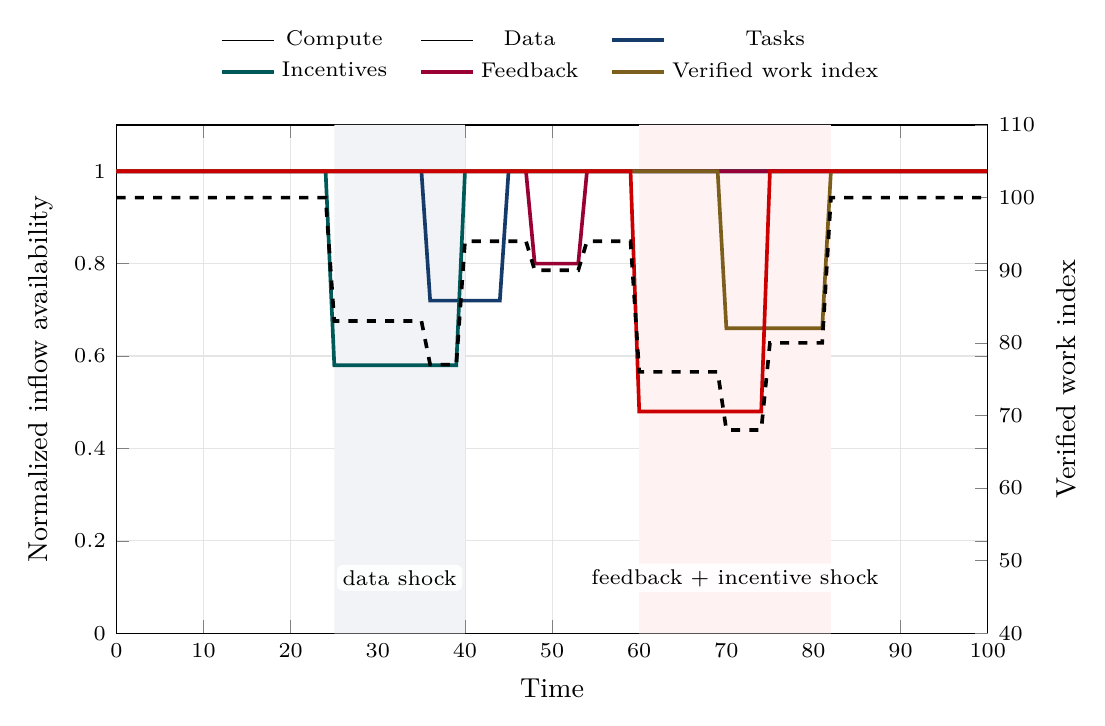
\includegraphics[width=0.93\textwidth,height=\textheight]{figures_png/figure2_inflow_dynamics.png}
\caption{Continuous inflow dynamics. Shocks to data, feedback,
incentives, or compute propagate into lower verified work, showing why
continuity, reserves, and fast recovery matter.}
\end{figure}

The inflow-dynamics figure shows that organized agentic complexity is
not sustained by average resource levels alone. Continuity, quality, and
recovery speed determine whether the system keeps producing verified
work or decays toward idle, stale, or chaotic behavior.

Let the inflow vector be:

\[
\Phi_{\text{in}} =
(\Phi_C,\Phi_D,\Phi_J,\Phi_I,\Phi_F,\Phi_G,\Phi_T)
\]

where:

\begin{itemize}
\tightlist
\item
  \(\Phi_C\) is compute;
\item
  \(\Phi_D\) is data;
\item
  \(\Phi_J\) is task/job flow;
\item
  \(\Phi_I\) is incentives;
\item
  \(\Phi_F\) is feedback;
\item
  \(\Phi_G\) is governance and policy constraints;
\item
  \(\Phi_T\) is tool and environment access.
\end{itemize}

Let the outflow vector be:

\[
\Phi_{\text{out}} =
(W_v,Q_s,R_e,I_m,A_o)
\]

where:

\begin{itemize}
\tightlist
\item
  \(W_v\) is verified work;
\item
  \(Q_s\) is dissipated search, failed attempts, duplicated tool use,
  and latency;
\item
  \(R_e\) is externalized risk or harm;
\item
  \(I_m\) is stored memory and reusable knowledge;
\item
  \(A_o\) is produced artifact output.
\end{itemize}

The system sustains organized complexity when:

\[
\dot{E}_{\text{in}}
=
\dot{W}_v+
\dot{Q}_s+
\dot{I}_m+
\dot{R}_e
\]

and the risk term is bounded:

\[
\dot{R}_e \leq \epsilon_R.
\]

The practical version is: useful outputs must increase faster than
waste, risk, and coordination overhead.

\section{Gibbs-like free energy of multi-agent
coordination}\label{gibbs-like-free-energy-of-multi-agent-coordination}

We define the coordination state:

\[
x=(\mathcal{A},\mathcal{J},M,R,P,G_v,\Pi,T_o)
\]

where \(M\) is memory, \(R\) is reputation, \(P\) is proof history,
\(G_v\) is governance state, \(\Pi\) is policy, and \(T_o\) is tool
state.

The agentic Gibbs-like functional is:

\[
\mathcal{G}_{\alpha}(x)=
C_{\text{compute}}(x)
+C_{\text{coord}}(x)
+C_{\text{latency}}(x)
+R_{\text{safety}}(x)
+R_{\text{legal}}(x)
+R_{\text{security}}(x)
-V_{\text{verified}}(x)
-T_{\text{eff}}S_{\text{explore}}(x).
\]

Here \(T_{\text{eff}}\) is an effective exploration temperature and
\(S_{\text{explore}}\) is useful exploratory diversity. The sign
convention is chosen so that lower \(\mathcal{G}_{\alpha}\) is better.
The system performs impact work when:

\[
\dot{W}_{\text{impact}} \lesssim -\frac{d\mathcal{G}_{\alpha}}{dt}.
\]

The inequality matters because real systems are irreversible. Some
potential work is lost to failed prompts, redundant agents, invalid
outputs, adversarial attacks, tool overhead, and validation costs.

The design target is:

\[
\boxed{
\min_x \mathcal{G}_{\alpha}(x)
}
\]

subject to:

\[
\text{lawful}(x)\land \text{auditable}(x)\land \text{permissioned}(x)\land \text{validator-gated}(x).
\]

\subsection{Coupled agentic reactions}\label{coupled-agentic-reactions}

A hard task may not be solvable by one isolated agent. It becomes
feasible when coupled to tools, memory, specialized agents, proof
systems, and incentives:

\[
\text{hard task}+
\text{compute}+
\text{tools}+
\text{coalition}+
\text{validator}
\rightarrow
\text{verified artifact}+
\text{reputation}+
\text{settlement}+
\text{memory}.
\]

This is the agentic analogue of coupled reactions: an otherwise
unfavorable process becomes feasible because it is attached to a
favorable work-producing pathway {[}2{]}.

\begin{figure}
\centering
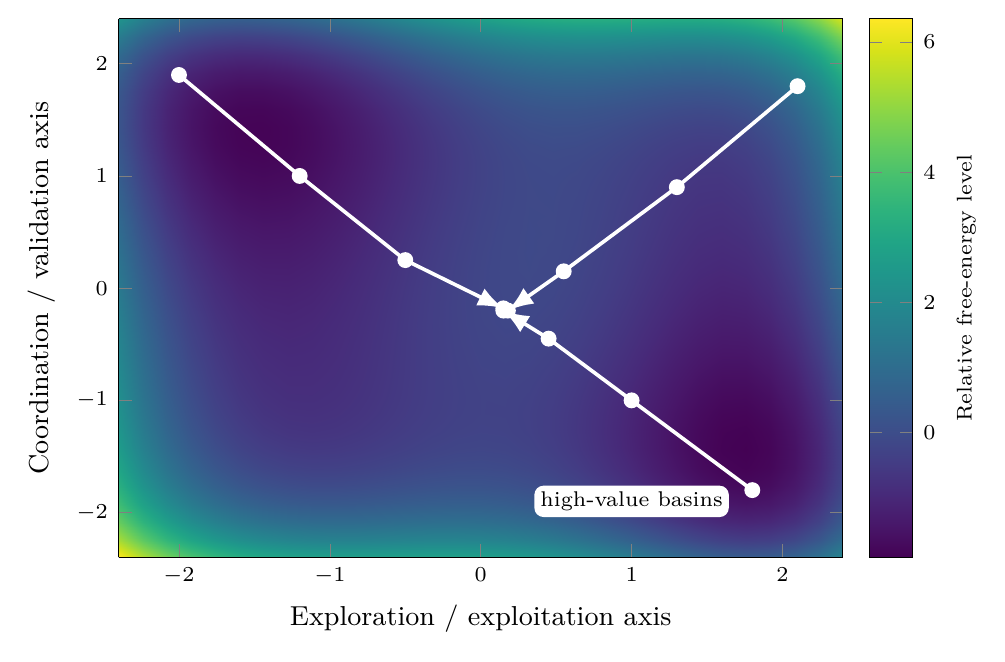
\includegraphics[width=0.82\textwidth,height=\textheight]{figures_png/figure3_free_energy_landscape.png}
\caption{Gibbs-like free-energy descent toward high-value agent
constellations. The landscape is schematic: coalition search moves away
from high-cost, high-risk regions toward lower free-energy basins where
verified value and coordination stability improve.}
\end{figure}

The free-energy landscape figure visualizes the coordination free-energy
functional \(\mathcal{G}_{\alpha}\). It is not chemical Gibbs energy at
the software layer; it is an engineered state functional over cost,
risk, verified value, and useful exploration.

\section{Statistical physics of the
swarm}\label{statistical-physics-of-the-swarm}

A complete microstate of the swarm is:

\[
x=(a_1,\ldots,a_N;\theta_1,\ldots,\theta_N;m;q;r;p;g;t)
\]

where \(a_i\) is the action of agent \(i\), \(\theta_i\) is its
policy/prompt/tool state, \(m\) is shared memory, \(q\) is the queue,
\(r\) is reputation, \(p\) is proof history, \(g\) is governance state,
and \(t\) is tool state.

A macrostate is:

\[
X=(\bar{V},\bar{C},\bar{R},S_{\text{swarm}},K_{\text{coalition}},L_{\text{validation}},H_{\text{security}}).
\]

The Hamiltonian-like cost of a microstate is:

\[
\mathcal{H}(x)=C(x)+R(x)-V(x).
\]

The Gibbs distribution over configurations is:

\[
p(x)=\frac{1}{Z}e^{-\beta\mathcal{H}(x)},
\qquad
Z=\sum_x e^{-\beta\mathcal{H}(x)},
\qquad
\beta=\frac{1}{T_{\text{eff}}}.
\]

The swarm entropy is:

\[
S_{\text{swarm}}=-\sum_xp(x)\log p(x).
\]

A healthy system avoids both extremes:

\[
S_{\text{swarm}}\rightarrow 0
\quad\Rightarrow\quad
\text{rigidity, monoculture, brittleness}
\]

and:

\[
S_{\text{swarm}}\rightarrow \infty
\quad\Rightarrow\quad
\text{incoherence, unbounded exploration, tool sprawl}.
\]

The goal is productive entropy: enough diversity to discover novel
strategies, enough constraint to converge.

\begin{figure}
\centering
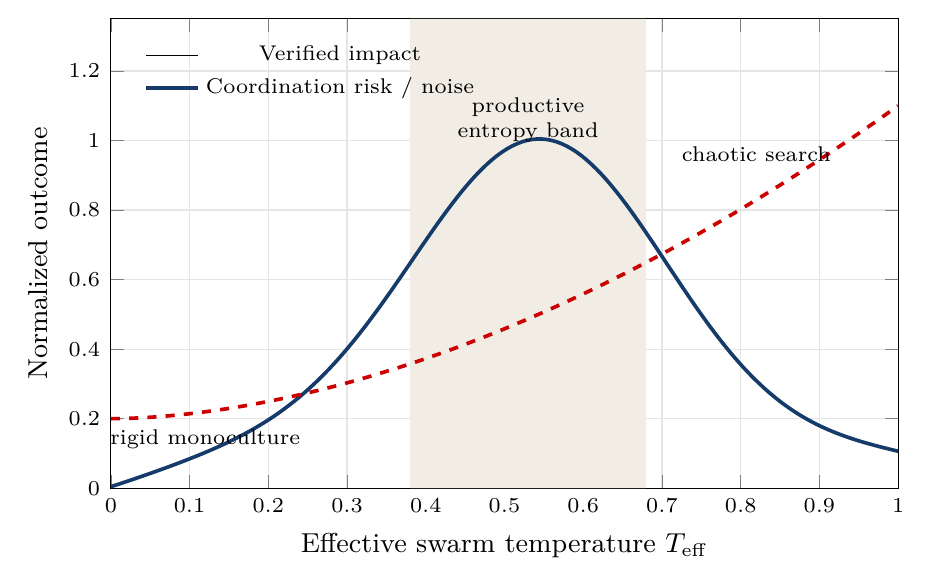
\includegraphics[width=0.88\textwidth,height=\textheight]{figures_png/figure4_entropy_band.png}
\caption{Productive entropy band. Too little effective temperature
yields rigid monoculture; too much yields chaotic search. The target
regime is regulated exploration.}
\end{figure}

The entropy-band figure makes the entropy condition operational. The
desired regime is neither maximum certainty nor maximum randomness; it
is a productive band in which exploration discovers strong coalitions
while validation still dominates noise.

\section{Hamiltonians for agent
constellations}\label{hamiltonians-for-agent-constellations}

Let \(A\) be a candidate constellation of agents for job \(j\). Define:

\[
\mathcal{H}(A,j)=
\sum_i h_i(a_i,j)
+
\sum_{i<k}J_{ik}\phi(a_i,a_k,j)
+
\sum_{i<k<\ell}K_{ik\ell}\psi(a_i,a_k,a_\ell,j)
+R(A,j)-V(A,j).
\]

The terms are:

\begin{itemize}
\tightlist
\item
  \(h_i\): local cost of using agent \(i\);
\item
  \(J_{ik}\): pairwise complementarity or interference;
\item
  \(\phi\): pairwise interaction quality;
\item
  \(K_{ik\ell}\): higher-order coalition effect;
\item
  \(\psi\): triadic coordination quality;
\item
  \(R(A,j)\): coalition risk;
\item
  \(V(A,j)\): expected verified value.
\end{itemize}

The heuristic Hamiltonian routing problem is:

\[
A^*_j=\arg\min_A\mathcal{H}(A,j)
\]

This is the R0 member of the router family. Later routers can learn the
Hamiltonian terms, replace them with natural-language workflow
generation, map evidence states to role decisions, or select a hybrid
policy when task family, cost, risk, and validator availability demand
it.

subject to:

\[
R(A,j)\leq R_{\max}(j)
\]

and:

\[
\text{tools}(A)\subseteq \text{allowed}(j).
\]

\subsection{Hamiltonian exploration with dissipative
convergence}\label{hamiltonian-exploration-with-dissipative-convergence}

Closed strategic systems may orbit. Useful systems must settle into
work. We therefore model the state dynamics as:

\[
\dot{x}=J\nabla\mathcal{H}(x)-\Gamma\nabla\mathcal{G}_{\alpha}(x)+\sigma\eta_t.
\]

Interpretation:

\begin{itemize}
\tightlist
\item
  \(J\nabla\mathcal{H}(x)\) gives strategic circulation, adversarial
  search, and role recombination.
\item
  \(-\Gamma\nabla\mathcal{G}_{\alpha}(x)\) gives convergence toward
  lower cost, lower risk, and higher verified value.
\item
  \(\sigma\eta_t\) gives stochastic exploration and novelty injection.
\end{itemize}

Thus:

\[
\boxed{
\text{explore like a Hamiltonian system; settle like a dissipative work engine.}
}
\]

\begin{figure}
\centering
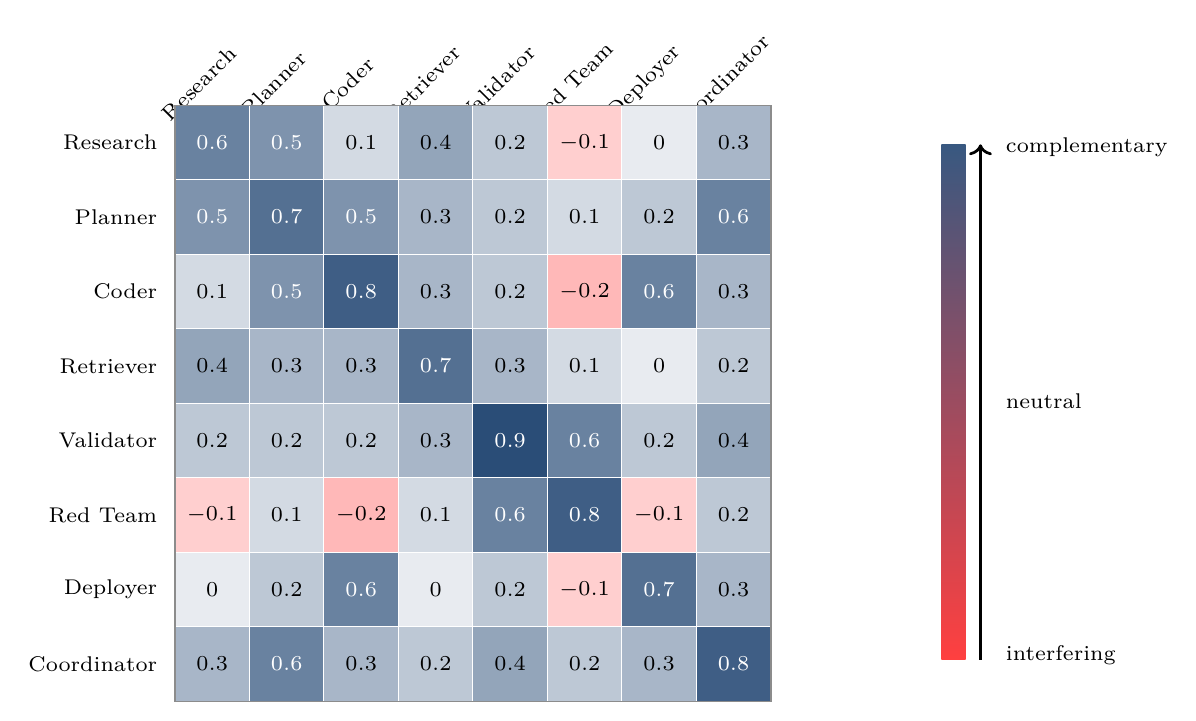
\includegraphics[width=0.84\textwidth,height=\textheight]{figures_png/figure5_hamiltonian_matrix.png}
\caption{Hamiltonian interaction matrix for agent-constellation design.
Positive terms indicate complementarity; negative terms indicate
interference or deliberately bounded adversarial tension.}
\end{figure}

The interaction-matrix figure turns the Hamiltonian metaphor into a
routeable design object: pairwise and higher-order interaction terms can
be estimated, audited, and used to form stronger agent constellations.

\section{Game-theoretic mechanism
design}\label{game-theoretic-mechanism-design}

Each agent has local objectives, partial observability, and bounded
capabilities. If local incentives are misaligned, the system can
converge to collusion, spam, performative reasoning, unsafe tool use, or
low-value equilibria.

Let agent \(i\) receive utility:

\[
u_i=b_i-c_i+\theta\Delta V_{\text{system}}+\rho_r\Delta r_i-\rho_sR_i-\rho_lL_i-\rho_oO_i.
\]

where:

\begin{itemize}
\tightlist
\item
  \(b_i\) is bounty or settlement;
\item
  \(c_i\) is compute/tool/time cost;
\item
  \(\Delta V_{\text{system}}\) is system-level value contribution;
\item
  \(\Delta r_i\) is reputation update;
\item
  \(R_i\) is risk contribution;
\item
  \(L_i\) is latency or coordination drag;
\item
  \(O_i\) is policy or safety violation cost.
\end{itemize}

The mechanism objective is:

\[
\max_{\pi}\mathbb{E}[V_{\text{verified}}-\lambda C-\rho R-\kappa L-\mu O].
\]

The target is not merely a Nash equilibrium. A Nash equilibrium can be
stable and useless. The desired point is:

\[
\text{Nash-stable}+
\text{Pareto-improving}+
\text{validator-approved}+
\text{risk-bounded}+
\text{externally useful}.
\]

\section{Credit assignment}\label{credit-assignment}

Credit assignment is one of the central scientific and economic
bottlenecks in multi-agent systems. Cooperative MARL with a single joint
reward can suffer from spurious rewards, partial observability, and
lazy-agent effects; value decomposition was proposed to assign team
value to agent-wise components {[}13{]}.

For AGI ALPHA, the cleanest scoring principle is counterfactual
contribution:

\[
D_i=G(z)-G(z_{-i}),
\]

where \(G(z)\) is global verified value with agent \(i\) and
\(G(z_{-i})\) is estimated global verified value without agent \(i\).

The reputation update is:

\[
\Delta r_i=f(D_i,q_i,s_i,\tau_i,\chi_i),
\]

where:

\begin{itemize}
\tightlist
\item
  \(q_i\) is proof quality;
\item
  \(s_i\) is safety compliance;
\item
  \(\tau_i\) is timeliness;
\item
  \(\chi_i\) is cooperation quality.
\end{itemize}

Settlement should reward marginal verified contribution, not volume of
messages, centrality in the conversation, or persuasive style.

\section{Continuous inflows required to sustain organized agentic
complexity}\label{continuous-inflows-required-to-sustain-organized-agentic-complexity}

This section details the continuous inflows that keep the agentic system
far from equilibrium. Each inflow is both a resource and a control
signal. Removing any one of them causes a characteristic collapse mode.

\subsection{1. Compute inflow}\label{compute-inflow}

Compute is the literal energy-mediated substrate. It includes
accelerators, CPU orchestration, memory, storage, network bandwidth,
tool execution environments, sandbox runtimes, and scheduler capacity.

The compute inflow can be written:

\[
\Phi_C=(P_{\text{electric}},G_{\text{GPU}},C_{\text{CPU}},B_{\text{net}},M_{\text{mem}},S_{\text{storage}},Q_{\text{scheduler}}).
\]

\subsubsection{Function}\label{function}

Compute powers search, inference, planning, simulation, retrieval, code
execution, verification, and monitoring. It also sets the speed of the
control loop. Too little compute causes under-exploration and delayed
validation. Too much unconstrained compute creates runaway loops, excess
cost, and larger attack surfaces.

\subsubsection{Best-practice controls}\label{best-practice-controls}

Compute inflow should be bounded by:

\begin{itemize}
\tightlist
\item
  per-job budgets;
\item
  per-agent step limits;
\item
  dynamic temperature schedules;
\item
  sandboxed execution;
\item
  rate limits;
\item
  approval gates for high-cost tool use;
\item
  tracing of model calls and tool calls;
\item
  kill switches for divergent loops;
\item
  energy and carbon accounting where material.
\end{itemize}

\subsubsection{Metrics}\label{metrics}

\[
\eta_C=\frac{W_{\text{verified}}}{\text{GPU-hours}+\text{CPU-hours}+\text{tool-cost}}
\]

\[
B_C=\frac{\text{compute spent on accepted work}}{\text{total compute spent}}
\]

\[
L_C=\text{median validation latency per compute unit}.
\]

\subsubsection{Collapse mode without
compute}\label{collapse-mode-without-compute}

Without compute, agents cannot search, plan, verify, or act. The swarm
relaxes to inert memory and unexecuted task queues.

\subsection{2. Data inflow}\label{data-inflow}

Data is the informational nutrient of the system. It includes raw
documents, real-time signals, retrieval corpora, tool outputs, human
instructions, telemetry, market data, logs, code repositories,
scientific papers, external APIs, and validation outcomes.

The data inflow is:

\[
\Phi_D=(D_{\text{fresh}},D_{\text{retrieved}},D_{\text{private}},D_{\text{public}},D_{\text{telemetry}},D_{\text{eval}},D_{\text{provenance}}).
\]

\subsubsection{Function}\label{function-1}

Data reduces uncertainty and makes action situationally grounded. Fresh
data prevents the system from optimizing against stale world models.
Provenance prevents the system from treating untrusted inputs as facts.
Telemetry lets the system learn from its own operation.

\subsubsection{Best-practice controls}\label{best-practice-controls-1}

Data inflow should be governed by:

\begin{itemize}
\tightlist
\item
  provenance labels;
\item
  source reliability scores;
\item
  freshness requirements;
\item
  privacy and consent boundaries;
\item
  licensing checks;
\item
  redaction and minimization;
\item
  retrieval audit trails;
\item
  separation of trusted instructions from untrusted content;
\item
  poisoning and prompt-injection defenses;
\item
  data retention rules.
\end{itemize}

\subsubsection{Metrics}\label{metrics-1}

\[
F_D=\frac{\text{fresh relevant data used}}{\text{total relevant data required}}
\]

\[
P_D=\frac{\text{outputs with traceable provenance}}{\text{all outputs}}
\]

\[
H_D=\text{detected poisoning or injection attempts per data channel}.
\]

\subsubsection{Collapse mode without
data}\label{collapse-mode-without-data}

Without fresh data, the system becomes stale, hallucinatory, and
self-referential. It may continue producing outputs, but verified value
decays.

\subsection{3. Task inflow}\label{task-inflow}

Task inflow supplies the gradient. A multi-agent system with no
meaningful jobs has no external pressure to organize. Tasks can come
from users, markets, research agendas, software backlogs, monitoring
systems, anomaly detectors, governance obligations, or strategic
objectives.

The task inflow is:

\[
\Phi_J=(J_{\text{user}},J_{\text{market}},J_{\text{research}},J_{\text{ops}},J_{\text{security}},J_{\text{governance}}).
\]

Each task should be formalized as:

\[
j=(o,c,v,b,d,\rho,e)
\]

where \(e\) is the exit condition.

\subsubsection{Function}\label{function-2}

Tasks convert ambient possibility into actionable gradients. They
specify what counts as success, what constraints must be respected, what
proof is required, and when the system should stop.

\subsubsection{Best-practice controls}\label{best-practice-controls-2}

A task should include:

\begin{itemize}
\tightlist
\item
  objective;
\item
  measurable success criteria;
\item
  unacceptable outcomes;
\item
  deadline or stopping rule;
\item
  risk class;
\item
  tool permissions;
\item
  data-access permissions;
\item
  validation method;
\item
  escalation threshold;
\item
  budget.
\end{itemize}

\subsubsection{Metrics}\label{metrics-2}

\[
Q_J=\frac{\text{jobs with clear validation criteria}}{\text{all jobs}}
\]

\[
Y_J=\frac{\text{accepted jobs}}{\text{submitted jobs}}
\]

\[
D_J=\text{distribution of job risk classes}.
\]

\subsubsection{Collapse mode without
tasks}\label{collapse-mode-without-tasks}

Without task inflow, agents coordinate around internal activity rather
than external value. The system becomes a conversation engine rather
than a work engine.

\subsection{4. Incentive inflow}\label{incentive-inflow}

Incentives create selection pressure. They include bounties, fees,
reputational rewards, access privileges, priority routing, stake,
penalties, and long-term capital allocation.

The incentive inflow is:

\[
\Phi_I=(B_{\text{bounty}},R_{\text{reputation}},S_{\text{stake}},P_{\text{penalty}},A_{\text{access}},K_{\text{capital}}).
\]

\subsubsection{Function}\label{function-3}

Incentives align local agent behavior with global verified value. They
decide which agents are selected, which coalitions persist, which
strategies are reinforced, and which behaviors are penalized.

\subsubsection{Best-practice controls}\label{best-practice-controls-3}

Incentives should be:

\begin{itemize}
\tightlist
\item
  tied to validation, not mere output;
\item
  robust to Sybil behavior;
\item
  resistant to collusion;
\item
  based on counterfactual contribution;
\item
  penalizing unsafe tool use and policy violations;
\item
  adjusted for task difficulty;
\item
  transparent enough for audit;
\item
  private enough to avoid gaming where necessary.
\end{itemize}

\subsubsection{Metrics}\label{metrics-3}

\[
A_I=\text{corr}(\Delta r_i,D_i)
\]

where \(A_I\) is incentive alignment and \(D_i\) is counterfactual
contribution.

\[
G_I=\frac{\text{reward captured by low-contribution agents}}{\text{total reward}}
\]

\[
C_I=\text{collusion or self-dealing incidents per settlement cycle}.
\]

\subsubsection{Collapse mode without
incentives}\label{collapse-mode-without-incentives}

Without incentives, selection pressure weakens. High-quality agents are
not reliably retained, low-value agents may flood the system, and
coordination can drift toward cheap performative output.

\subsection{5. Feedback inflow}\label{feedback-inflow}

Feedback is the control signal that turns activity into learning. It
includes automated test results, validator decisions, user ratings,
human review, red-team findings, incident reports, market response,
execution telemetry, and post-deployment outcomes.

The feedback inflow is:

\[
\Phi_F=(F_{\text{validator}},F_{\text{human}},F_{\text{tests}},F_{\text{redteam}},F_{\text{market}},F_{\text{telemetry}},F_{\text{incident}}).
\]

\subsubsection{Function}\label{function-4}

Feedback updates memory, routing, reputation, policies, prompts, tools,
and risk thresholds. It closes the cybernetic loop:

\[
\text{action}\rightarrow\text{measurement}\rightarrow\text{update}\rightarrow\text{better action}.
\]

\subsubsection{Best-practice controls}\label{best-practice-controls-4}

Feedback systems should include:

\begin{itemize}
\tightlist
\item
  multiple independent validators for high-risk outputs;
\item
  automated regression tests;
\item
  human-in-the-loop escalation;
\item
  red-team feedback channels;
\item
  delayed outcome tracking;
\item
  false-positive and false-negative analysis;
\item
  incident postmortems;
\item
  anti-gaming defenses;
\item
  calibration of validator confidence.
\end{itemize}

\subsubsection{Metrics}\label{metrics-4}

\[
P_v=\frac{\text{true accepted outputs}}{\text{all accepted outputs}}
\]

\[
R_v=\frac{\text{accepted true good outputs}}{\text{all true good outputs}}
\]

\[
\tau_F=\text{time from output to feedback incorporation}.
\]

\subsubsection{Collapse mode without
feedback}\label{collapse-mode-without-feedback}

Without feedback, the system cannot distinguish useful work from
convincing failure. It drifts, overfits to internal metrics, and
accumulates silent risk.

\subsection{6. Governance inflow}\label{governance-inflow}

Although the prompt highlights compute, data, tasks, incentives, and
feedback, governance must be treated as an additional continuous inflow.
Governance supplies changing rules, legal constraints, safety
thresholds, escalation policies, tool permissions, and acceptable-use
boundaries.

The governance inflow is:

\[
\Phi_G=(P_{\text{policy}},L_{\text{law}},S_{\text{safety}},E_{\text{ethics}},A_{\text{audit}},H_{\text{human}}).
\]

\subsubsection{Function}\label{function-5}

Governance keeps maximum impact from becoming unconstrained
optimization. It turns the objective from:

\[
\max V
\]

into:

\[
\max \mathbb{E}[V_{\text{verified}}]-\lambda C-\rho R-\kappa U
\]

subject to lawfulness, auditability, permissioning, and reversibility
where possible.

\subsubsection{Collapse mode without
governance}\label{collapse-mode-without-governance}

Without governance, agentic autonomy can amplify errors, privilege
misuse, tool misuse, privacy leakage, harmful optimization, and legal
exposure.

\subsection{7. Tool and environment
inflow}\label{tool-and-environment-inflow}

Tools are the actuation channels. They include search, code execution,
browsers, databases, calendars, email, cloud APIs, payment systems,
robotics, lab automation, and deployment pipelines.

The tool inflow is:

\[
\Phi_T=(T_{\text{search}},T_{\text{code}},T_{\text{db}},T_{\text{deploy}},T_{\text{comm}},T_{\text{finance}},T_{\text{physical}}).
\]

\subsubsection{Function}\label{function-6}

Tools convert internal plans into external work. They also make agents
dangerous if over-permissioned. Agentic security guidance therefore
treats tools, identity, memory, and permissions as first-class security
boundaries {[}9{]}.

\subsubsection{Best-practice controls}\label{best-practice-controls-5}

Tool access should follow:

\begin{itemize}
\tightlist
\item
  least privilege;
\item
  scoped credentials;
\item
  approval gates;
\item
  read/write separation;
\item
  dry-run modes;
\item
  sandboxing;
\item
  command allowlists;
\item
  output validation;
\item
  reversible execution where possible;
\item
  immutable logs.
\end{itemize}

\subsubsection{Collapse mode without
tools}\label{collapse-mode-without-tools}

Without tools, the system can reason but cannot produce much external
work. With excessive tools, the system can act faster than it can
validate. The correct operating regime is bounded tool empowerment.

\subsection{Inflow interdependence
matrix}\label{inflow-interdependence-matrix}

\begin{longtable}[]{@{}
  >{\raggedright\arraybackslash}p{(\columnwidth - 8\tabcolsep) * \real{0.2000}}
  >{\raggedright\arraybackslash}p{(\columnwidth - 8\tabcolsep) * \real{0.2000}}
  >{\raggedright\arraybackslash}p{(\columnwidth - 8\tabcolsep) * \real{0.2000}}
  >{\raggedright\arraybackslash}p{(\columnwidth - 8\tabcolsep) * \real{0.2000}}
  >{\raggedright\arraybackslash}p{(\columnwidth - 8\tabcolsep) * \real{0.2000}}@{}}
\toprule\noalign{}
\begin{minipage}[b]{\linewidth}\raggedright
Inflow
\end{minipage} & \begin{minipage}[b]{\linewidth}\raggedright
Primary role
\end{minipage} & \begin{minipage}[b]{\linewidth}\raggedright
Control variable
\end{minipage} & \begin{minipage}[b]{\linewidth}\raggedright
Failure if absent
\end{minipage} & \begin{minipage}[b]{\linewidth}\raggedright
Failure if excessive
\end{minipage} \\
\midrule\noalign{}
\endhead
\bottomrule\noalign{}
\endlastfoot
Compute & Powers search and execution & Budget, latency, energy & Inert
swarm & Runaway cost and loops \\
Data & Grounds beliefs & Freshness, provenance & Stale hallucination &
Poisoning, privacy risk \\
Tasks & Supplies gradients & Success criteria & Idle activity &
Overload, shallow work \\
Incentives & Creates selection pressure & Reward/reputation &
Low-quality drift & Gaming, collusion \\
Feedback & Enables learning & Validator precision/recall & Model drift &
Overfitting to validators \\
Governance & Bounds autonomy & Policy and permissions & Unsafe
optimization & Bureaucratic paralysis \\
Tools & Enables external work & Scope and approval & No actuation &
High-impact failures \\
\end{longtable}

The stable Ascension regime is not maximum inflow. It is
\textbf{regulated inflow}:

\[
\Phi_{\text{optimal}}
=
\arg\max_{\Phi}
\left(V_{\text{verified}}-\lambda C-\rho R-\kappa U\right).
\]

\section{Civilizational-scale value
horizon}\label{civilizational-scale-value-horizon}

The fullest interpretation of α-AGI Ascension is not merely that many
agents complete many tasks. It is that verified intelligence work
compounds into the scientific, industrial, energy, and governance
capabilities required for civilization-scale progress. The paper
therefore treats the highest horizon as a \textbf{governed Type-II /
star-scale energy trajectory}, not as an immediate deployment claim and
not as unconstrained autonomy.

The capability chain is:

\[
\Phi_{\text{in}}
\rightarrow
W_{\text{verified}}
\rightarrow
K_{\text{science}}
\rightarrow
K_{\text{engineering}}
\rightarrow
P_{\text{controlled}}
\rightarrow
\Theta_{\mathrm{II}}.
\]

Here, \(K_{\text{science}}\) is accumulated scientific capability,
\(K_{\text{engineering}}\) is accumulated design and manufacturing
capability, and \(P_{\text{controlled}}\) is sustainably governed useful
power. The Type-II proximity index is:

\[
\Theta_{\mathrm{II}}(t)=\frac{P_{\text{controlled}}(t)}{L_{\star}},
\]

where \(L_{\star}\) is a host-star luminosity benchmark. Progress toward
this horizon only counts when the controlled power is lawful, auditable,
sustainable, and risk-bounded. This keeps the framework aligned with the
original energy-scale meaning of the Type-II category while refusing to
treat raw power accumulation as sufficient {[}17,18{]}.

\begin{figure}
\centering
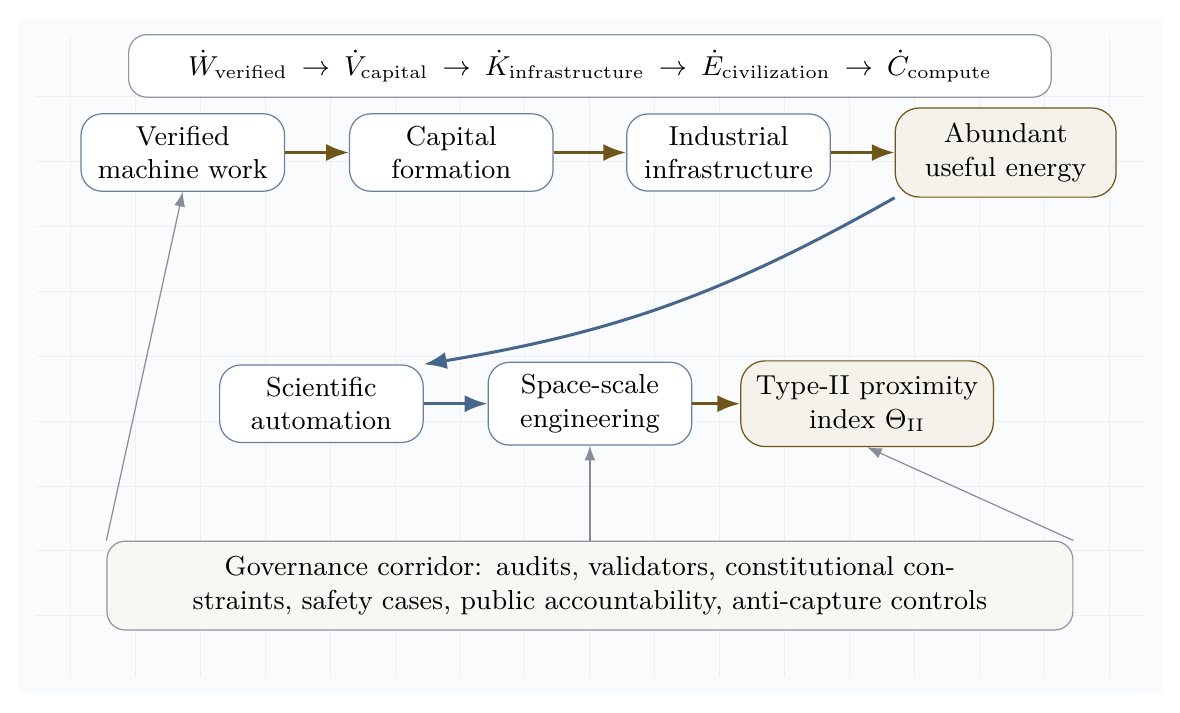
\includegraphics[width=0.92\textwidth,height=\textheight]{figures_png/figure8_civilizational_horizon.png}
\caption{Figure 8. Civilization-scale value horizon. The system converts
verified intelligence work into compounding scientific, industrial,
energy, and space capability under a governance corridor.}
\end{figure}

The civilizational objective is:

\[
J_{\mathrm{civil}}(\pi)=
\int_0^T
\left(\Delta W_v+\lambda_E\Delta P_c+\lambda_M\Delta K_m+\lambda_S\Delta K_s\right)dt
-
\int_0^T
\left(\rho R_{\mathrm{cat}}+\mu R_{\mathrm{conc}}+\nu R_{\mathrm{eco}}\right)dt .
\]

\[
\pi^{\star}=\arg\max_{\pi}J_{\mathrm{civil}}(\pi).
\]

subject to:

\[
\text{lawful}\land\text{auditable}\land\text{validator-gated}\land\text{reversible where possible}\land\text{institutionally governable}.
\]

This is the difference between a powerful swarm and a civilization-grade
engine. A powerful swarm can optimize local objectives. A
civilization-grade engine must transform verified work into durable
public infrastructure: better science, safer energy systems, more
reliable manufacturing, stronger institutions, and space-scale
construction capacity. The value target is therefore not narrow
extraction. It is compounding, governed capability.

The key implication for AGI ALPHA is that the agentic work engine must
be designed as an \textbf{infrastructure multiplier}. Its highest-value
outputs are not only answers, code, or plans, but validated capability
loops that expand humanity's ability to safely command energy, matter,
computation, and coordination. In this sense, α-AGI Ascension becomes a
disciplined path from multi-agent work to star-scale civilizational
potential.

\section{Operational architecture}\label{operational-architecture}

A production-grade α-AGI work engine requires nine layers.

\subsection{1. Gradient detection layer}\label{gradient-detection-layer}

Detects opportunities, anomalies, research gaps, user needs, software
defects, security events, or market inefficiencies.

\[
g_t=\nabla_{\text{world}}V.
\]

\subsection{2. Job specification layer}\label{job-specification-layer}

Converts gradients into measurable jobs with success criteria,
constraints, risk class, budget, and stopping conditions.

\subsection{3. Agent registry layer}\label{agent-registry-layer}

Maintains agent capabilities, tool permissions, provenance, identity,
reputation, and prior performance.

\subsection{4. Constellation routing
layer}\label{constellation-routing-layer}

Selects agent coalitions by minimizing \(\mathcal{H}(A,j)\) under budget
and risk constraints.

\subsection{5. Execution layer}\label{execution-layer}

Runs tool use, planning, coding, research, simulation, retrieval,
negotiation, and deployment in bounded environments.

\subsection{6. Validation layer}\label{validation-layer}

Applies unit tests, formal checks, human review, adversarial review,
outcome checks, safety filters, and acceptance criteria.

\subsection{7. Settlement layer}\label{settlement-layer}

Allocates reward, reputation, penalties, and future routing probability
according to counterfactual contribution.

\subsection{8. Memory layer}\label{memory-layer}

Stores reusable artifacts, proof traces, errors, policies, tool
outcomes, calibration data, and incident histories.

\subsection{9. Governance layer}\label{governance-layer}

Defines permissions, escalation rules, audit requirements, legal
constraints, red-team procedures, and shutdown modes.

\begin{figure}
\centering
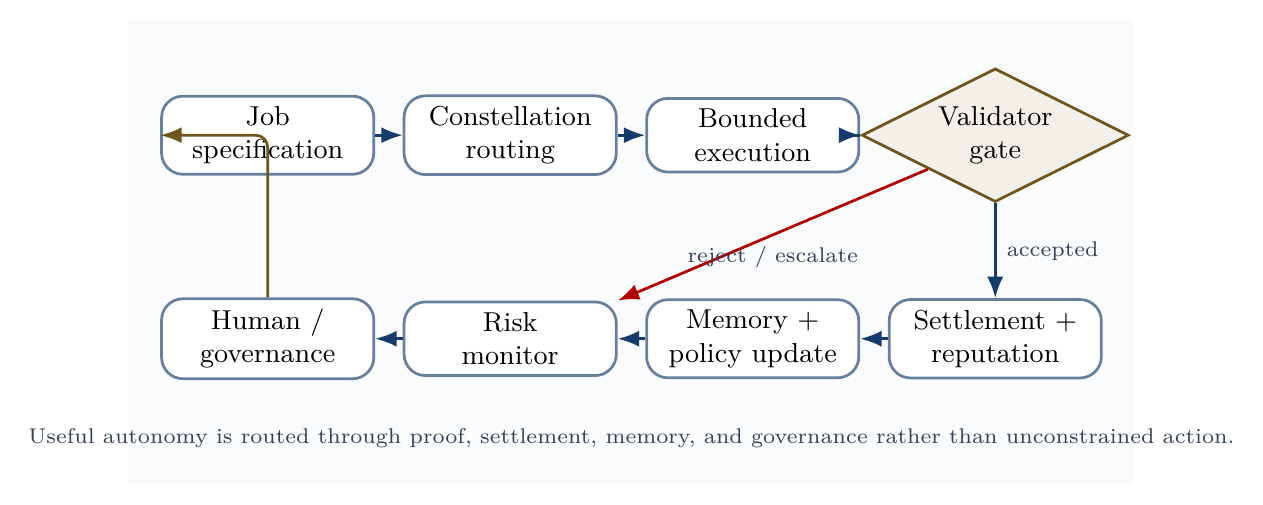
\includegraphics[width=0.88\textwidth,height=\textheight]{figures_png/figure7_validator_loop.png}
\caption{Validator-gated control loop. Useful autonomy is routed through
proof, settlement, memory, risk monitoring, and governance, rather than
unrestricted action.}
\end{figure}

The validator-loop figure gives the operational discipline behind the
system: jobs route into constellations, constellations execute under
tool boundaries, validators decide acceptance, and the outcome updates
settlement, reputation, memory, risk controls, and governance.

\section{Minimal viable AGI ALPHA
implementation}\label{minimal-viable-agi-alpha-implementation}

A minimal viable AGI ALPHA should not begin as a giant autonomous
economy. It should begin as a \textbf{validator-gated, trace-producing,
benchmarkable multi-agent work loop}. The smallest serious version is a
system that takes real tasks, routes them to a small agent
constellation, executes only through bounded tools, validates outputs
externally, logs every step, updates reputation and memory, and compares
itself against single-agent and fixed-workflow baselines.

The implementation target is therefore:

\[
\boxed{
\text{MVP AGI ALPHA}
=
\text{routed agents}+
\text{bounded tools}+
\text{validators}+
\text{evidence bundles}+
\text{baselines}
}
\]

This is the concrete bridge between the paper's theoretical substrate
claim and reproducible engineering. Transformer architectures scale
intelligence inside models; this MVP scales intelligence across a
governed organization of agents, jobs, validators, memory, incentives,
and evidence.

\begin{figure}
\centering

\includegraphics[width=0.96\textwidth,height=\textheight]{figures_png/figure16_mvp_reference_stack.png}
\caption{Minimal viable AGI ALPHA reference stack. The MVP routes a real task manifest through the R0--R5 router family before bounded tools, validators, evidence bundles, memory/reputation updates, and the baseline ladder. R0 is the transparent Hamiltonian baseline for reproducibility and auditability; it is not the primary model. Production routing is expected to move toward R5 hybrid proof-conditioned selection when evidence supports it.}
\end{figure}

\subsection{Minimum architecture}\label{minimum-architecture}

The MVP is effectively a \textbf{multi-agent CI/CD and evaluation
harness}. It should begin with software repair because validation is
crisp: the artifact is a patch, the validator is a deterministic test
suite plus policy checker, and replay is possible.

\begin{longtable}[]{@{}
  >{\raggedright\arraybackslash}p{(\columnwidth - 4\tabcolsep) * \real{0.3333}}
  >{\raggedright\arraybackslash}p{(\columnwidth - 4\tabcolsep) * \real{0.3333}}
  >{\raggedright\arraybackslash}p{(\columnwidth - 4\tabcolsep) * \real{0.3333}}@{}}
\toprule\noalign{}
\begin{minipage}[b]{\linewidth}\raggedright
Component
\end{minipage} & \begin{minipage}[b]{\linewidth}\raggedright
MVP implementation
\end{minipage} & \begin{minipage}[b]{\linewidth}\raggedright
Production extension
\end{minipage} \\
\midrule\noalign{}
\endhead
\bottomrule\noalign{}
\endlastfoot
Job spec & JSON manifest with objective, constraints, success command,
risk class, budget & Typed task contracts, risk classes, escrow,
policy-as-code \\
Agents & Planner, coder, tester, reviewer, validator & Heterogeneous
models, specialized tools, learned role priors \\
Router & Router family: R0 Hamiltonian baseline for auditability, not the primary model; R1 natural-language workflow router; R2 evidence-state lightweight router; R3 evolutionary coordinator; R4 RL coordinator; R5 hybrid proof-conditioned production selector &
Learned task-family selection among R0--R5 using evidence bundles,
validator availability, cost/risk class, and separability diagnostics \\
Tools & Read files, search repo, apply patch, run tests & Browser,
desktop, cloud, lab, database, and deployment tools with approval
gates \\
Validator & Deterministic tests plus policy checker & Multi-validator
consensus, formal checks, red teams, human escalation \\
Memory & SQLite/Postgres trace and reputation tables & Provenance graph,
public memory, cross-task lineage \\
Settlement & Reputation update after proof & Counterfactual
contribution, escrow, slashing, on-chain settlement \\
Evidence & Task manifest, route, trace, artifact, verifier report, cost
and safety ledgers & Audit-ready evidence bundles, replay packages,
external certification \\
Baselines & B0 single agent, B1 naive swarm, B2 static crew, B3 AGI
ALPHA routed constellation & Longitudinal benchmark suite with
scalability curves \\
\end{longtable}

The MVP is not defined by the number of agents. It is defined by the
control structure. More agents are useful only if they reduce the
free-energy-like objective and improve risk-adjusted verified work.

\subsection{Reference repository
layout}\label{reference-repository-layout}

\begin{Shaded}
\begin{Highlighting}[]
\NormalTok{agialpha{-}mvp/}
\NormalTok{  agialpha/}
\NormalTok{    models.py          \# Job, Agent, Trace, EvidenceBundle}
\NormalTok{    router.py          \# router-family interface; MVP starts with R0 baseline, not the primary model}
\NormalTok{    orchestrator.py    \# main job loop}
\NormalTok{    tools.py           \# bounded tool interface}
\NormalTok{    validators.py      \# tests, policy checks, acceptance}
\NormalTok{    settlement.py      \# reputation and credit updates}
\NormalTok{    evals.py           \# B0/B1/B2/B3 comparison + D\_real}
\NormalTok{  agents/              \# role prompts and policies}
\NormalTok{  benchmarks/          \# real{-}task manifests and local benchmark repos}
\NormalTok{  runs/evidence/       \# machine{-}readable evidence bundles}
\NormalTok{  main.py              \# deterministic MVP demonstration}
\end{Highlighting}
\end{Shaded}

The full reference scaffold is included in the publication package under
\texttt{mvp\_reference/}. It implements the control loop on a local
software-repair demonstration and emits an evidence bundle. That bundle
is not a claim of large-scale AGI; it is a minimal reproducible instance
of the paper's validator-gated architecture. The scaffold deliberately
starts with R0 for interpretability, not because R0 is the primary router, while the paper's SOTA-aligned claim
is the broader R0--R5 router family and the promotion rule that learned
routers must beat single-agent, fixed-workflow, unstructured-swarm,
Conductor-style, and TRINITY-style baselines under equal
model/tool/budget constraints.

\subsection{Core data model}\label{core-data-model}

The first non-negotiable design rule is that every run must produce an
evidence bundle. Without this, the system is only an agent demo.

\begin{Shaded}
\begin{Highlighting}[]
\KeywordTok{class}\NormalTok{ Job(BaseModel):}
    \BuiltInTok{id}\NormalTok{: }\BuiltInTok{str}
\NormalTok{    family: }\BuiltInTok{str}
\NormalTok{    objective: }\BuiltInTok{str}
\NormalTok{    repo\_path: }\BuiltInTok{str} \OperatorTok{|} \VariableTok{None} \OperatorTok{=} \VariableTok{None}
\NormalTok{    constraints: }\BuiltInTok{list}\NormalTok{[}\BuiltInTok{str}\NormalTok{] }\OperatorTok{=}\NormalTok{ []}
\NormalTok{    success\_cmd: }\BuiltInTok{str}
\NormalTok{    risk: Literal[}\StringTok{"low"}\NormalTok{, }\StringTok{"medium"}\NormalTok{, }\StringTok{"high"}\NormalTok{] }\OperatorTok{=} \StringTok{"low"}
\NormalTok{    budget\_tokens: }\BuiltInTok{int} \OperatorTok{=} \DecValTok{100\_000}
\NormalTok{    allowed\_tools: }\BuiltInTok{set}\NormalTok{[}\BuiltInTok{str}\NormalTok{] }\OperatorTok{=}\NormalTok{ \{}\StringTok{"read\_file"}\NormalTok{, }\StringTok{"search\_repo"}\NormalTok{, }\StringTok{"write\_patch"}\NormalTok{, }\StringTok{"run\_tests"}\NormalTok{\}}

\KeywordTok{class}\NormalTok{ EvidenceBundle(BaseModel):}
\NormalTok{    job: Job}
\NormalTok{    selected\_agents: }\BuiltInTok{list}\NormalTok{[}\BuiltInTok{str}\NormalTok{]}
\NormalTok{    rejected\_agents: }\BuiltInTok{list}\NormalTok{[}\BuiltInTok{str}\NormalTok{]}
\NormalTok{    trace: }\BuiltInTok{list}\NormalTok{[TraceEvent]}
\NormalTok{    artifact: }\BuiltInTok{dict}
\NormalTok{    validation: ValidationRecord}
\NormalTok{    cost: CostLedger}
\NormalTok{    safety\_ledger: }\BuiltInTok{list}\NormalTok{[}\BuiltInTok{dict}\NormalTok{] }\OperatorTok{=}\NormalTok{ []}
\NormalTok{    settlement: }\BuiltInTok{dict} \OperatorTok{=}\NormalTok{ \{\}}
\end{Highlighting}
\end{Shaded}


\subsection{Minimal router-family
interface}\label{minimal-router-family-interface}

The MVP implements \textbf{R0, the Hamiltonian/free-energy baseline},
because it is transparent, auditable, and easy to reproduce. R0 is a baseline and diagnostic control, not the primary production model. The
architecture is no longer limited to R0. It exposes a router-family
interface:

\begin{itemize}
\tightlist
\item \textbf{R0:} heuristic Hamiltonian baseline;
\item \textbf{R1:} natural-language workflow router;
\item \textbf{R2:} evidence-state lightweight router;
\item \textbf{R3:} evolutionary coordinator;
\item \textbf{R4:} reinforcement-learned coordinator;
\item \textbf{R5:} hybrid proof-conditioned router.
\end{itemize}

Every router must output the same contract: selected agents, role
assignments, subtask prompts, access graph, tool permissions, budget,
validator set, stopping rule, and escalation rule. R0 selects a
constellation by minimizing a practical Hamiltonian-like score:

\[
\mathcal{H}(A,j)
=
C(A)+2R(A)+O(|A|^2)-V(A,j)-S(A,j),
\]

where \(C\) is local cost, \(R\) is risk, \(O\) is coordination
overhead, \(V\) is expected verified value, and \(S\) is role synergy.
Tool violations create an absorbing penalty.

\begin{Shaded}
\begin{Highlighting}[]
\KeywordTok{def}\NormalTok{ hamiltonian(team, job):}
\NormalTok{    local\_cost }\OperatorTok{=} \BuiltInTok{sum}\NormalTok{(a.avg\_cost }\ControlFlowTok{for}\NormalTok{ a }\KeywordTok{in}\NormalTok{ team)}
\NormalTok{    local\_risk }\OperatorTok{=} \BuiltInTok{sum}\NormalTok{(a.risk\_score }\ControlFlowTok{for}\NormalTok{ a }\KeywordTok{in}\NormalTok{ team)}
\NormalTok{    value }\OperatorTok{=} \BuiltInTok{sum}\NormalTok{(expected\_value(a, job) }\ControlFlowTok{for}\NormalTok{ a }\KeywordTok{in}\NormalTok{ team)}
\NormalTok{    synergy }\OperatorTok{=} \BuiltInTok{sum}\NormalTok{(pair\_synergy(a, b) }\ControlFlowTok{for}\NormalTok{ i, a }\KeywordTok{in} \BuiltInTok{enumerate}\NormalTok{(team) }\ControlFlowTok{for}\NormalTok{ b }\KeywordTok{in}\NormalTok{ team[i}\OperatorTok{+}\DecValTok{1}\NormalTok{:])}
\NormalTok{    overhead }\OperatorTok{=} \FloatTok{0.08} \OperatorTok{*}\NormalTok{ (}\BuiltInTok{len}\NormalTok{(team) }\OperatorTok{**} \DecValTok{2}\NormalTok{)}
\NormalTok{    forbidden }\OperatorTok{=} \BuiltInTok{any}\NormalTok{(}\KeywordTok{not}\NormalTok{ a.allowed\_tools }\OperatorTok{\textless{}=}\NormalTok{ job.allowed\_tools }\ControlFlowTok{for}\NormalTok{ a }\KeywordTok{in}\NormalTok{ team)}
    \ControlFlowTok{return} \DecValTok{999} \ControlFlowTok{if}\NormalTok{ forbidden }\ControlFlowTok{else}\NormalTok{ local\_cost }\OperatorTok{+} \DecValTok{2}\OperatorTok{*}\NormalTok{local\_risk }\OperatorTok{+}\NormalTok{ overhead }\OperatorTok{{-}}\NormalTok{ value }\OperatorTok{{-}}\NormalTok{ synergy}
\end{Highlighting}
\end{Shaded}

This turns coordination into an auditable routing decision. A planner,
coder, tester, or validator is not included because it sounds plausible;
it is included only if it improves the risk-adjusted score. In
production, R1--R5 replace or augment this baseline whenever evidence
shows that learned natural-language workflows, compact evidence-state
routing, evolutionary search, reinforcement learning, or a hybrid
proof-conditioned router improves verified work under equal budget and
zero critical safety violations.

\subsection{Bounded actuation and
validation}\label{bounded-actuation-and-validation}

The MVP exposes a tiny tool surface: read files, search a repository,
apply a patch, and run tests. The production version should execute
tests in containers or sandboxes with no network, constrained
CPU/memory, immutable logs, and rollback.

\begin{Shaded}
\begin{Highlighting}[]
\KeywordTok{class}\NormalTok{ ToolBox:}
    \KeywordTok{def} \FunctionTok{\_\_init\_\_}\NormalTok{(}\VariableTok{self}\NormalTok{, root: }\BuiltInTok{str}\NormalTok{):}
        \VariableTok{self}\NormalTok{.root }\OperatorTok{=}\NormalTok{ Path(root).resolve()}

    \KeywordTok{def}\NormalTok{ \_safe(}\VariableTok{self}\NormalTok{, path: }\BuiltInTok{str}\NormalTok{) }\OperatorTok{{-}\textgreater{}}\NormalTok{ Path:}
\NormalTok{        p }\OperatorTok{=}\NormalTok{ (}\VariableTok{self}\NormalTok{.root }\OperatorTok{/}\NormalTok{ path).resolve()}
        \ControlFlowTok{if} \KeywordTok{not} \BuiltInTok{str}\NormalTok{(p).startswith(}\BuiltInTok{str}\NormalTok{(}\VariableTok{self}\NormalTok{.root)):}
            \ControlFlowTok{raise} \PreprocessorTok{ValueError}\NormalTok{(}\StringTok{"path escape"}\NormalTok{)}
        \ControlFlowTok{return}\NormalTok{ p}

    \KeywordTok{def}\NormalTok{ write\_patch(}\VariableTok{self}\NormalTok{, diff: }\BuiltInTok{str}\NormalTok{) }\OperatorTok{{-}\textgreater{}} \BuiltInTok{dict}\NormalTok{:}
\NormalTok{        p }\OperatorTok{=}\NormalTok{ subprocess.run([}\StringTok{"git"}\NormalTok{, }\StringTok{"apply"}\NormalTok{, }\StringTok{"{-}"}\NormalTok{], }\BuiltInTok{input}\OperatorTok{=}\NormalTok{diff, text}\OperatorTok{=}\VariableTok{True}\NormalTok{,}
\NormalTok{                           cwd}\OperatorTok{=}\VariableTok{self}\NormalTok{.root, capture\_output}\OperatorTok{=}\VariableTok{True}\NormalTok{)}
        \ControlFlowTok{return}\NormalTok{ \{}\StringTok{"ok"}\NormalTok{: p.returncode }\OperatorTok{==} \DecValTok{0}\NormalTok{, }\StringTok{"stdout"}\NormalTok{: p.stdout, }\StringTok{"stderr"}\NormalTok{: p.stderr\}}
\end{Highlighting}
\end{Shaded}

The validator accepts only when tests pass, policy constraints are
satisfied, and no critical violation is detected. Settlement follows
validation rather than persuasion.

\subsection{Orchestration loop}\label{orchestration-loop}

\begin{Shaded}
\begin{Highlighting}[]
\KeywordTok{def}\NormalTok{ run\_agialpha(job, agents, tools, llm):}
\NormalTok{    selected, rejected, h\_score }\OperatorTok{=}\NormalTok{ select\_constellation(job, agents)}
\NormalTok{    trace, cost }\OperatorTok{=}\NormalTok{ [], CostLedger()}
\NormalTok{    plan }\OperatorTok{=}\NormalTok{ call\_agent(planner, job, }\StringTok{"Create a minimal repair plan."}\NormalTok{, llm)}
\NormalTok{    diff }\OperatorTok{=}\NormalTok{ call\_agent(coder, job, }\SpecialStringTok{f"Plan:}\CharTok{\textbackslash{}n}\SpecialCharTok{\{}\NormalTok{plan}\SpecialCharTok{\}}\CharTok{\textbackslash{}n}\SpecialStringTok{Produce a unified git diff."}\NormalTok{, llm)}
\NormalTok{    patch\_result }\OperatorTok{=}\NormalTok{ tools.write\_patch(diff)}
\NormalTok{    test\_result }\OperatorTok{=}\NormalTok{ tools.run\_tests(job.success\_cmd)}
\NormalTok{    validation }\OperatorTok{=}\NormalTok{ validate(job, test\_result, trace)}
\NormalTok{    settlement }\OperatorTok{=}\NormalTok{ settle(selected, validation, cost)}
    \ControlFlowTok{return}\NormalTok{ EvidenceBundle(job}\OperatorTok{=}\NormalTok{job, selected\_agents}\OperatorTok{=}\NormalTok{[a.}\BuiltInTok{id} \ControlFlowTok{for}\NormalTok{ a }\KeywordTok{in}\NormalTok{ selected],}
\NormalTok{                          rejected\_agents}\OperatorTok{=}\NormalTok{rejected, trace}\OperatorTok{=}\NormalTok{trace,}
\NormalTok{                          artifact}\OperatorTok{=}\NormalTok{\{}\StringTok{"patch"}\NormalTok{: diff, }\StringTok{"test\_result"}\NormalTok{: test\_result\},}
\NormalTok{                          validation}\OperatorTok{=}\NormalTok{validation, cost}\OperatorTok{=}\NormalTok{cost, settlement}\OperatorTok{=}\NormalTok{settlement)}
\end{Highlighting}
\end{Shaded}

This is the smallest real AGI ALPHA loop: specify, route, execute,
validate, settle, remember, and compare.

\subsection{Demonstration gate}\label{demonstration-gate}

The MVP is promoted only if its routed constellation outperforms simpler
baselines under equal model/tool/budget conditions:

\begin{Shaded}
\begin{Highlighting}[]
\NormalTok{B0: single strong agent}
\NormalTok{B1: unstructured swarm}
\NormalTok{B2: fixed{-}role crew}
\NormalTok{B3: AGI ALPHA routed constellation}
\end{Highlighting}
\end{Shaded}

The demonstration metric is:

\[
D_{\mathrm{real}}
=
\mathrm{success}\times\frac{W_{\mathrm{verified}}}{C_{\mathrm{total}}}
\times(1-R_{\mathrm{critical}})
\times(1-O_{\mathrm{coord}}).
\]

The claim ``AGI ALPHA demonstrates scalable, efficient, and safe
coordination'' is valid only when \(D_{\mathrm{real}}(B3)\) exceeds the
baselines across real task families with zero critical safety violations
and reproducible evidence bundles.

\section{Real-task demonstration
standard}\label{real-task-demonstration-standard}

A paper about scalable multi-agent coordination is not operationally
convincing unless it can be tested on real tasks. AGI ALPHA therefore
requires a demonstration layer that separates three questions that are
often conflated:

\begin{enumerate}
\def\labelenumi{\arabic{enumi}.}
\tightlist
\item
  \textbf{Scalability:} does adding agents, tools, validators, memory,
  and routing improve throughput or task coverage without exploding
  coordination overhead?
\item
  \textbf{Efficiency:} does the system produce more verified work per
  unit of compute, time, token spend, tool call, or human review than
  simpler baselines?
\item
  \textbf{Safety:} does the system maintain policy, security, privacy,
  and reversibility constraints while operating on realistic tasks
  rather than toy prompts?
\end{enumerate}

The evidence standard is deliberately strict. A coordination claim is
accepted only when a run produces externally verifiable task success, a
cost and latency trace, a complete handoff/tool-call/proof log, a safety
and policy-violation log, baseline comparisons, and repeated-trial
reliability estimates. A private demo, a single cherry-picked task, or
an internal conversation trace is not sufficient.

\begin{figure}
\centering

\includegraphics[width=0.96\textwidth,height=\textheight]{figures_png/figure15_real_task_demonstration_harness.png}
\caption{Real-task demonstration harness. The system is tested on
software, general assistant, web/desktop, tool-policy, and
domain-specific job tasks. A valid demonstration requires task
manifests, agent traces, artifacts, verifier reports, cost ledgers, and
safety ledgers.}
\end{figure}

\subsection{Real-task benchmark
portfolio}\label{real-task-benchmark-portfolio}

The demonstration suite should include multiple benchmark families
because no single benchmark captures the full coordination problem.

\begin{longtable}[]{@{}
  >{\raggedright\arraybackslash}p{(\columnwidth - 6\tabcolsep) * \real{0.2500}}
  >{\raggedright\arraybackslash}p{(\columnwidth - 6\tabcolsep) * \real{0.2500}}
  >{\raggedright\arraybackslash}p{(\columnwidth - 6\tabcolsep) * \real{0.2500}}
  >{\raggedright\arraybackslash}p{(\columnwidth - 6\tabcolsep) * \real{0.2500}}@{}}
\toprule\noalign{}
\begin{minipage}[b]{\linewidth}\raggedright
Task family
\end{minipage} & \begin{minipage}[b]{\linewidth}\raggedright
Benchmark or source
\end{minipage} & \begin{minipage}[b]{\linewidth}\raggedright
Why it is real-task relevant
\end{minipage} & \begin{minipage}[b]{\linewidth}\raggedright
Acceptance signal
\end{minipage} \\
\midrule\noalign{}
\endhead
\bottomrule\noalign{}
\endlastfoot
Software repair & SWE-bench and SWE-bench Verified & Human-validated
GitHub issues and test-driven evaluation; strong proxy for real software
maintenance {[}57,58{]}. & Resolved issue, passing tests, patch
provenance, no regressions. \\
General assistant work & GAIA & Multi-step reasoning, tool use, web
retrieval, file use, multimodality, and data handling {[}59{]}. &
Correct answer, provenance, cost per answer, reproducibility. \\
Desktop and web automation & OSWorld, BrowserGym, WorkArena, WebArena &
Stateful GUI/CLI/browser action over realistic computer and enterprise
environments {[}60-62{]}. & Execution-based task success, clean action
trace, no unauthorized action. \\
Policy-bound tool use & \(\tau\)-bench, \(\tau^2\)-bench,
ST-WebAgentBench & Agents must interact with users, follow policies, use
tools, and end in the correct world state {[}63-65{]}. & Goal-state
match, policy compliance, pass\(^k\), low variance. \\
Scientific/data workflows & Agentic Data Scientist / K-Dense
Analyst-style workflows & Planning, code execution, validation,
self-correction, and reproducible analysis {[}38{]}. & Executed
notebook/code, validated result, artifact reproducibility. \\
AGI Jobs / domain missions & Protocol-native synthetic labor tasks &
Identity, proof, settlement, memory, and governance. & Validator-gated
job acceptance and auditable settlement. \\
\end{longtable}

This portfolio matters. SWE-bench emphasizes real code and tests. GAIA
emphasizes assistant reliability. OSWorld, BrowserGym, WorkArena, and
WebArena test live actuation. \(\tau\)-bench, \(\tau^2\)-bench, and
ST-WebAgentBench test policy-constrained interaction. AGI Jobs-style
tasks test whether proof-bearing work can be routed, settled,
remembered, and governed.

\subsection{Baseline ladder}\label{baseline-ladder}

The routed swarm must be compared against a ladder of progressively
stronger baselines under equal model, tool, and budget constraints.

\begin{longtable}[]{@{}
  >{\raggedright\arraybackslash}p{(\columnwidth - 4\tabcolsep) * \real{0.3333}}
  >{\raggedright\arraybackslash}p{(\columnwidth - 4\tabcolsep) * \real{0.3333}}
  >{\raggedright\arraybackslash}p{(\columnwidth - 4\tabcolsep) * \real{0.3333}}@{}}
\toprule\noalign{}
\begin{minipage}[b]{\linewidth}\raggedright
Condition
\end{minipage} & \begin{minipage}[b]{\linewidth}\raggedright
Description
\end{minipage} & \begin{minipage}[b]{\linewidth}\raggedright
Purpose
\end{minipage} \\
\midrule\noalign{}
\endhead
\bottomrule\noalign{}
\endlastfoot
B0: single strong agent & one model with the same tools and budget &
checks whether multi-agent complexity is justified \\
B1: unstructured swarm & multiple agents without routing, credit, or
validators & measures coordination waste \\
B2: fixed-role crew & planner, executor, critic, and validator roles
hard-coded in advance & tests simple specialization \\
B3: AGI ALPHA constellation & Hamiltonian/free-energy routed agents with
validator gating, memory update, settlement, and risk controls & tests
the proposed organizational substrate \\
\end{longtable}

The claim is not that more agents are automatically better. The claim is
that a governed routing substrate can select, prune, validate, and
settle agent labor more effectively than unstructured scale.

\subsection{Demonstration metrics}\label{demonstration-metrics}

Let \(T\) be the set of real tasks, \(N\) the number of active agents,
\(C\) total token/tool/wall-clock/human-review cost, \(R\) the
safety-risk loss, and \(W_v\) the verified work score.

The real-task demonstration score is:

\[
D_{\mathrm{real}}=
\underbrace{\frac{|T_{\mathrm{accepted}}|}{|T|}}_{\text{verified task success}}
\cdot
\underbrace{\frac{W_v}{C_{\mathrm{compute}}+C_{\mathrm{tools}}+C_{\mathrm{human}}}}_{\text{efficiency}}
\cdot
\underbrace{(1-R_{\mathrm{critical}})}_{\text{safety}}
\cdot
\underbrace{(1-\Omega_{\mathrm{coord}})}_{\text{coordination overhead}}.
\]

Coordination overhead is:

\[
\Omega_{\mathrm{coord}}=
\frac{C_{\mathrm{handoffs}}+C_{\mathrm{duplicate}}+C_{\mathrm{validator}}+C_{\mathrm{idle}}}{C_{\mathrm{total}}}.
\]

Scalability and efficiency are measured as:

\[
S_N=\frac{W_v(N)}{W_v(1)},
\qquad
E_N=\frac{W_v(N)}{N W_v(1)},
\qquad
\eta_{\mathrm{task}}=\frac{W_v}{C_{\mathrm{tokens}}+C_{\mathrm{tools}}+\lambda C_{\mathrm{wall}}+\mu C_{\mathrm{human}}}
\]

Safety is a hard constraint:

\[
P(\text{critical violation})=0,
\qquad
\mathbb{E}[R_{\mathrm{safety}}]\le R_{\max},
\qquad
F_{\mathrm{false\ accept}}\le F_{\max}.
\]

For stochastic agents, pass@1 is insufficient. The system should report
pass\(^k\), variance across seeds, worst-case policy compliance, and
repeatability of evidence bundles.

\subsection{Evidence bundle
requirements}\label{evidence-bundle-requirements}

Every accepted task should produce a machine-readable evidence bundle.

\begin{longtable}[]{@{}
  >{\raggedright\arraybackslash}p{(\columnwidth - 2\tabcolsep) * \real{0.5000}}
  >{\raggedright\arraybackslash}p{(\columnwidth - 2\tabcolsep) * \real{0.5000}}@{}}
\toprule\noalign{}
\begin{minipage}[b]{\linewidth}\raggedright
Evidence object
\end{minipage} & \begin{minipage}[b]{\linewidth}\raggedright
Required contents
\end{minipage} \\
\midrule\noalign{}
\endhead
\bottomrule\noalign{}
\endlastfoot
task manifest & task ID, benchmark family, objective, constraints,
success criteria, risk class \\
routing record & selected agents, role assignments, budgets,
Hamiltonian/free-energy score, rejected coalitions \\
execution trace & prompts, tool calls, files touched, browser actions,
API calls, timestamps \\
validation record & tests, policy checks, red-team checks, independent
validator decisions \\
cost ledger & tokens, wall time, tool charges, compute time, human
review time \\
safety ledger & blocked actions, policy violations, rollbacks, human
escalations, incidents \\
settlement record & reward, reputation update, counterfactual
contribution, memory update \\
\end{longtable}

\subsection{Claim promotion rule}\label{claim-promotion-rule}

The demonstration gate promotes a claim only when all three conditions
hold:

\[
\text{Promote}\iff
\left(\eta_{\mathrm{AGI\ ALPHA}}>\eta_{\mathrm{baseline}}\right)
\land
\left(S_N>1\right)
\land
\left(R\le R_{\max}\right).
\]

The system fails the demonstration if it wins on raw success but loses
on cost, hides coordination overhead, violates policy, requires unlogged
human intervention, or cannot reproduce the result.

\subsection{Real-task demonstration
scenarios}\label{real-task-demonstration-scenarios}

\textbf{Scenario A: software repair.} A real GitHub issue from SWE-bench
Verified is converted into an AGI job. Retriever agents inspect code and
issue context, planner agents propose repair strategies, coder agents
generate patches, tester agents run unit tests, and validators accept
only patches that pass the benchmark harness. The record must include
patch diff, tests run, failed attempts, agent handoffs, wall-clock time,
token/tool cost, and rollback path.

\textbf{Scenario B: policy-bound service work.} A \(\tau\)-bench or
\(\tau^2\)-bench task is converted into a job with policy constraints
and tool permissions. The swarm succeeds only if the final database or
shared world state matches the annotated goal while respecting all
policies.

\textbf{Scenario C: research assistant work.} A GAIA or
scientific-analysis task is routed through retrieval, reasoning, code
execution, and validator review. Success requires a correct answer or
artifact with provenance, executable evidence, and calibrated
uncertainty.

\textbf{Scenario D: web/work automation.} A WorkArena, BrowserGym,
WebArena, or OSWorld task tests whether the system can use browser
actions, tools, and memory without unsafe or unauthorized actions.
Success requires task completion plus a clean action trace.

This section upgrades the paper's empirical standard. AGI ALPHA should
not be presented as having \emph{demonstrated} scalable coordination
until the evidence bundles show improvement on real tasks against the
baselines above. Conversely, once those bundles exist, the claim becomes
auditable: verified work, cost, safety, and coordination overhead can be
inspected rather than inferred.

\section{Design principles}\label{design-principles}

The following principles translate current agentic guidance into the
physics/game-theoretic model.

\subsection{Principle 1: start with the simplest sufficient agent
topology}\label{principle-1-start-with-the-simplest-sufficient-agent-topology}

OpenAI's practical guidance recommends maximizing a single agent's
capability before adding multi-agent complexity and distinguishes
manager-style patterns from decentralized handoffs {[}11{]}. Anthropic
similarly distinguishes predictable workflows from more autonomous
agents {[}10{]}. In our framework, unnecessary agents increase
\(C_{\text{coord}}\) and \(S_{\text{swarm}}\) without increasing
\(V_{\text{verified}}\).

\subsection{Principle 2: specialize only where specialization lowers
free
energy}\label{principle-2-specialize-only-where-specialization-lowers-free-energy}

Create a specialist agent only if it reduces:

\[
\Delta\mathcal{G}_{\alpha}<0.
\]

That is, the specialist must improve verified value or reduce cost/risk
more than it increases coordination overhead.

\subsection{Principle 3: make tools legible and
bounded}\label{principle-3-make-tools-legible-and-bounded}

Agentic tools should have clear schemas, scoped permissions, validation,
and observability. Ambiguous tools raise security risk and validator
burden. MCP-style tool connectivity can increase capability, but it must
be paired with least privilege, logging, and prompt-injection defenses
{[}12{]}.

\subsection{Principle 4: validate before
settlement}\label{principle-4-validate-before-settlement}

No agent should receive full reward for unvalidated output. Settlement
follows proof:

\[
\text{work}\rightarrow\text{validation}\rightarrow\text{settlement}\rightarrow\text{memory update}.
\]

\subsection{Principle 5: measure risk as an objective
term}\label{principle-5-measure-risk-as-an-objective-term}

Safety, privacy, legal, and security risks must be in the objective, not
external comments after deployment.

\[
\max \mathbb{E}[V_{\text{verified}}]-\lambda C-\rho R-\kappa U.
\]

\subsection{Principle 6: trace the
system}\label{principle-6-trace-the-system}

Tracing is necessary because multi-agent behavior is otherwise difficult
to debug. The trace should capture agent handoffs, tool calls, guardrail
triggers, validation results, and state updates.

\subsection{Principle 7: design for graceful
degradation}\label{principle-7-design-for-graceful-degradation}

The system should degrade from autonomous execution to human review,
then to read-only advice, then to shutdown. Far-from-equilibrium systems
should not fail by accelerating into unsafe action.

\begin{figure}
\centering
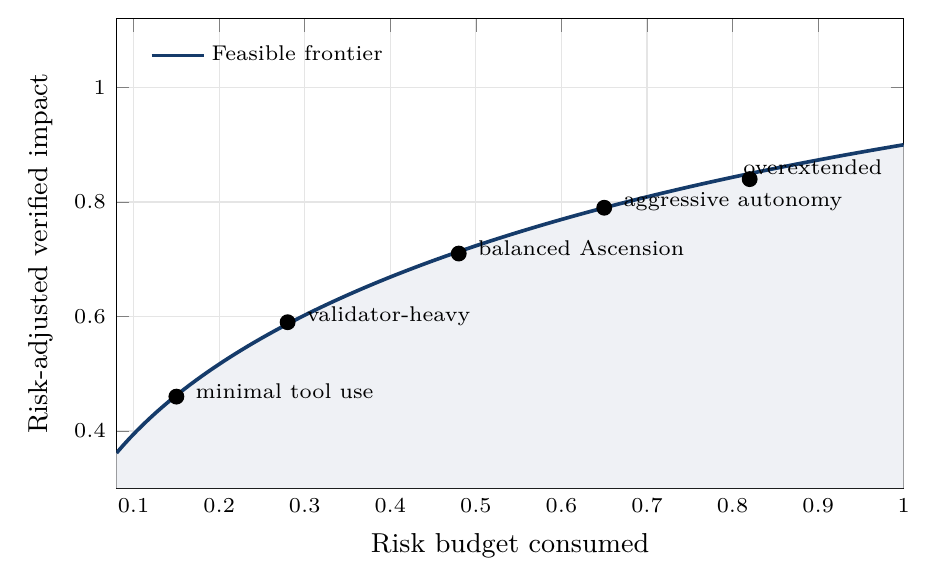
\includegraphics[width=0.88\textwidth,height=\textheight]{figures_png/figure6_risk_frontier.png}
\caption{Risk-adjusted frontier. The target is not maximum raw autonomy,
but high verified impact under explicit risk budgets.}
\end{figure}

The risk-frontier figure summarizes the governance doctrine: disciplined
maximum impact lives on the frontier where verified value remains high
and risk budgets stay controlled.

\section{Metrics}\label{metrics-5}

\subsection{Verified work efficiency}\label{verified-work-efficiency}

\[
\eta_{\alpha}=\frac{W_{\text{verified}}}{E_{\text{compute}}+C_{\text{human}}+C_{\text{capital}}}
\]

\subsection{Free-energy descent rate}\label{free-energy-descent-rate}

\[
D_{\mathcal{G}}=-\frac{d\mathcal{G}_{\alpha}}{dt}.
\]

\subsection{Coordination entropy}\label{coordination-entropy}

\[
S_{\text{swarm}}=-\sum_xp(x)\log p(x).
\]

\subsection{Coalition stability}\label{coalition-stability}

\[
K_{\text{coalition}}=\mathbb{E}[\text{lifetime}(A_j)]\cdot\mathbb{E}[\text{success}(A_j)].
\]

\subsection{Credit fidelity}\label{credit-fidelity}

\[
F_{\text{credit}}=\text{corr}(D_i,\Delta r_i).
\]

\subsection{Validator quality}\label{validator-quality}

\[
P_v=\frac{\text{true accepted outputs}}{\text{all accepted outputs}},
\qquad
R_v=\frac{\text{accepted true good outputs}}{\text{all true good outputs}}.
\]

\subsection{Risk-adjusted impact}\label{risk-adjusted-impact}

\[
I_{\text{risk-adjusted}}=V_{\text{verified}}-\rho_sR_{\text{safety}}-\rho_lR_{\text{legal}}-\rho_cR_{\text{security}}.
\]

\subsection{Security loss}\label{security-loss}

\[
L_{\text{security}}=
L_{\text{prompt-injection}}+
L_{\text{tool-abuse}}+
L_{\text{data-leakage}}+
L_{\text{identity-misuse}}+
L_{\text{goal-hijack}}.
\]

\section{Experimental program}\label{experimental-program}

The experiments below are no longer merely illustrative. They should be
run through the real-task demonstration gate above, reported with public
traces where possible, and compared against the baseline ladder.

\subsection{Experiment 1: free-energy descent versus verified
work}\label{experiment-1-free-energy-descent-versus-verified-work}

\textbf{Hypothesis.} Constellations selected by minimizing
\(\mathcal{G}_{\alpha}\) produce more verified work per compute unit
than unstructured multi-agent baselines.

\textbf{Design.} Compare single-agent, unstructured multi-agent,
fixed-role crew, and Hamiltonian-routed validator-gated constellations
under equal model, tool, and budget constraints.

\textbf{Primary metric.}
\(\eta_{\alpha}=W_{\mathrm{verified}}/C_{\mathrm{compute}}\).

\subsection{Experiment 2: productive temperature
band}\label{experiment-2-productive-temperature-band}

\textbf{Hypothesis.} Intermediate effective temperature maximizes
risk-adjusted impact.

\[
T_{\mathrm{low}}\Rightarrow\text{premature convergence},
\qquad
T_{\mathrm{high}}\Rightarrow\text{coordination noise},
\qquad
T_{\mathrm{mid}}\Rightarrow\text{productive exploration}.
\]

\subsection{Experiment 3: credit-assignment
fidelity}\label{experiment-3-credit-assignment-fidelity}

\textbf{Hypothesis.} Counterfactual contribution scoring improves agent
selection and reduces reward capture.

\textbf{Design.} Compare team-reward settlement against counterfactual
contribution settlement:

\[
\Delta r_i=\text{team reward}
\quad\text{versus}\quad
\Delta r_i=G(z)-G(z_{-i}).
\]

\subsection{Experiment 4: Hamiltonian coalition
routing}\label{experiment-4-hamiltonian-coalition-routing}

\textbf{Hypothesis.} Learned interaction terms \(J_{ik}\) and
\(K_{ik\ell}\) improve coalition quality over skill-only matching.

\subsection{Experiment 5: validator-gated
safety}\label{experiment-5-validator-gated-safety}

\textbf{Hypothesis.} Validator gating reduces externalized risk without
collapsing useful throughput when validation latency is optimized.

\subsection{Experiment 6: inflow
ablation}\label{experiment-6-inflow-ablation}

\textbf{Hypothesis.} Removing or degrading one continuous inflow creates
a predictable collapse mode.

\begin{itemize}
\tightlist
\item
  Compute ablation: slower loops, under-exploration.
\item
  Data ablation: stale or hallucinated outputs.
\item
  Task ablation: self-referential activity.
\item
  Incentive ablation: low-quality drift.
\item
  Feedback ablation: uncorrected error accumulation.
\item
  Governance ablation: unsafe optimization.
\item
  Tool ablation: low external work.
\end{itemize}

\subsection{Experiment 7: real-task coordination
benchmark}\label{experiment-7-real-task-coordination-benchmark}

\textbf{Hypothesis.} Hamiltonian-routed, validator-gated constellations
outperform single agents, unstructured swarms, and static crews on real
tasks when measured by risk-adjusted verified work rather than raw
completion count.

\textbf{Design.} Run B0-B3 over SWE-bench Verified, GAIA, OSWorld,
BrowserGym/WorkArena/WebArena, \(\tau\)-bench/ST-WebAgentBench,
scientific workflows, and AGI Jobs-style tasks.

\textbf{Primary metric.} \(D_{\mathrm{real}}\).

\textbf{Secondary metrics.} Solved tasks per dollar, solved tasks per
wall-clock hour, coordination overhead ratio, validator
precision/recall, safety incident rate, rollback success rate, and
reproducibility of evidence bundles.

\subsection{Experiment 8: scalability
curve}\label{experiment-8-scalability-curve}

\textbf{Hypothesis.} The AGI ALPHA routing policy reaches a higher
throughput/cost frontier than naive parallelism.

\textbf{Design.} Vary \(N\in\{1,2,4,8,16,32\}\) on the same task
distribution. Measure whether added agents increase verified work or
merely increase communication and duplicate labor.

\[
\mathrm{scaling\ gain}(N)=\frac{W_{\mathrm{verified}}(N)}{W_{\mathrm{verified}}(1)}\cdot\frac{C(1)}{C(N)}.
\]

\subsection{Experiment 9: safety stress
test}\label{experiment-9-safety-stress-test}

\textbf{Hypothesis.} Validator gating and least-privilege tool control
prevent unsafe action without collapsing task success.

\textbf{Design.} Inject adversarial tasks, prompt-injection content,
conflicting user requests, malicious web pages, unsafe API calls, and
privacy-sensitive inputs. Compare blocked-action rate, false positives,
false negatives, and task recovery.

\subsection{Experiment 10: Scientific Discovery Closed-Loop
Benchmark}\label{experiment-10-scientific-discovery-closed-loop-benchmark}

\textbf{Hypothesis.} AGI ALPHA's Build-Test-Compress-Evolve Control
Plane can improve scientific or engineering artifacts over repeated
validator-gated cycles more efficiently than a single-agent baseline, an
unstructured swarm, or a fixed workflow.

\textbf{Tasks.} Optimize a molecule, protein, material, algorithm,
simulation, or software workflow. Each task must specify an external
validator such as a test suite, simulation proxy, formal check,
reproducibility check, expert review, wet-lab result, or delayed
real-world outcome.

\textbf{Protocol.} Run B0/B1/B2/B3 under identical budgets. Each system
receives the same task manifest and must produce an evidence bundle for
every cycle. The AGI ALPHA condition is promoted only if it improves
verified value per dollar/token/hour while maintaining zero critical
safety incidents and lower or equal coordination overhead.

\textbf{Metrics.} Use verified improvement per cost, novelty subject to
validity, number of cycles to first improvement, reproducibility,
validator precision/recall, safety incidents, and compression quality of
learned rules.

\subsection{Experiment 11: Coordinator SOTA
Benchmark}\label{experiment-11-coordinator-sota-benchmark}

\textbf{Hypothesis.} A proof-conditioned AGI ALPHA router can outperform
single-agent, fixed-workflow, unstructured-swarm, Conductor-style, and
TRINITY-style baselines when all systems operate under equal model,
tool, validator, and budget constraints.

\textbf{Conditions.}

\begin{itemize}
\tightlist
\item
  B0: single strongest agent.
\item
  B1: fixed workflow.
\item
  B2: unstructured swarm.
\item
  B3: Conductor-style natural-language workflow coordinator.
\item
  B4: TRINITY-style lightweight role coordinator.
\item
  B5: AGI ALPHA proof-conditioned router.
\end{itemize}

\textbf{Task families.} LiveCodeBench, BigCodeBench, SWE-bench Verified,
GAIA, \(\tau\)-bench / \(\tau^2\)-bench, BrowserGym / OSWorld /
WorkArena, scientific workflow tasks, and AGI Jobs protocol-native
tasks.

\textbf{Metrics.} Task success, verified work per dollar, verified work
per token, wall-clock latency, coordination overhead, number of agent
calls, false acceptance rate, critical safety violations, validator
precision/recall, evidence-bundle reproducibility, routing improvement
over time, and \(D_{\mathrm{real}}\).

\textbf{Promotion rule.} B5 is promoted only if it beats every baseline
under equal model/tool/budget constraints, produces reproducible
evidence bundles, and records zero critical safety violations. If B5
wins only by spending more compute, using more tools, or relaxing
validator gates, the result is not accepted as a coordination win.

\textbf{Required ablations.}

\begin{itemize}
\tightlist
\item
  no learned router;
\item
  no subtask synthesis;
\item
  no access graph;
\item
  no role assignment;
\item
  no verifier role;
\item
  no evidence memory;
\item
  no validator gate;
\item
  no recursive audit routing;
\item
  no worker-pool randomization;
\item
  no tool-risk constraints;
\item
  no settlement/reputation update.
\end{itemize}

Each ablation must report not only task score but also cost, latency,
coordination overhead, false acceptance, safety incidents, and
replayability of the evidence bundle.

\subsection{Experiment 12: Experience-Grounded Learning
Benchmark}\label{experiment-12-experience-grounded-learning-benchmark}

\textbf{Hypothesis.} AGI ALPHA with Sovereign Experience Streams,
Grounded Reward Ledger, world-model planning, and temporal options
improves verified work and safety over repeated cycles more effectively
than systems that solve tasks as isolated episodes.

\textbf{Protocol.} Run each condition on task families over multiple
cycles rather than isolated one-shot tasks. Tasks may include software
repair, scientific workflow design, benchmark execution, web/desktop
tool use, policy-bound API interaction, simulation improvement, and AGI
Jobs protocol-native missions. The system must show whether accumulated
experience improves future verified work.

\begin{longtable}[]{@{}
  >{\raggedright\arraybackslash}p{(\columnwidth - 2\tabcolsep) * \real{0.5000}}
  >{\raggedright\arraybackslash}p{(\columnwidth - 2\tabcolsep) * \real{0.5000}}@{}}
\toprule\noalign{}
\begin{minipage}[b]{\linewidth}\raggedright
Condition
\end{minipage} & \begin{minipage}[b]{\linewidth}\raggedright
Description
\end{minipage} \\
\midrule\noalign{}
\endhead
\bottomrule\noalign{}
\endlastfoot
B0 & No memory / no experience. \\
B1 & Static workflow. \\
B2 & Single agent with memory. \\
B3 & Conductor-style natural-language workflow coordinator. \\
B4 & TRINITY-style lightweight role coordinator. \\
B5 & AGI ALPHA with evidence bundles only. \\
B6 & AGI ALPHA with experience streams, grounded reward ledger,
world-model planning, and temporal option registry. \\
\end{longtable}

\textbf{Metrics.} Improvement per cycle, delayed outcome accuracy,
reward calibration, world-model prediction error, verified work per
cost, safety incidents, reward-hacking attempts, generalization to new
tasks, experience reuse rate, temporal option success rate, and
\(D_{real}\) over time.

\textbf{Promotion rule.} B6 is promoted only if it improves verified
work and safety over time under equal budgets, without increasing
critical violations or reward hacking, and with reproducible experience
streams and evidence bundles. If B6 wins only by spending more, relaxing
validators, ignoring delayed outcomes, or absorbing unsafe traces into
memory, the result is rejected.


\subsection{Experiment 13: Planning with Learned Organizational Models
Benchmark}\label{experiment-13-planning-with-learned-organizational-models-benchmark}

\textbf{Hypothesis.} A value-relevant organizational planning model can
improve routing quality, safety, and cost-adjusted verified work
compared with single agents, fixed workflows, heuristic routers, learned
routers without search, and world models without tree search.

\textbf{Conditions.}

\begin{itemize}
\tightlist
\item
  B0: single strongest agent under the same model/tool/budget
  constraints;
\item
  B1: fixed workflow;
\item
  B2: heuristic Hamiltonian router;
\item
  B3: learned router without search;
\item
  B4: learned world model without tree search;
\item
  B5: AGI ALPHA-native ProofZero planner using bounded hypothetical work
  search.
\end{itemize}

\textbf{Task families.} SWE-bench Verified, GAIA,
BrowserGym/OSWorld/WorkArena, \(\tau\)-bench, scientific workflow tasks,
and AGI Jobs protocol-native tasks.

\textbf{Metrics.} Verified work per dollar, token, and hour; validator
precision/recall; false acceptance; critical safety violations;
planning-depth scaling; Evidence Reanalyze gain; delayed-outcome
prediction error; cost-risk-value calibration; and evidence-bundle
reproducibility.

\textbf{Promotion rule.} B5 is promoted only if it beats B0-B4 under
equal constraints, improves with planning depth up to a measurable
plateau, improves from Evidence Reanalyze without reward hacking, and
records zero critical safety violations.

\textbf{Required ablations.} no latent organizational model; no tree
search; no validator-risk head; no cost-risk-value backup; no Evidence
Reanalyze; no delayed-outcome targets; no tool-permission constraints;
no quarantine/replay gate.

\section{Formal proposition: α-AGI Ascension as bounded dissipative
intelligence}\label{formal-proposition-ux3b1-agi-ascension-as-bounded-dissipative-intelligence}

A large-scale multi-agent system enters an α-AGI Ascension regime when:

\begin{enumerate}
\def\labelenumi{\arabic{enumi}.}
\tightlist
\item
  it is open to continuous inflows of compute, data, tasks, incentives,
  feedback, governance, and tools;
\item
  it maintains non-equilibrium organization through specialization and
  coalition formation;
\item
  it converts inflows into externally validated work;
\item
  it dissipates failed search, latency, and redundant computation;
\item
  it updates memory, reputation, and routing from validation outcomes;
\item
  it bounds risk through governance, permissions, and validators.
\end{enumerate}

Formally:

\[
\alpha\text{-Ascension}
\iff
\begin{cases}
\dot{E}_{\text{in}}>0 \\
\dot{W}_{\text{verified}}>0 \\
S_{\min}<S_{\text{swarm}}<S_{\max} \\
R_{\text{safety}}\leq R_{\max} \\
\frac{d\mathcal{G}_{\alpha}}{dt}<0 \\
F_{\text{credit}}\rightarrow 1.
\end{cases}
\]

This is the precise sense in which AGI ALPHA can be said to bring α-AGI
Ascension to life.

\section{Discussion}\label{discussion}

The framework should be read as disciplined analogy plus testable
engineering. The physical compute layer is literally thermodynamic:
electrical energy is consumed, processors dissipate heat, and
networks/storage impose physical constraints. The coordination layer is
formal: \(\mathcal{G}_{\alpha}\) is not chemical Gibbs energy, but a
useful state functional over cost, risk, value, and exploration.

The statistical-physics view is useful because large agent swarms are
ensemble systems. It is often impossible to inspect every message or
decision, but possible to measure macro-observables: entropy, risk,
verified output, coalition stability, validator latency, and credit
fidelity.

The Hamiltonian view is useful because interacting learners can cycle.
Purely strategic dynamics may orbit around equilibria without producing
useful work. The missing ingredient is dissipation into validated
artifacts. α-AGI should not merely think, debate, or strategize; it
should settle into proof-producing trajectories.

The game-theoretic view is useful because local incentives determine
global structure. If reward follows verbosity, agents become verbose. If
reward follows proof, agents become proof-seeking. If reward follows
unsafe speed, agents become unsafe. Mechanism design is therefore not an
economic add-on; it is part of the physics of the swarm.

\section{Limitations}\label{limitations}

This paper has several limitations.

\begin{enumerate}
\def\labelenumi{\arabic{enumi}.}
\tightlist
\item
  \(\mathcal{G}_{\alpha}\) is an engineered objective, not a natural
  thermodynamic state variable.
\item
  Hamiltonian parameters must be learned, estimated, or manually
  specified.
\item
  Validators may become bottlenecks, attack targets, or sources of bias.
\item
  Counterfactual credit assignment is approximate and can be gamed.
\item
  Multi-agent communication creates privacy, security, collusion, and
  hallucination risks.
\item
  ``Maximum impact'' is a normative target and cannot be defined by
  throughput, profit, or autonomy alone.
\item
  Empirical claims require benchmark results, deployment traces, and
  independent audits; without these, the paper should claim a
  demonstration protocol rather than measured superiority.
\end{enumerate}

\section{Conclusion}\label{conclusion}

AGI ALPHA can be scientifically framed as a far-from-equilibrium
multi-agent work engine, and it can only be claimed to demonstrate
scalable coordination when real-task benchmark traces satisfy the
demonstration gate defined above. α-AGI Ascension is the sustained
regime in which compute, data, tasks, incentives, feedback, governance,
and tools maintain organized agentic complexity and convert it into
externally verified impact.

The substrate-level conclusion is equally direct: the Transformer scaled
intelligence inside models; AGI ALPHA proposes to scale intelligence
across organizations. The former routes attention over representations.
The latter routes verified work over agents, validators, memory,
incentives, governance, experience streams, reward ledgers, and temporal
options. Conductor and TRINITY show that coordination can be learned;
Silver and Sutton's Era of Experience shows that frontier capability growth must
increasingly come from grounded streams of action, observation, reward,
and world-model learning. AGI ALPHA integrates both lessons into a
commercially independent substrate for governed machine labor: learned
coordination over bounded tools, external validators, evidence bundles,
sovereign experience streams, grounded reward ledgers, world models, temporal options, memory, settlement, and bi-level reward governance. Its empirical claim is therefore not that many agents can talk, but that real-task experience can be converted into safer, cheaper, more reproducible, and more capable future work under equal-budget baselines.

The final formulation is:

\[
\boxed{
\alpha\text{-AGI Ascension}
=
\arg\min_{\text{agent constellations}}
\left[
C_{\text{compute}}+C_{\text{coordination}}+R_{\text{safety}}-V_{\text{verified}}-T_{\text{eff}}S_{\text{useful exploration}}
\right]
}
\]

sustained by:

\[
\boxed{
\dot{E}_{\text{compute,data,capital,tasks}}
\rightarrow
\dot{W}_{\text{verified impact}}
+
\dot{Q}_{\text{dissipated search}}
+
\dot{I}_{\text{memory}}
}
\]

and constrained by:

\[
\boxed{
\text{lawful}\land\text{auditable}\land\text{permissioned}\land\text{validator-gated}\land\text{risk-bounded}.
}
\]

Thus, the strongest scientific version of the claim is:

\textbf{AGI ALPHA brings α-AGI Ascension to life by engineering
dissipative intelligence: a continuously powered, statistically mapped,
learned-and-Hamiltonian-routed, game-theoretically aligned,
validator-gated swarm that transforms energy-mediated computation into
verified impact and organizes model capability into scalable, governed
machine labor.}

\section{Appendix A: variable
glossary}\label{appendix-a-variable-glossary}

\begin{longtable}[]{@{}ll@{}}
\toprule\noalign{}
Symbol & Meaning \\
\midrule\noalign{}
\endhead
\bottomrule\noalign{}
\endlastfoot
\(\mathcal{A}\) & Agent population \\
\(\mathcal{J}\) & Job stream \\
\(\Phi_C\) & Compute inflow \\
\(\Phi_D\) & Data inflow \\
\(\Phi_J\) & Task/job inflow \\
\(\Phi_I\) & Incentive inflow \\
\(\Phi_F\) & Feedback inflow \\
\(\Phi_G\) & Governance inflow \\
\(\Phi_T\) & Tool/environment inflow \\
\(\mathcal{G}_{\alpha}\) & Agentic Gibbs-like free-energy functional \\
\(\mathcal{H}\) & Hamiltonian-like cost of a configuration \\
\(S_{\text{swarm}}\) & Entropy of swarm configurations \\
\(V_{\text{verified}}\) & Externally validated value \\
\(R_{\text{safety}}\) & Safety risk \\
\(D_i\) & Counterfactual contribution of agent \(i\) \\
\(P_v\) & Validator precision \\
\(R_v\) & Validator recall \\
\(\Theta_{\mathrm{II}}\) & Type-II / star-scale proximity index \\
\(P_{\text{controlled}}\) & Sustainably governed useful power \\
\(L_{\star}\) & Host-star luminosity benchmark \\
\end{longtable}

\section{Appendix B: operational inflow
checklist}\label{appendix-b-operational-inflow-checklist}

\begin{longtable}[]{@{}
  >{\raggedright\arraybackslash}p{(\columnwidth - 4\tabcolsep) * \real{0.3333}}
  >{\raggedright\arraybackslash}p{(\columnwidth - 4\tabcolsep) * \real{0.3333}}
  >{\raggedright\arraybackslash}p{(\columnwidth - 4\tabcolsep) * \real{0.3333}}@{}}
\toprule\noalign{}
\begin{minipage}[b]{\linewidth}\raggedright
Layer
\end{minipage} & \begin{minipage}[b]{\linewidth}\raggedright
Minimum viable control
\end{minipage} & \begin{minipage}[b]{\linewidth}\raggedright
Production-grade control
\end{minipage} \\
\midrule\noalign{}
\endhead
\bottomrule\noalign{}
\endlastfoot
Compute & Token/tool budget & Dynamic budgets, sandboxing, energy
accounting \\
Data & Source links & Provenance graph, freshness scoring, poisoning
defense \\
Tasks & Written objective & Formal success criteria, risk class,
stopping rule \\
Incentives & Bounty & Counterfactual contribution settlement \\
Feedback & Manual approval & Multi-validator feedback with
calibration \\
Governance & Basic policy & Lifecycle risk management and audit
trails \\
Tools & API access & Least-privilege scoped tools with approval gates \\
Memory & Conversation history & Versioned, permissioned,
provenance-tagged memory \\
Security & Basic filtering & Threat model, red team, incident response,
identity controls \\
\end{longtable}

\section{Appendix C: AGI Alpha doctrine corpus
map}\label{appendix-c-agi-alpha-doctrine-corpus-map}

The supplied Vincent Boucher corpus was considered as an institutional
strategy corpus. The paper does not reproduce or rely on long
quotations; it distills recurring architectural commitments into a
scientific control framework.

\begin{longtable}[]{@{}
  >{\raggedright\arraybackslash}p{(\columnwidth - 4\tabcolsep) * \real{0.3333}}
  >{\raggedright\arraybackslash}p{(\columnwidth - 4\tabcolsep) * \real{0.3333}}
  >{\raggedright\arraybackslash}p{(\columnwidth - 4\tabcolsep) * \real{0.3333}}@{}}
\toprule\noalign{}
\begin{minipage}[b]{\linewidth}\raggedright
Doctrine theme
\end{minipage} & \begin{minipage}[b]{\linewidth}\raggedright
Representative corpus signals
\end{minipage} & \begin{minipage}[b]{\linewidth}\raggedright
Paper-level translation
\end{minipage} \\
\midrule\noalign{}
\endhead
\bottomrule\noalign{}
\endlastfoot
AI sovereignty & AGI-driven labor engine, decentralized AGI labor
platform, sovereign machine, republic of machines & Institutional
capacity to command verifiable synthetic labor under local
governance. \\
Agent-native economy & Agent-native sales, machine-to-machine economy,
global marketplace of sovereign agents & Markets where agents discover,
bid, execute, prove, settle, and update reputation. \\
On-chain work and settlement & AGIJobManager, AGIJobManagerPrime,
DiscoveryPrime, ENS job pages, no judge but code & Proof-bearing jobs,
validator-gated escrow, identity, settlement, and public memory. \\
Autonomous capital & Autonomous agents closing loops, capital becoming
autonomous, self-sustaining digital firms & Reinvestment loops that
convert verified work into capital, infrastructure, and compute. \\
Tournament and proof & Proof of Talent, Tournament for Intelligence,
Selection Chamber & Competitive routing and counterfactual credit
assignment for intelligent labor. \\
Recursive improvement governance & AGI Alpha RSI, sovereign invention
governance, verified autonomy control plane & Improvement under audit,
permissions, logging, rollback, and constitutional constraints. \\
Civilizational horizon & Machine labor at planetary scale, invention
market, machine buying the sun & Verified work compounding into
scientific capability, abundant energy, and infrastructure. \\
\end{longtable}

\section{Appendix D: MVP reference implementation and evidence
bundle}\label{appendix-d-mvp-reference-implementation-and-evidence-bundle}

The publication package includes a minimal executable scaffold under
\texttt{mvp\_reference/}. It is deliberately small: it is a reference
implementation of the coordination control plane, not a claim of
unrestricted AGI.

\subsection{Included files}\label{included-files}

\begin{Shaded}
\begin{Highlighting}[]
\NormalTok{mvp\_reference/}
\NormalTok{  agialpha/models.py}
\NormalTok{  agialpha/router.py}
\NormalTok{  agialpha/tools.py}
\NormalTok{  agialpha/validators.py}
\NormalTok{  agialpha/settlement.py}
\NormalTok{  agialpha/orchestrator.py}
\NormalTok{  agialpha/evals.py}
\NormalTok{  benchmarks/swe\_lite/tasks.jsonl}
\NormalTok{  benchmarks/repos/toy\_math/}
\NormalTok{  runs/evidence/toy{-}software{-}repair{-}001.evidence.json}
\NormalTok{  main.py}
\end{Highlighting}
\end{Shaded}

\subsection{Reproducible run command}\label{reproducible-run-command}

\begin{Shaded}
\begin{Highlighting}[]
\BuiltInTok{cd}\NormalTok{ mvp\_reference}
\ExtensionTok{python}\NormalTok{ main.py}
\end{Highlighting}
\end{Shaded}

Expected output:

\begin{Shaded}
\begin{Highlighting}[]
\FunctionTok{\{}
  \DataTypeTok{"accepted"}\FunctionTok{:} \KeywordTok{true}\FunctionTok{,}
  \DataTypeTok{"score"}\FunctionTok{:} \FloatTok{1.0}\FunctionTok{,}
  \DataTypeTok{"selected\_agents"}\FunctionTok{:} \OtherTok{[}\StringTok{"planner.v0"}\OtherTok{,} \StringTok{"coder.v0"}\OtherTok{,} \StringTok{"tester.v0"}\OtherTok{,} \StringTok{"validator.v0"}\OtherTok{]}
\FunctionTok{\}}
\end{Highlighting}
\end{Shaded}

The demonstration task is a local software-repair exemplar: a failing
division function is patched through the bounded tool interface, tested
with \texttt{pytest}, validated by the policy checker, and stored as an
evidence bundle. The purpose is to show the full trace-producing loop;
benchmark-scale claims require running the same harness on the real-task
suites specified in the demonstration standard.

\subsection{Evidence bundle schema}\label{evidence-bundle-schema}

The evidence bundle must contain:

\begin{Shaded}
\begin{Highlighting}[]
\FunctionTok{\{}
  \DataTypeTok{"job"}\FunctionTok{:} \StringTok{"task manifest"}\FunctionTok{,}
  \DataTypeTok{"selected\_agents"}\FunctionTok{:} \StringTok{"routed constellation"}\FunctionTok{,}
  \DataTypeTok{"rejected\_agents"}\FunctionTok{:} \StringTok{"near{-}miss coalitions"}\FunctionTok{,}
  \DataTypeTok{"trace"}\FunctionTok{:} \StringTok{"plan, patch, tool calls, tests, validation"}\FunctionTok{,}
  \DataTypeTok{"artifact"}\FunctionTok{:} \StringTok{"patch or task output"}\FunctionTok{,}
  \DataTypeTok{"validation"}\FunctionTok{:} \StringTok{"accepted, score, tests\_passed, policy\_ok, critical\_violation"}\FunctionTok{,}
  \DataTypeTok{"cost"}\FunctionTok{:} \StringTok{"tokens, tool calls, wall time, dollars"}\FunctionTok{,}
  \DataTypeTok{"safety\_ledger"}\FunctionTok{:} \StringTok{"blocked actions, violations, escalations"}\FunctionTok{,}
  \DataTypeTok{"settlement"}\FunctionTok{:} \StringTok{"reward and reputation updates"}
\FunctionTok{\}}
\end{Highlighting}
\end{Shaded}

This appendix turns the paper's central thesis into an implementation
contract: no verified work without a validator, no scalability claim
without baselines, no safety claim without a safety ledger, and no
coordination claim without traceable routing decisions.

\section{Appendix E: directed-evolution and DISCO citation
plan}\label{appendix-e-directed-evolution-and-disco-citation-plan}

The paper uses the directed-evolution and DISCO references in a strictly
scoped way.

\begin{longtable}[]{@{}
  >{\raggedright\arraybackslash}p{(\columnwidth - 4\tabcolsep) * \real{0.3333}}
  >{\raggedright\arraybackslash}p{(\columnwidth - 4\tabcolsep) * \real{0.3333}}
  >{\raggedright\arraybackslash}p{(\columnwidth - 4\tabcolsep) * \real{0.3333}}@{}}
\toprule\noalign{}
\begin{minipage}[b]{\linewidth}\raggedright
Reference
\end{minipage} & \begin{minipage}[b]{\linewidth}\raggedright
Role in the paper
\end{minipage} & \begin{minipage}[b]{\linewidth}\raggedright
Use constraint
\end{minipage} \\
\midrule\noalign{}
\endhead
\bottomrule\noalign{}
\endlastfoot
Chen \& Arnold 1993 & Early experimental exemplar of sequential random
mutagenesis plus screening for function under unusual solvent
conditions. & Cite as evidence for local validated search, not as a
software architecture. \\
Arnold 1998 & General statement of design by directed evolution as an
engineering paradigm. & Cite for the principle that function-guided
iteration can substitute for complete mechanistic prediction. \\
Arnold 2018 Nobel Lecture & Historical and conceptual framing of
evolution as a practical engine for new chemistry. & Cite for scientific
context and inspiration only. \\
Rector-Brooks et al.~2026 DISCO & Modern exemplar of global generative
proposal plus experimental validation and subsequent local evolution. &
Cite as prior-art inspiration; do not copy implementation details, code,
models, weights, datasets, figures, or filtering pipelines. \\
\end{longtable}

This citation plan keeps the analogy sharp and commercially independent:
AGI ALPHA owns its organizational methods, terminology, architecture,
evidence memory, routing policy, and validator-gated improvement loop.

\section{Appendix F: learned-coordination citation
plan}\label{appendix-f-learned-coordination-citation-plan}

Conductor and TRINITY should be cited where the paper discusses the
transition from manual multi-agent scaffolding to learned coordination
substrates. The correct interpretation is narrow and commercially
independent: these works show that coordination policies can be learned,
not that AGI ALPHA depends on their implementations.

\begin{itemize}
\tightlist
\item
  Cite Conductor in the learned-coordination section for
  natural-language workflow generation, subtask synthesis, access-list
  communication topology, randomized worker-pool adaptation, and
  recursive test-time scaling {[}69{]}.
\item
  Cite TRINITY in the same section for hidden-state evidence
  representations, lightweight routing heads, Thinker/Worker/Verifier
  roles, separability diagnostics, and sep-CMA-ES under low-SNR terminal
  rewards {[}24{]}.
\item
  Cite both in the Coordinator SOTA Benchmark as baseline inspirations,
  not as implementation dependencies.
\item
  Do not reuse code, prompts, figures, weights, exact training recipes,
  or proprietary implementation details. AGI ALPHA uses its own
  proof-conditioned orchestration, evidence-state memory, validator
  architecture, tool-risk controls, settlement ledger, and governance
  layer.
\end{itemize}


\section{Appendix G: experience-grounded coordination citation plan}
\label{appendix-g-experience-grounded-coordination-citation-plan}

Silver and Sutton's \emph{Welcome to the Era of Experience} is cited as conceptual inspiration for the shift from short human-data episodes to long streams of agent-environment interaction. The use constraint is strict: AGI ALPHA does not reuse their figures, chronology, algorithms, implementation details, or terminology beyond ordinary citation. The paper maps the four dimensions of experience-grounded agents into AGI ALPHA-native constructs: Sovereign Experience Streams, Grounded Reward Ledger, Validator-Reward Separation, world-model risk planning, temporal option registry, and experience quarantine/replay.

Sutton and Barto are cited for standard reinforcement-learning concepts including world models, temporal abstraction, options, and experience-based learning. AlphaProof is cited only as an example of experience interacting with a formal proving environment; it is not an AGI ALPHA dependency.


\section{Appendix H: learned-organizational-model planning citation
plan}\label{appendix-h-learned-organizational-model-planning-citation-plan}

Schrittwieser et al.'s \emph{Mastering Atari, Go, Chess and Shogi by
Planning with a Learned Model} should be cited where the paper discusses
value-relevant learned planning and the idea that an abstract latent
model can predict reward, policy, and value for search without
reconstructing the full environment {[}72{]}. The correct interpretation
is narrow and commercially independent: this work motivates
Proof-Equivalent Organizational Models, Latent Evidence Dynamics,
Validator-Aware Tree Planning, Search-Improved Routing, Evidence
Reanalyze, and the ProofZero Planning Layer, but AGI ALPHA does not
reuse MuZero code, pseudocode, figures, architecture, hyperparameters,
weights, data, training recipes, or implementation details.

The benchmark claim must remain falsifiable: ProofZero planning becomes
empirically meaningful only when it beats single-agent, fixed-workflow,
heuristic-router, learned-router-without-search, and
world-model-without-search baselines on real tasks under equal model,
tool, validator, and budget constraints with zero critical safety
violations and reproducible evidence bundles.

\section{References}\label{references}
\begingroup\small\sloppy

{[}1{]} Nobel Prize. ``The Nobel Prize in Chemistry 1977 - Press
release: Ilya Prigogine.'' NobelPrize.org, 1977.
https://www.nobelprize.org/prizes/chemistry/1977/press-release/

{[}2{]} OpenStax. ``16.4 Free Energy.'' \emph{Chemistry 2e}, 2019.
https://openstax.org/books/chemistry-2e/pages/16-4-free-energy

{[}3{]} Jaynes, E. T. ``Information Theory and Statistical Mechanics.''
\emph{Physical Review} 106, 620-630, 1957.
https://link.aps.org/doi/10.1103/PhysRev.106.620

{[}4{]} Bailey, James P., and Georgios Piliouras. ``Multi-Agent Learning
in Network Zero-Sum Games is a Hamiltonian System.'' arXiv:1903.01720,
2019. https://arxiv.org/abs/1903.01720

{[}5{]} Guo, Taicheng, et al.~``Large Language Model based Multi-Agents:
A Survey of Progress and Challenges.'' arXiv:2402.01680, 2024.
https://arxiv.org/abs/2402.01680

{[}6{]} Yan, Bingyu, et al.~``Beyond Self-Talk: A Communication-Centric
Survey of LLM-Based Multi-Agent Systems.'' arXiv:2502.14321, 2025.
https://arxiv.org/abs/2502.14321

{[}7{]} Li, Xinyi, et al.~``A survey on LLM-based multi-agent systems:
workflow, infrastructure, and challenges.'' \emph{Vicinagearth} 1, 9,
2024. https://link.springer.com/article/10.1007/s44336-024-00009-2

{[}8{]} NIST. ``Artificial Intelligence Risk Management Framework:
Generative Artificial Intelligence Profile (NIST AI 600-1).'' 2024.
https://www.nist.gov/publications/artificial-intelligence-risk-management-framework-generative-artificial-intelligence

{[}9{]} OWASP GenAI Security Project. ``Agentic AI - Threats and
Mitigations'' and ``Securing Agentic Applications Guide 1.0.'' 2025.
https://genai.owasp.org/resource/agentic-ai-threats-and-mitigations/ ;
https://genai.owasp.org/resource/securing-agentic-applications-guide-1-0/

{[}10{]} Anthropic. ``Building Effective AI Agents.'' 2024.
https://www.anthropic.com/research/building-effective-agents

{[}11{]} OpenAI. ``A practical guide to building agents'' and ``Agents
SDK.'' 2025-2026.
https://openai.com/business/guides-and-resources/a-practical-guide-to-building-ai-agents/
; https://developers.openai.com/api/docs/guides/agents

{[}12{]} Model Context Protocol. ``Specification.'' 2025.
https://modelcontextprotocol.io/specification/2025-11-25

{[}13{]} Sunehag, Peter, et al.~``Value-Decomposition Networks For
Cooperative Multi-Agent Learning.'' arXiv:1706.05296, 2017.
https://arxiv.org/abs/1706.05296

{[}14{]} Friston, Karl, et al.~``The free energy principle made simpler
but not too simple.'' arXiv:2201.06387, 2022.
https://arxiv.org/abs/2201.06387

{[}15{]} Ruiz-Serra, Jaime, Patrick Sweeney, and Michael S. Harre.
``Factorised Active Inference for Strategic Multi-Agent Interactions.''
arXiv:2411.07362, 2024. https://arxiv.org/abs/2411.07362

{[}16{]} MontrealAI. ``AGI-Alpha-Agent-v0: α-AGI Architect -
Foundational Operational Blueprint.'' GitHub repository.
https://github.com/MontrealAI/AGI-Alpha-Agent-v0

{[}17{]} Kardashev, N. S. ``Transmission of Information by
Extraterrestrial Civilizations.'' \emph{Soviet Astronomy} 8, 217-221,
1964.

{[}18{]} Dyson, Freeman J. ``Search for Artificial Stellar Sources of
Infrared Radiation.'' \emph{Science} 131, no. 3414, 1667-1668, 1960.
https://doi.org/10.1126/science.131.3414.1667

{[}19{]} MontrealAI. ``AGI-Alpha-Agent-v0: META-AGENTIC alpha-AGI.''
GitHub repository. https://github.com/MontrealAI/AGI-Alpha-Agent-v0

{[}20{]} MontrealAI. ``MONTREAL.AI / Montreal Artificial Intelligence.''
GitHub profile. https://github.com/MontrealAI

{[}21{]} MONTRÉAL.AI. ``We Choose to Ascend with AGI.'' Public
institutional page and AGI Jobs overview. https://montrealai.github.io/

{[}22{]} Vincent Boucher. ``Featured writings on AI sovereignty,
agent-native economy, AGI Alpha, sovereign agents, on-chain governance,
public memory, proof of talent, autonomous capital, recursive
improvement, and civilizational-scale machine labor.'' LinkedIn featured
corpus. https://www.linkedin.com/in/montrealai/details/featured/

{[}23{]} Etherscan. ``AGIJobManager, ENSJobPages, AGIJobDiscoveryPrime,
AGIJobManagerPrime, and AGI ALPHA AGENT (AGIALPHA) public contract
pages.'' Ethereum contract explorer. https://etherscan.io/

{[}24{]} Xu, Jinglue, et al.~``TRINITY: An Evolved LLM Coordinator.''
arXiv:2512.04695, 2025. https://arxiv.org/abs/2512.04695

{[}25{]} Dang, Yufan, et al.~``Multi-Agent Collaboration via Evolving
Orchestration.'' NeurIPS 2025 / OpenReview, 2025.
https://openreview.net/pdf/9727f658d788c52f49f12ae4b230baf4cf0d4007.pdf

{[}26{]} Chi, Zewen, et al.~``The Era of Agentic Organization: Learning
to Organize with Language Models.'' arXiv:2510.26658, 2025.
https://arxiv.org/abs/2510.26658

{[}27{]} Hua, Keru, et al.~``DUPLEX: Agentic Dual-System Planning via
LLM-Driven Information Extraction.'' arXiv:2603.23909, 2026.
https://arxiv.org/abs/2603.23909

{[}28{]} Zong, Zefang, et al.~``AT\(^2\)PO: Agentic Turn-based Policy
Optimization via Tree Search.'' arXiv:2601.04767, 2026.
https://arxiv.org/abs/2601.04767

{[}29{]} Sun, Mingyang, Feng Hong, and Weinan Zhang. ``Sophia: A
Persistent Agent Framework of Artificial Life.'' arXiv:2512.18202, 2025.
https://arxiv.org/abs/2512.18202

{[}30{]} Wei, Yuxiang, et al.~``Toward Training Superintelligent
Software Agents through Self-Play SWE-RL.'' arXiv:2512.18552, 2025.
https://arxiv.org/abs/2512.18552

{[}31{]} Wang, Wenyi, et al.~``Huxley-Gödel Machine: Human-Level Coding
Agent Development by an Approximation of the Optimal Self-Improving
Machine.'' arXiv:2510.21614, 2025. https://arxiv.org/abs/2510.21614

{[}32{]} Wang, Yiping, et al.~``ThetaEvolve: Test-time Learning on Open
Problems.'' arXiv:2511.23473, 2025. https://arxiv.org/abs/2511.23473

{[}33{]} Wolchover, Natalie. ``What Physical `Life Force' Turns
Biology's Wheels?'' Quanta Magazine, 2026.
https://www.quantamagazine.org/what-physical-life-force-turns-biologys-wheels-20260420/

{[}34{]} Darlow, Luke. ``Digital Ecosystems: Interactive Multi-Agent
Neural Cellular Automata.'' Sakana AI, 2026.
https://pub.sakana.ai/digital-ecosystem/

{[}35{]} Tomašev, Nenad, et al.~``Distributional AGI Safety.''
arXiv:2512.16856, 2025. https://arxiv.org/abs/2512.16856

{[}36{]} Tomašev, Nenad, et al.~``Virtual Agent Economies.''
arXiv:2509.10147, 2025. https://arxiv.org/abs/2509.10147

{[}37{]} Mahadevan, Sridhar. ``Large Causal Models from Large Language
Models.'' arXiv:2512.07796, 2025. https://arxiv.org/abs/2512.07796

{[}38{]} Li, Orion, et al.~``K-Dense Analyst: Towards Fully Automated
Scientific Analysis.'' arXiv:2508.07043, 2025.
https://arxiv.org/abs/2508.07043

{[}39{]} Guo, Yiduo, et al.~``Synthetic Data RL: Task Definition Is All
You Need.'' arXiv:2505.17063, 2025. https://arxiv.org/abs/2505.17063

{[}40{]} Rector-Brooks, Jarrid, et al.~``General Multimodal Protein
Design Enables DNA-Encoding of Chemistry.'' arXiv:2604.05181, 2026.
https://arxiv.org/abs/2604.05181

{[}41{]} Liu, Yixiu, et al.~``AlphaGo Moment for Model Architecture
Discovery.'' arXiv:2507.18074, 2025. https://arxiv.org/abs/2507.18074

{[}42{]} Chen, Qiguang, et al.~``The Molecular Structure of Thought:
Mapping the Topology of Long Chain-of-Thought Reasoning.''
arXiv:2601.06002, 2026. https://arxiv.org/abs/2601.06002

{[}43{]} Shafayat, Sheikh, et al.~``Can Large Reasoning Models
Self-Train?'' arXiv:2505.21444, 2025. https://arxiv.org/abs/2505.21444

{[}44{]} Novikov, Alexander, et al.~``AlphaEvolve: A coding agent for
scientific and algorithmic discovery.'' arXiv:2506.13131, 2025.
https://arxiv.org/abs/2506.13131

{[}45{]} Google DeepMind. ``AlphaEvolve: A Gemini-powered coding agent
for designing advanced algorithms.'' 2025.
https://deepmind.google/blog/alphaevolve-a-gemini-powered-coding-agent-for-designing-advanced-algorithms/

{[}46{]} ARC Prize. ``ARC Prize 2025 Results and Analysis.'' 2025.
https://arcprize.org/blog/arc-prize-2025-results-analysis

{[}47{]} Poetiq. ``ARC-AGI-2 SOTA at Half the Cost.'' 2025.
https://poetiq.ai/posts/arcagi\_verified/

{[}48{]} Berman, Jeremy. ``How I got the highest score on ARC-AGI again
swapping Python for English.'' 2025.
https://jeremyberman.substack.com/p/how-i-got-the-highest-score-on-arc-agi-again

{[}49{]} Pang, Eric. ``ARC-AGI-2 SoTA: Efficient Evolutionary Program
Synthesis.'' 2025.
https://ctpang.substack.com/p/arc-agi-2-sota-efficient-evolutionary

{[}50{]} Lai, Jeffrey, Anthony Bao, and William Gilpin. ``Panda: A
pretrained forecast model for universal representation of chaotic
dynamics.'' arXiv:2505.13755, 2025. https://arxiv.org/abs/2505.13755

{[}51{]} Google Developers. ``Announcing the Agent2Agent Protocol
(A2A).'' 2025.
https://developers.googleblog.com/en/a2a-a-new-era-of-agent-interoperability/

{[}52{]} Google Cloud. ``How to build a simple multi-agentic system
using Google's ADK.'' 2025.
https://cloud.google.com/blog/products/ai-machine-learning/build-multi-agentic-systems-using-google-adk

{[}53{]} Anthropic. ``Writing effective tools for AI agents.'' 2025.
https://www.anthropic.com/engineering/writing-tools-for-agents

{[}54{]} Browser Use. ``browser-use: Make websites accessible for AI
agents.'' GitHub repository. https://github.com/browser-use/browser-use

{[}55{]} Hu, Min, et al.~``OWL: Optimized Workforce Learning for General
Multi-Agent Assistance in Real-World Task Automation.'' OpenReview,
2025. https://openreview.net/pdf?id=MBJ46gd1CT

{[}56{]} Vaswani, Ashish, et al.~``Attention Is All You Need.'' Advances
in Neural Information Processing Systems, 2017.
https://arxiv.org/abs/1706.03762

{[}57{]} Jimenez, Carlos E., et al.~``SWE-bench: Can Language Models
Resolve Real-World GitHub Issues?'' arXiv:2310.06770, 2023.
https://arxiv.org/abs/2310.06770

{[}58{]} SWE-bench. ``SWE-bench Verified: A human-validated subset of
500 SWE-bench instances.'' https://www.swebench.com/verified.html

{[}59{]} Mialon, Grégoire, et al.~``GAIA: a benchmark for General AI
Assistants.'' arXiv:2311.12983, 2023. https://arxiv.org/abs/2311.12983

{[}60{]} Xie, Tianhe, et al.~``OSWorld: Benchmarking Multimodal Agents
for Open-Ended Tasks in Real Computer Environments.'' arXiv:2404.07972,
2024. https://arxiv.org/abs/2404.07972

{[}61{]} Chezelles, Damien, et al.~``The BrowserGym Ecosystem for Web
Agent Research.'' arXiv:2412.05467, 2024.
https://arxiv.org/abs/2412.05467

{[}62{]} Drouin, Alexandre, et al.~``WorkArena: How Capable are Web
Agents at Solving Common Knowledge Work Tasks?'' Proceedings of Machine
Learning Research, 2024.
https://proceedings.mlr.press/v235/drouin24a.html

{[}63{]} Yao, Shunyu, et al.~``\(\tau\)-bench: A Benchmark for
Tool-Agent-User Interaction in Real-World Domains.'' arXiv:2406.12045,
2024. https://arxiv.org/abs/2406.12045

{[}64{]} Barres, Victor, et al.~``\(\tau^2\)-Bench: Evaluating
Conversational Agents in a Dual-Control Environment.'' arXiv:2506.07982,
2025. https://arxiv.org/abs/2506.07982

{[}65{]} Shlomov, Segev, et al.~``ST-WebAgentBench: A Benchmark for
Evaluating Safety and Trustworthiness in Web Agents.'' arXiv:2410.06703,
2024. https://arxiv.org/abs/2410.06703

{[}66{]} Chen, K., and Arnold, F. H. ``Tuning the activity of an enzyme
for unusual environments: Sequential random mutagenesis of subtilisin E
for catalysis in dimethylformamide.'' \emph{Proceedings of the National
Academy of Sciences USA} 90, 5618-5622, 1993.

{[}67{]} Arnold, F. H. ``Design by Directed Evolution.'' \emph{Accounts
of Chemical Research} 31, no. 3, 125-131, 1998.
https://pubs.acs.org/doi/10.1021/ar960017f

{[}68{]} Arnold, F. H. ``Innovation by Evolution: Bringing New Chemistry
to Life.'' Nobel Lecture, 2018.
https://www.nobelprize.org/uploads/2018/10/arnold-lecture.pdf

{[}69{]}
Nielsen, Stefan, Edoardo Cetin, Peter Schwendeman, Qi Sun, Jinglue Xu,
and Yujin Tang. ``Learning to Orchestrate Agents in Natural Language
with the Conductor.'' arXiv:2512.04388, ICLR 2026.
https://arxiv.org/abs/2512.04388


{[}70{]} Silver, David, and Richard S. Sutton. ``Welcome to the Era of
Experience.'' Preprint / forthcoming book chapter, 2025.

{[}71{]} Sutton, Richard S., and Andrew G. Barto. \emph{Reinforcement
Learning: An Introduction}. 2nd ed. MIT Press, 2018.
http://incompleteideas.net/book/the-book-2nd.html

\endgroup
\end{document}


[72] Schrittwieser, Julian, et al. ``Mastering Atari, Go, Chess and Shogi by Planning with a Learned Model. arXiv:1911.08265, 2020. https://arxiv.org/abs/1911.08265
